\chapter{集合论}

\section{收集化关系}

\subsection{集合论}

集合论是一种包含关系符号的理论 \(=,\) \(\in\) 以及实质性的符号 \(\supset\) (所有这些符号的权均为2)；除了第一章中给出的模式S1至S7外，它还包含将在第6节中引入的模式S8，以及显式公理A1（第3节）、A2（第5节）、A3（ \(\S\) 2，第1号），A4（ \(\S\) 5，第1期），以及A5（第三章， \(\S\) 6，第1期），这些显式公理不包含任何字母；换言之，集合论是一个没有常量的理论。

由于集合论是一种平等理论，第一章的结果适用。

从现在起，除非另有明确说明，我们总是在比集合论更强的理论（第一章，§2，第4节）中进行论证；如果未提及该理论，则假定隐含集合论。在许多情况下，这一假设显然是多余的，读者应不难确定所陈述的结果在何种弱于集合论的理论中成立。

如果T和U是项，则这个汇编 \(\in TU\) 是一个关系（称为属于关系），在实际中我们通常以下列方式之一书写： \(\widetilde{T} \in U\) , \((\widetilde{T}) \in (U)\) “T 属于 U”，“T 是 U 的一个元素”。关系“不 \((\widetilde{T} \in U)\) '' 写作 \(T \notin U\) .

从“朴素”的观点来看，许多数学实体可以被视为对象的集合或“集”。我们不寻求将这一概念形式化，在后续内容的形式主义解释中，“集”一词应严格视为“项”的同义词。特别是，诸如“设X为一个集”这样的短语，原则上完全是多余的，因为每个字母都是一个项。引入这些短语仅是为了帮助对文本的直观理解。

\subsection{包含关系}

定义1. 用以下记号表示的关系 \((\forall z)((z \in x) \Longrightarrow (z \in y))\) ，其中只出现字母 \(x\) 和 \(y\) ，按以下方式之一书写： \(x \subset y\) , \(y \supset x\) , `` \(x\) 包含于 \(y\) '', `` \(y\) 包含 \(x\) '', `` \(x\) 是 \(y\) 的子集''。关系“不 \((x \subset y)\) '' 写作 \(x \not\subset y\) 或 \(y \not\supset x\) .

按照第一章第1节第1号中提到的约定，这个定义蕴含以下元数学约定。设T和U为汇编；若我们在汇编 \(x \subset y\) 中将T替换为x、将U替换为y，我们得到一个汇编，记为 \(T \subset U\) ；如果我们用 x，y 表示与 x，y 不同且彼此不同的字母，并且它们既不出现在 T 中也不出现在 U 中，则汇编 \(T \subset U\) 恒同于 \((T|x)(U|y)(x|x)(y|y)(x \subset y,)\) ，因此由 CS8、CS9（第一章，§4，第 1 号）以及 CS5（第一章，§1，第 2 号），它恒同于 \((\forall z)((z \in T) \Longrightarrow (z \in U))\) ，前提是 z 是一个既不出现在 T 中也不出现在 U 中的字母。

从现在起，每当我们陈述一个数学定义时，我们将不再提及它所蕴含的元数学约定。

CS12。设 \(\pmb{T},\pmb{U},\pmb{V}\) 为组装，并设 \(\pmb{x}\) 是一个字母。则汇编 \((\pmb{V}|\pmb{x})(\pmb{T}\subset \pmb{U})\) 恒同于 \((\pmb{V}|\pmb{x})\pmb{T}\subset (\pmb{V}|\pmb{x})\pmb{U}\) .

这直接从 CS9（第一章，§4，第 1 号）和 CS5（第一章，§1，第 2 号）得出。

CF13。如果 \(\pmb{T}\) 并且 \(\pmb{U}\) 是项， \(\pmb{T} \subset \pmb{U}\) 是一个关系。

这直接从CF8（第一章，§1，第4节）得出。

¶ 每个形如 \(T \subset U\) （其中 T 和 U 是项）的关系称为包含关系。

从现在起，我们不再明确写出替换准则以及应在定义之后给出的构成准则。但应注意，这些准则在证明中常常会被隐式使用。

为了证明该关系 \(x \subset y\) 在一个理论中 \(\mathfrak{G}\) ，根据C27（第一章，§4，第1号），只需证明 \(z \in y\) 在通过附加 \(z \in x\) 对于公理 \(\mathfrak{G}\) ，其中 \(z\) 是一个与 \(x, y\) 以及理论的常数。在实践中我们说“令 \(z\) 为 \(x\) ''，并且我们试图证明 \(z \in y\) .

命题1。 \(x \subset x\) .

显然。

命题2。 \((x\subset y\) 并且 \(y\subset z)\Longrightarrow (x\subset z).\)

添加假设 \(x \subset y, y \subset z\) ，以及 \(u \in x\) 。则关系

\[
(u \in x) \Longrightarrow (u \in y), \quad (u \in y) \Longrightarrow (u \in z),
\]

为真，因此该关系 \(u \in z\) 为真。

\subsection{外延公理}

外延公理如下：

A1.

\[
(\forall x) (\forall y) ((x \subset y \text {   且   } y \subset x) \Longrightarrow (x = y)).
\]

直观上，这条公理表达了两个具有相同元素的集合是相等的这一事实。

为了证明 x = y，因此只需证明 \(z \in y\) 在通过附加该假设所得的理论中 \(z \in x\) ，以及 \(z \in x\) 在通过附加该假设所得的理论中 \(z \in y\) ，其中 z 是一个不同于 x、y 及常量的字母。

C48. 设 R 是一个关系，x 是一个字母，y 是一个不同于 x 且不出现在 R 中的字母。则关系 \((\forall x)((x \in y) \Longleftrightarrow R)\) 在 y 上是单值的。

让 \(\pmb{z}\) 是一个与 \(\pmb{x}\) 的字母，它不出现在 \(\pmb{R}\) 。添加假设

\[
(\forall x) ((x \in y) \Longleftrightarrow R), (\forall x) ((x \in z) \Longleftrightarrow R).
\]

于是我们依次有定理

\[
\begin{array}{c} (\forall x) (((x \in y) \Longleftrightarrow R) \quad \text { 且 } \quad ((x \in z) \Longleftrightarrow R)), \\ (\forall x) ((x \in y) \Longleftrightarrow (x \in z)), \\ y \subset z, \qquad z \subset y. \end{array}
\]

由 A1 我们得到 y = z。这证明了 C48。

\subsection{集合化关系}

设 R 是一个关系，x 是一个字母。如果 y 和 \(y'\) 表示不同于 x 且不出现在 R 中的字母，则关系

\[
(\exists y) (\forall x) ((x \in y) \leftrightarrow R), (\exists y ^ {\prime}) (\forall x) ((x \in y ^ {\prime}) \leftrightarrow R)
\]

由 CS8（第一章，§4，第1号），二者相同。如此定义的关系（其中不含 x）记为 Coll \(_{x}\) R.

如果 \(\operatorname{Coll}_{\mathbf{x}} R\) 是理论 \(\mathcal{G}\) 中的一个定理，就称 \(R\) 关于 \(\mathbf{x}\) 在 \(\mathcal{G}\) 中是集合化的。在这种情况下，可以引入一个辅助常量 \(\mathbf{a}\) ，它异于 \(\mathbf{x}\) 和 \(\mathcal{G}\) 的各常量，且不出现在 \(\mathbf{R}\) 中，同时引入公理 \((\forall \mathbf{x}) ((\mathbf{x} \in \mathbf{a}) \Longleftrightarrow \mathbf{R})\) ；等价地，如果 \(\mathbf{x}\) 不是 \(\mathcal{G}\) 的常量，则引入 \((\mathbf{x} \in \mathbf{a}) \Longleftrightarrow \mathbf{R}\) .

直观地说，说R在x中收集，就是说存在一个集合a，使得具有性质R的对象x恰好是a的元素。

\minorheading{示例}

\begin{enumerate}
\def\labelenumi{(\arabic{enumi})}
\item
  关系 \(x \in y\) 显然关于 \(x\) 是集合化的.
\item
  关系 \(x \notin x\) 关于 \(x\) 不是集合化的；换言之，（非 \(\operatorname{Coll}_x(x \notin x)\) ) 是一个定理。用反证法证明：假设 \(x \notin x\) 是集合化的。设 \(a\) 为一个辅助常量，它异于 \(x\) 和该理论的各常量，并取引入公理
\end{enumerate}

\[
(\forall x) ((x \notin x) \iff (x \in a)).
\]

那么关系

\[
(a \notin a) \iff (a \in a)
\]

根据 C30（第一章，第4节，第3小节）为真。分情形讨论的方法（第一章，第3节，第3小节）首先表明关系 \(\pmb{a} \notin \pmb{a}\) 为真，然后表明关系 \(\pmb{a} \in \pmb{a}\) 是真的，这很荒谬。

C49. 设 R 为一个关系，x 为一个字母。若 R 在 x 上是集合化的，则关系 \((\forall x)((x \in y) \Longleftrightarrow R)\) ，其中 y 是一个与 x 不同的字母，且不出现在 R 中，在 y 上是泛函的。

这直接从C48得出。

在接下来的内容中，我们经常会遇到形如 \(Coll_{x}R\) 的定理。为了表示项

\[
\tau_ {y} (\forall x) ((x \in y) \iff R),
\]

（该术语不依赖于字母y的选择，其中y与x不同且不出现在R中），我们将引入一个函数符号 \(\mathcal{E}\mathbf{x}(\mathbf{R})\) ；相应的项不包含 X。此项记作“所有满足 R 的 x 的集合”。根据定义（第一章，§4，第 1 号），关系

\[
(\forall x) ((x \in \mathcal {E} x (R)) \iff R)
\]

恒同于 \(Coll_{x}R\) ；因此关系 R 等价于

\[
\boldsymbol {x} \in \mathcal {E} _ {\boldsymbol {x}} (\boldsymbol {R}).
\]

C50. 设 R、S 为两个关系，并设 x 为一个字母。若 R 和 S 在 x 上是集合化的，则关系 \((\forall x)(R \Longrightarrow S)\) 等价于

\[
\mathcal {E} _ {\boldsymbol {x}} (\boldsymbol {R}) \subset \mathcal {E} _ {\boldsymbol {x}} (\boldsymbol {S}),
\]

，且关系 \((\forall x)(R \Longleftrightarrow S)\) 等价于 \(\mathcal{E}_{x}(R) = \mathcal{E}_{x}(S)\) .

这直接由前面的注记以及定义 1 和公理 A1 推出。

\subsection{二元集合公理}

\[
(\forall x) (\forall y) \operatorname{Coll} _ {z} (z = x \text {   或   } z = y).
\]

此公理说明，若 \(x\) 并且 \(y\) 是对象，则存在一个集合，其唯一元素为 \(x\) 并且 \(y\) .

定义 2. 集合 \(\mathfrak{E}_z\) ( \(z = x\) 或 \(z = y\) ），其唯一元素为 \(x\) 和 \(y\) ，记作 \(\{x, y\}\) .

关系 \(z \in \{x, y\}\) 因此等价于“ \(z = x\) 或 \(z = y\) ”；由 C50 推出 \(\{y, x\} = \{x, y\}\) .

让 \(R\{z\}\) 为一个关系，并设 \(x, y\) 为不同于 \(z\) 的字母。由准则 C32、C33（第一章，§4，第 3 号）和 C43（第一章，§5，第 1 号）容易推出关系 \((\exists z)((z \in \{x, y\})\) 并且 \(R\{z\})\) 等价于“ \(R\{x\}\) 要么 \(R\{y\}\) ”；因此关系 \((\forall z)((z \in \{x, y\}) \Longrightarrow R\{z\})\) 等价于“ \(R\{x\}\) 并且 \(R\{y\}\) ''.

集合 \(\{x, x\}\) ，简记为 \(\{x\}\) ，称为唯一元素为 x 的集合；关系 \(z \in \{x\}\) 等价于 z = x，且关系 \(x \in X\) 等价于 \(\{x\} \subset X\) .

\subsection{选择与并集模式}

选择与并集模式如下：

S8. 设 R 为一个关系，设 x 和 y 为不同的字母，并设 X 和 Y 为不同于 x 和 y 且不出现在 R 中的字母。则关系

\[
(1) \quad (\forall y) (\exists X) (\forall x) (R \Longrightarrow (x \in X)) \Longrightarrow (\forall Y) \operatorname{Coll} _ {X} ((\exists y) ((y \in Y) \text {   且   } R))
\]

是一条公理。

首先证明此规则确实是一个模式。设 \(S\) 表示关系（1），并将一个项 \(T\) 代入字母 \(z\) （在 \(S\) 中）；由 CS8（第一章，§4，第 1 号）可假设 \(x, y, X, Y\) 不同于 \(z\) 且不出现在 \(T\) 。然后 \((T|z)S\) 恒同于

\[
(\forall y) (\exists X) (\forall x) (R ^ {\prime} \Longrightarrow (x \in X)) \Longrightarrow (\forall Y) \operatorname{Coll} _ {X} ((\exists y) ((y \in Y) \text {   且   } R ^ {\prime})),
\]

其中 \(R'\) 表示 \((T|z)R\) .

直观上，这个关系 \((\forall y)(\exists X)(\forall x)(R \Rightarrow (x \in X))\) 意味着对于每一个对象 \(y\) 存在一个集合 \(X\) （它可能依赖于 \(y\) 使得对象 \(x\) 处于关系中的 \(R\) 与给定对象 \(y\) 是...的元素 \(X\) （但不一定是 \(X\) 的全部）。选择与并集的公理模式断言：如果情况如此，且 \(Y\) 是任意集合，那么存在一个集合，其元素恰好是那些 \(x\) 处于关系中的 \(R\) ，其中至少有一个对象 \(y\) 该集合的 \(Y\) .

C51. 设 P 为一个关系，A 为一个集合，且 x 为一个不出现在 A 中的字母。则关系“P 且 \(x \in A\) “'' 在 x 中是收集性的。”

设 R 表示关系“P 且 x = y”，其中 y 是一个与 x 不同的字母，且 y 既不出现在 P 中也不出现在 A 中。关系

\[
(\forall x) (R \Longrightarrow (x \in \{y \}))
\]

由 C27（第一章，§4，第 1 号）为真。设 \(X\) 是一个与 \(x\) 并且 \(y\) 的字母，它不出现在 \(P\) 不同的字母。前面的关系与 \((\{y\}|X)((\forall x)(R \Longrightarrow (x \in X)))\) 相同（因为 \(x\) 是不同的 \(y\) ），因此该关系 \((\forall y)(\exists X)(\forall x)(R \Longrightarrow (x \in X))\) 由S5和C27（第一章，§4，第1和第2节）可知其为真。由S8和C30（第一章，§4，第3节）可推出该关系

\[
(A | Y) \operatorname{Coll} x (\exists y) (y \in Y \text {   且   } R)
\]

（其中 Y 是一个不出现在 R 中的字母）成立，且此关系与 \(\operatorname{Coll}_{\mathbf{x}}(\exists\mathbf{y})(\mathbf{y}\in\mathbf{A}\) 且 R）相同（因为 x 和 y 均不出现在 A 中）。最后，由 C43（第一章，§5，第 1 号），关系“ \(y\in A\) 且 R”与“x=y 且 \(x\in A\) 且 P”等价；由于 x 既不出现在 P 中也不出现在 A 中，关系

\[
(\exists y) (x = y \text {   且   } x \in A \text {   且   } P)
\]

等价于“((∃y)(x=y)) 且 x∈A 且 P”，根据 C33（第一章，§4，第3节），因此等价于“P 且 x∈A”，因为 (∃y)(x=y) 为真。

集合 \(\mathcal{E}_{\pmb{x}}(\pmb{P}\) 并且 \(\pmb{x} \in \pmb{A})\) 被称为所有 \(\pmb{x} \in \pmb{A}\) 使得 \(\pmb{P}\) (* 因此，我们可以谈论所有满足以下条件的实数的集合 \(\pmb{P}_{*}\) ).

C52. 设 R 为一个关系，A 为一个集合，且 x 为一个不出现在 A 中的字母。若该关系 \(R \Longrightarrow (x \in A)\) 是一个定理，则R在x上是集合化的。

因为 R 此时等价于“R 且 \(x \in A\) ''.

备注。设 R 关于 x 是集合化的，并设 S 满足： \((\forall x)(S \Longrightarrow R)\) 是一个定理。那么 S 关于 x 也是集合化的；因为 R 等价于 \(x \in \mathcal{E}_{x}(R)\) ，所以

\[
S \Longrightarrow (x \in \mathcal {E} _ {x} (R))
\]

是一个定理，且该断言由C52得出。另请注意，在这种情况下我们有 \(\mathcal{E}_{\pmb{X}}(\pmb{S}) \subset \mathcal{E}_{\pmb{X}}(\pmb{R})\) 由C50。

C53. 设 T 为一个项，A 为一个集合，x 与 y 为不同的字母。假设 x 不出现在 A 中，且 y 既不出现在 A 中也不出现在 T 中。则关系 \((\exists x)(y = T \text{ 且 } x \in A)\) 关于 y 是集合化的。

令 R 为关系 y = T。关系 \((\forall y)(R \Longrightarrow (y \in \{T\}))\) 为真，因而 \((\forall x)(\exists X)(\forall y)(R \Longrightarrow (y \in X))\) 也为真，其中 X 是一个异于 y 且不出现在 R 中的字母。根据 S8，关系 \((\exists x)(x \in A \text{ 且 } R)\) 关于 y 是集合化的，于是 C53 得证。

关系 \((\exists x)(y = T\) 并且 \(x \in A)\) 通常读作如下形式：“y 可以写成 \(T\) ，对于某个 \(x\) 属于 \(A\)''。集合

\[
\mathcal {E} _ {\boldsymbol {y}} ((\exists \boldsymbol {x}) (\boldsymbol {y} = \boldsymbol {T} \text {   且   } \boldsymbol {x} \in A))
\]

通常被称为形如 T 的对象的集合，其中 \(x \in A\) 如此表示的集合既不包含x也不包含y，并且不依赖于满足C53条件的字母y的选择。

\subsection{集合的补集。空集}

关系 \((x \notin A \text{ 且 } x \in X)\) 由 C51 可知关于 x 是集合化的。

定义3. 设A是集合X的一个子集。X中不属于A的元素所构成的集合，即集合 \(\mathfrak{E}\mathbf{x}\) ( \(x \notin \mathrm{A}\) 并且 \(x \in \mathrm{X}\) ），称为A在X中的补集，记为 \(\complement_{\mathbf{X}}\mathrm{A}\) 要么 \(\mathrm{X} - \mathrm{A}\) （或记作 \(\complement\mathrm{A}\) （若无混淆风险时）。

设A是集合X的一个子集；关系“ \(x \in X\) 并且 \(x \notin A\) ”和 \(x \in \complement_{X} A\) ”是等价的。因此关系“ \(x \in X\) 并且 \(x \notin \complement_{X} A\) ”等价于“ \(x \in X\) 且 ( \(x \notin X\) 要么 \(x \in A\) ）”，从而等价于 \(x \in A\) 。换言之， \(A = \complement_{\mathbf{X}}(\complement_{\mathbf{X}} A)\) 是一个真关系。类似地，可以证明如果 \(B\) 是……的子集 \(X\) 的显式公理中，关系 \(A \subset B\) 并且 \(\complement_{\mathbf{X}} B \subset \complement_{\mathbf{X}} A\) 是等价的。

定理1. 关系 \((\forall x)(x \notin X)\) 在 \(X\) .

关系 \((\forall x)(x \notin X)\) 蕴含 \((\forall Y)(X \subset Y)\) ；根据外延公理，关系 \((\forall x)(x \notin X)\) 因而关于 \(X\) 是单值的。另一方面，关系 \((\forall x)(x \notin C_{Y}Y)\) 为真，这证明 \((\exists X)(\forall x)(x \notin X)\) 为真。

术语 \(\tau_x((\forall x)(x \notin X))\) 与该函数关系相对应的函数符号表示为 \(\phi\) ，称为空集（*）；关系 \((\forall x)(x \notin X)\) ，它等价于 \(X = \phi\) ，读作：“集合 \(X\) 是空的”。我们有定理 \(x \notin \phi\) , \(\phi \subset X\) , \(\complement_X X = \phi\) , \(\complement_X \phi = X\) 。关系 \(X \subset \phi\) 等价于 \(X = \phi\) 。如果 \(R \{x\}\) 是一个关系，关系 \((\forall x)((x \in \phi) \Longrightarrow R \{x\})\) 为真。

注。不存在一个集合，使得每个对象都是它的元素；换言之，“非 \((\exists X)(\forall x)(x \in X)\) ”是一个定理。因为如果存在这样的集合，那么根据C52，每个关系都将是集体化的。但我们已经看到（第4节），关系 \(x \notin x\) 不是集体化的。

\section{有序对}

\subsection{有序对公理}

正如我们在§1第1节中所说，符号 \(\supset\) 是集合论中权重为 2 的实体化符号。若 T、U 是项，则 \(\supset\) TU 是一个项，在实际中记作 (T, U)。在此记号下，有序对公理如下：

\[
(\forall x) (\forall x ^ {\prime}) (\forall y) (\forall y ^ {\prime}) (((x, y) = (x ^ {\prime}, y ^ {\prime})) \Longrightarrow (x = x ^ {\prime} \quad \text { 且 } \quad y = y ^ {\prime})). \tag {A3.}
\]

由于关系“ \(x = x'\) 并且 \(y = y'\)'' 蕴含 \((x, y) = (x', y')\) 由C44（第一章，§5，第2节），关系 \((x, y) = (x', y')\) 等价于“ \(x = x'\) 并且 \(y = y'\)''.

¶ 关系 \((\exists x)(\exists y)(z=(x,y))\) 写作“z是有序对”。若z是有序对，则关系

\[
(\exists y) (z = (x, y)), \quad (\exists x) (z = (x, y))
\]

关于 \(x\) 并且 \(y\) 分别地；这是A3的直接推论。

这些项

\[
\tau_ {x} ((\exists y) (z = (x, y))) \quad \text { 且 } \quad \tau_ {y} ((\exists x) (z = (x, y)))
\]

分别记为 \(\mathbf{pr}_1z\) 和 \(\mathbf{pr}_2z\) ，并称为 \(z\) 的第一坐标（或第一投影）和第二坐标（或第二投影）。如果 \(z\) 是有序对，则关系 \((\exists y)(z = (x, y))\) 等价于 \(x = \mathbf{pr}_1z\) ，而关系 \((\exists x)(z = (x, y))\) 等价于 \(y = \mathbf{pr}_2z\) （第一章，第5节，第3条）。

关系 \(z = (x, y)\) 等价于“ \(z\) 是一个有序对，并且 \(x = \text{pr}_1z\) 并且 \(y = \text{pr}_2z\) ''；因为后一个关系等价于

\[
(\exists x ^ {\prime}) (\exists y ^ {\prime}) (\exists x ^ {\prime \prime}) (\exists y ^ {\prime \prime}) (z = (x ^ {\prime}, y ^ {\prime}) \text {   且   } z = (x, y ^ {\prime \prime}) \text {   且   } z = (x ^ {\prime \prime}, y));
\]

由A3，“ \(z = (x', y')\) 并且 \(z = (x, y'')\) 并且 \(z = (x'', y)\)”等价于“ \(z = (x, y)\) 并且 \(x = x'\) 并且 \(x = x''\) 并且 \(y = y'\) 并且 \(y = y''\) ”；因此由C33（第一章，§4，第3节），“ \(z\) 是一个有序对，并且 \(x = \text{pr}_1 z\) 并且 \(y = \text{pr}_2 z\) ”等价于

\[
z = (x, y) \text { 且 } (\exists x ^ {\prime}) (\exists y ^ {\prime}) (\exists x ^ {\prime \prime}) (\exists y ^ {\prime \prime}) (x = x ^ {\prime} \text { 且 } x = x ^ {\prime \prime} \text { 且 } y = y ^ {\prime} \text { 且 } y = y ^ {\prime \prime}),
\]

这证明了我们的断言。显然我们有

\[
\operatorname{pr} _ {1} (x, y) = x, \quad \operatorname{pr} _ {2} (x, y) = y,
\]

且关系 \(z = (\mathrm{pr}_1(z), \mathrm{pr}_2(z))\) 等价于“ \(z\) 是一个有序对”。

设 \(R\{x, y\}\) 为一个关系，其中字母x和y互不相同且出现在R中。设z为一个字母，与x和y均不同，且不出现在R中。设 \(S\{z\}\) 表示该关系

\[
(\exists x) (\exists y) (z = (x, y) \text {   且   } R \{x, y \});
\]

这是一个比R少一个字母的关系，并且它等价于“z是一个有序对且 \(R\{pr_{1}z, pr_{2}z\}\) ”，这由以下事实得出 \(z = (x, y)\) 等价于“z 是一个有序对且 \(x = pr_{1}x\) 并且 \(y = pr_{2}z\) ''，并且根据准则C33（第一章，§4，第3节）

以及C47（第一章，§5，第3节）。由此立即得出 \(R\{x, y\}\) 等价于 \(S\{(x, y)\}\) ，并且也

\[
(\exists z) (z = (x, y) \text {   且   } S \{z \})
\]

由C47。

这意味着我们可以将对象x和y之间的关系解释为由这两个对象构成的有序对所具备的一种性质。

\subsection{两个集合的乘积}

定理1. 关系

\[
(\forall \mathrm{X}) (\forall \mathrm{Y}) (\exists \mathrm{Z}) (\forall z) ((z \in \mathrm{Z}) \iff (\exists x) (\exists y) (z = (x, y) \text {   且   } x \in \mathrm{X} \text {   且   } y \in \mathrm{Y})
\]

是真的。换句话说，对于所有 X 和所有 Y，关系“z 是一个有序对且 \(pr_{1}z \in X\) 并且 \(pr_{2}z \in Y\) ”在 z 上是集合化的。

让 \(A_y\) 表示所有形如 \((x, y)\) 为了 \(x \in X\) （参见§1，第6号，准则C53）。设 \(R\) 为关系 \(z \in A_y\) ，它等价于 \((\exists x)(z = (x, y)\) 并且 \(x \in X)\) 。显然，这个关系

\[
(\forall y) (\exists \mathrm{A}) (\forall z) (\mathrm{R} \Longrightarrow (z \in \mathrm{A}))
\]

是真的，依据S5（第一章，§4，第2节）成立。随后由S8可知，关系 \((\exists y)(y \in \mathbf{Y}\) 并且 \(\mathbf{R})\) 关于 \(z\) 是集合化的。但此关系等价于 \((\exists x)(\exists y)(y \in \mathbf{Y}\) 并且 \(x \in \mathbf{X}\) 并且 \(z = (x, y)\) ）；因此结论成立。

定义1. 给定两个集合X和Y，集合

\[
\mathcal {E} _ {z} ((\exists x) (\exists y) (z = (x, y) \text {   且   } x \in X \text {   且   } y \in Y))
\]

称为X与Y的积，并记为 \(X \times Y\) .

关系 \(z \in X \times Y\) 因此等价于“ \(z\) 是一个有序对，且 \(\text{pr}_1z \in X\) 并且 \(\text{pr}_2z \in Y\) ''。集合 \(X\) 和 \(Y\) 被称为 \(X \times Y\) 的第一因子和第二因子.

命题1. 若A'、B'为非空集合，则关系A' × B' ⊂ A × B等价于“A' ⊂ A且B' ⊂ B”。

首先，这种关系 \(z \in A' \times B'\) 等价于“ \(z\) 是一个有序对，且 \(\mathrm{pr}_1z \in A'\) 并且 \(\mathrm{pr}_2z \in B'\)''；因此，在没有任何限制的情况下， \(A'\) 并且 \(B'\) ，关系“ \(A' \subset A\) 并且 \(B' \subset B\)'' 蕴含

\[
\mathbf {A} ^ {\prime} \times \mathbf {B} ^ {\prime} \subset \mathbf {A} \times \mathbf {B}.
\]

反之，先证明当 \(B' \neq \emptyset\) 时（不对 \(A'\) 作限制），关系 \(A' \times B' \subset A \times B\) 蕴含 \(A' \subset A\) 。设 x 是 \(A'\) 的一个元素；由于 \(B' \neq \emptyset\) ，存在属于 \(B'\) 的对象 y；于是 \((x, y) \in A' \times B'\) ，从而 \((x, y) \in A \times B\) ，故 \(x \in A\) ；因此 \(A' \subset A\) . 类似地，当 \(A' \neq \emptyset\) 时，关系 \(A' \times B' \subset A \times B\) 蕴含 \(B' \subset B\) 。结论得证。

命题2. 设 A 和 B 是两个集合。关系 \(\mathbf{A} \times \mathbf{B} = \varnothing\) 等价于“ \(\mathbf{A} = \varnothing\) 要么 \(\mathbf{B} = \varnothing\) ''.

关系 \(z \in A \times B\) 蕴含 \(\mathsf{pr}_1z \in A\) 且 \(\mathsf{pr}_2z \in B\) ；因此 \(A \neq \emptyset\) 且 \(B \neq \emptyset\) 。反之，关系“ \(x \in A\) 且 \(y \in B\) ”蕴含 \((x, y) \in A \times B\) ，从而 \(A \times B \neq \emptyset\) 。换言之，关系 \(A \times B \neq \emptyset\) 等价于“ \(A \neq \emptyset\) 且 \(B \neq \emptyset\) ”；结论得证。

若 A、B、C 是集合，我们记

\[
(\mathbf {A} \times \mathbf {B}) \times \mathbf {C} = \mathbf {A} \times \mathbf {B} \times \mathbf {C};
\]

一个元素 \(((x, y), z)\) 的 A × B × C 写作 \((x, y, z)\) 并称为三元组。同样，若 A、B、C、D 是集合，我们写作

\[
(\mathbf {A} \times \mathbf {B} \times \mathbf {C}) \times \mathbf {D} = \mathbf {A} \times \mathbf {B} \times \mathbf {C} \times \mathbf {D};
\]

等等。

\section{对应关系}

\subsection{图形与对应关系}

定义 1. 若 G 的每个元素都是有序对，即若关系

\[
(\forall z) (z \in G \Longrightarrow (z \text {   是有序对 }))
\]

为真。

若 G 是一个图形，则关系 \((x, y) \in \mathbf{G}\) 表示为“在 G 下 y 对应于 x”。

让 \(R \mid x, y \mid\) 是一个关系，其中 \(x\) 并且 \(y\) 是不同的字母。设 \(G\) 是一个字母，不同于 \(x\) 并且 \(y\) 均不同，且不出现在 \(R\) 中的字母。如果关系

\[
(\exists G) (G \text {   是图   且   } (\forall x) (\forall y) (R \Longleftrightarrow ((x, y) \in G)))
\]

为真时，关系R被称为具有一个图（关于字母x和y）。根据外延公理，图G是唯一的，并被称为R关于x和y的图。

让 \(\pmb{Z}\) 是一个字母，不同于 \(\pmb{x}\) 并且 \(\pmb{y}\) 均不同，且不出现在 \(\pmb{R}\) 中的字母。如果关系

\[
(\exists Z) (\forall x) (\forall y) (R \Longrightarrow ((x, y) \in Z))
\]

成立，则 \(R\) 具有一个图；我们可以取这个图为有序对的集合 \(z\) 使得 \(z \in Z\) 并且 \(R \{ \text{pr}_1 z, \text{pr}_2 z \}\) ( \(z\) 是一个不同于 \(x, y, Z\) 的字母，它不出现在 \(R\) 中）。如果我们知道一个项，则此条件被满足 \(T\) ，它不包含 \(x\) 要么 \(y\) 之前，使得 \(R \Longrightarrow ((x, y) \in T)\) 为真。

命题1. 设G是一个图。存在唯一一个集合A和唯一一个集合B，它们具有以下性质：

\begin{enumerate}
\def\labelenumi{(\arabic{enumi})}
\item
  该关系 \((\exists y)((x, y) \in G)\) 等价于 \(x \in A\) ;
\item
  该关系 \((\exists x)((x, y) \in \mathbf{G})\) 等价于 \(y \in \mathbf{B}\) .
\end{enumerate}

因为只需取A（相应地，B）为所有形如 \(pr_{1}z\) （分别） \(pr_{2}z\) 的对象所组成的集合，其中 \(z \in G\) （§1，第6节）。确切地说，

\[
\mathrm{A} = \mathcal {E} _ {x} ((\exists y) ((x, y) \in \mathrm{G}))) \quad \text { 且 } \quad \mathrm{B} = \mathcal {E} _ {y} ((\exists x) ((x, y) \in \mathrm{G}));
\]

这些集合分别称为图G的第一投影和第二投影，或G的定义域和值域；它们记作 \(pr_{1}\langle G\rangle\) 并且 \(pr_{2}\langle G\rangle\) （或记作 \(pr_{1}G\) 并且 \(pr_{2}G\) ，如果没有混淆的风险）。立即可以验证 \(G\subset(\mathrm{pr}_{1}\mathrm{G})\times(\mathrm{pr}_{2}\mathrm{G})\) ；因此，每一组有序对都是某个乘积的子集，反之亦然。如果这两个集合中的某一个 \(pr_{1}G\) , \(pr_{2}G\) 为空，我们有 \(G=\varnothing\) （§2，命题2）。

备注。该关系 \(x = y\) 没有图，因为如果图存在的话，其第一投影将是所有对象的集合（参见§1，第7号，注记）。

\textbf{定义2。} 集合A与集合B之间的一个对应是一个三元组

\[
\Gamma = (\mathrm{G}, \mathrm{A}, \mathrm{B}),
\]

其中G是一个图，使得 \(pr_{1}G \subset A\) 并且 \(pr_{2}G \subset B\) 。称 G 为 \(\Gamma\) 的图，A 是源，B 是 \(\Gamma\) 的目标.

如果 \((x, y) \in G\) ，我们说“y 在对应关系 \(\Gamma\) 中对应于 x”。对于每个 \(x \in pr_{1}G\) ，该对应 \(\Gamma\) 被称为在x处有定义，且 \(pr_{1}G\) 被称为 \(\Gamma\) 的定义域；每个 \(y \in pr_{2}G\) 称为 \(\Gamma\) 所取的一个值，以及 \(pr_{2}G\) 称为 \(\Gamma\) 的值域.

如果 \(R\{x, y\}\) 是一个具有图像的关系 \(G\) （就字母而言） \(x, y\) )，且如果 \(A, B\) 是两个集合，使得 \(\operatorname{pr}_1 G \subset A\) 并且 \(\operatorname{pr}_2 G \subset B\) ，我们说R是A中元素与B中元素之间的一种关系（关于字母x，y）。这种对应关系 \(\Gamma = (G, A, B)\) 被称为由关系R定义的A与B之间的对应关系（关于x和y）。

让 \(\mathbf{G}\) 设为一个图，并令 \(\mathbf{X}\) 是一个集合。关系

\[
x \in \mathrm{X} \text {   且   } (x, y) \in \mathrm{G}
\]

蕴含 \((x, y) \in G\) ，因而有一个图 \(G'\) 。 \(G'\) 的第二投影由在 G 下与 X 中对象相对应的所有对象组成。

定义 3. 设 G 是一个图，X 是一个集合。所有在 G 下与 X 的元素相对应的对象的集合称为 X 在 G 下的像，记为 G⟨X⟩ 或 G(X)。

让 \(\Gamma = (\mathbf{G},\mathbf{A},\mathbf{B})\) 是一个对应关系，且设 \(\mathbf{X}\) 为 \(\mathbf{A}\) 。集合 \(\mathbf{G}\langle \mathbf{X}\rangle\) 也记为 \(\Gamma \langle \mathbf{X}\rangle\) 要么 \(\Gamma (\mathbf{X})\) 并且被称为 \(\mathbf{X}\) 在……之下 \(\Gamma\) .

注记

\begin{enumerate}
\def\labelenumi{(\arabic{enumi})}
\item
  精确地说， \(\mathbf{G}\langle \mathbf{X}\rangle\) 表示集合 \(\mathcal{E}_{\gamma}((\exists x)(x\in \mathbf{X}\) 并且 \((x,y)\in \mathbf{G}))\) 。从现在起，我们通常不再将定义翻译成形式语言。
\item
  记号 G(X) 和 \(\Gamma(X)\) 偶尔会与后面引入的记号产生混淆（参见第 4 号，定义 9 之后的注记）。
\end{enumerate}

设 G 是一个图。由于关系 \((x, y) \in G\) 蕴含 \(y \in pr_{2}G\) ，对每个集合 X 都有 \(G\langle X \rangle \subset pr_{2}G\) 。由于 \((x, y) \in G\) 蕴含 \(x \in pr_{1}G\) ，故 \(G\langle pr_{1}G \rangle = pr_{2}G\) 。我们有 \(G\langle \phi \rangle = \phi\) ，因为 \(x \notin \phi\) 是一个定理。如果 \(X \subset pr_{1}G\) 且 \(X \neq \phi\) ，则 \(G\langle X \rangle \neq \phi\) .

命题2. 设 G 是一个图，X, Y 是两个集合；则关系 \(X \subset Y\) 蕴含 \(G\langle X\rangle \subset G\langle Y\rangle\) .

这是定义以及 C50（§1，第4节）的直接推论。

推论. 如果 \(\mathbf{A} \supset \mathrm{pr}_1\mathbf{G}\) ，我们有 \(\mathbf{G}\langle \mathbf{A} \rangle = \mathrm{pr}_2\mathbf{G}\) .

定义4. 设 G 是一个图且 x 是一个对象。集合 G\textless\{x\}\textgreater（有时为了语言上的简便，也记作G(x)）称为G在x处的截面。

由C43（第一章，第5节，第1号）可直接得出，该关系 \(y \in G \langle \{x\} \rangle\) 等价于 \((x, y) \in G\) 。如果 \(G\) 并且 \(G'\) 是两个图，关系 \(G \subset G'\) 因此等价于

\[
(\forall x) (\mathrm{G} \langle \{x \} \rangle \subset \mathrm{G} ^ {\prime} \langle \{x \} \rangle).
\]

如果 \(\Gamma = (G, A, B)\) 是...之间的对应关系 \(A\) 并且 \(B\) ，那么对于每一个 \(x \in A\) 的截面 \(G\) 在 \(x\) 也称为...的截面 \(\Gamma\) 在 \(x\) 并且用 \(\Gamma \langle \{x\} \rangle\) （或 \(\Gamma(x)\) ).

\subsection{对应的逆}

设 \(G\) 为一个图，其投影为 \(A = \operatorname{pr}_1 G\) , \(B = \operatorname{pr}_2 G\) 。关系 \((y, x) \in G\) 蕴含 \((x, y) \in B \times A\) ；因此该关系有一个图，它由所有有序对 \((x, y)\) （满足 \((y, x) \in G\) ）组成。

定义5. 设G为一个图。其元素为有序对 \((x, y)\) 使得 \((y, x) \in G\) 的图称为G的逆，并记为 \(\overline{G}\) .

对于每个集合X， \(\overline{G}\langle X\rangle\) 称为X在G下的逆像。

显然， \(\overline{G}\) 的逆是 \(G\) ，以及

\[
\mathrm{pr} _ {1} ^ {- 1} \mathrm{G} = \mathrm{pr} _ {2} \mathrm{G}, \quad \mathrm{pr} _ {2} ^ {- 1} \mathrm{G} = \mathrm{pr} _ {1} \mathrm{G}.
\]

特别地，如果 X、Y 是两个集合，我们有

\[
\widehat {\mathbf {X} \times \mathbf {Y}} = \mathbf {Y} \times \mathbf {X}.
\]

图 G 被称为对称的，如果 \(\overline{G}^{-1}=G\) .

让 \(\Gamma = (G, A, B)\) 是之间的对应关系 \(A\) 并且 \(B\) 。由于 \(\operatorname{pr}_1^{\overline{-1}} G \subset B\) 并且 \(\operatorname{pr}_2^{\overline{-1}} G \subset A\) ，三元组 \((G, B, A)\) 是...之间的对应关系 \(B\) 并且 \(A\) ，称为该对应的逆对应 \(\Gamma\) ，并记作 \(\overline{\Gamma}\) . 对于每一个子集 \(Y\) 的 \(B\) ，图像 \(\overline{\Gamma} \langle Y \rangle\) 的 \(Y\) 在……之下 \(\overline{\Gamma}\) 也被称为 \(Y\) 在……之下 \(\Gamma\) 。显然， \(\overline{\Gamma}\) 是 \(\Gamma\) .

\subsection{两个对应的复合}

让 \(G, G'\) 是两个图。设 A 表示集合 \(pr_1G\) 并设 C 表示集合 \(pr_2G'\) 。关系 \((\exists y)((x, y) \in G\) 并且 \((y, z) \in G')\) 蕴含 \((x, z) \in A \times C\) ，因此关于 x 和 z 有一个图。

定义6. 设G，G'为两个图。关系（关于x和z）的图 \((\exists y)((x, y) \in G \text{ 且 } (y, z) \in G')\) 称为G'与G的复合，记作G' o G（有时也记作G'G）。

命题3. 设G、G'为两个图。则G' o G的逆为 \(\overline{G} \circ \overline{G'}\) .

对于关系“ \((x, y) \in G\) 并且 \((y, z) \in G'\) ”等价于

\[
(z, y) \in \overline {{\mathbf {G} ^ {\prime}}} \text {   且   } (y, x) \in \overline {{\mathbf {G}}}
\]

命题4。设 \(G_{1}\) , \(G_{2}\) , \(G_{3}\) 是图。则

\[
\left(\mathrm{G} _ {3} \circ \mathrm{G} _ {2}\right) \circ \mathrm{G} _ {1} = \mathrm{G} _ {3} \circ \left(\mathrm{G} _ {2} \circ \mathrm{G} _ {1}\right).
\]

关系 \((x, t) \in (\mathbf{G}_3 \circ \mathbf{G}_2) \circ \mathbf{G}_1\) 等价于关系

\[
(\exists y) ((x, y) \in \mathrm{G} _ {1} \text {   且   } \exists z ((y, z) \in \mathrm{G} _ {2} \text {   且   } (z, t) \in \mathrm{G} _ {3}))
\]

因此（根据C33（第一章，§4，第3节））与关系

\[
(\exists y) (\exists z) ((x, y) \in \mathrm{G} _ {1} \text {   且   } (y, z) \in \mathrm{G} _ {2} \text {   且   } (z, t) \in \mathrm{G} _ {3}).\tag{1}
\]

同样地，关系 \((x, t) \in \mathbf{G}_3 \circ (\mathbf{G}_2 \circ \mathbf{G}_1)\) 等价于

\[
(\exists z) (\exists y) ((x, y) \in \mathrm{G} _ {1} \text {   且   } (y, z) \in \mathrm{G} _ {2} \text {   且   } (z, t) \in \mathrm{G} _ {3}).\tag{2}
\]

但关系(1)与(2)是等价的；因此结论成立。

¶ 图 \(G_{3} \circ (G_{2} \circ G_{1})\) 处记作 \(G_{3} \circ G_{2} \circ G_{1}\) . 类似地，如果 \(G_{1}, G_{2}, G_{3}, G_{4}\) 是图，我们令

\[
\mathrm{G} _ {4} \circ (\mathrm{G} _ {3} \circ \mathrm{G} _ {2} \circ \mathrm{G} _ {1}) = \mathrm{G} _ {4} \circ \mathrm{G} _ {3} \circ \mathrm{G} _ {2} \circ \mathrm{G} _ {1};
\]

等等。

命题5. 设 G, G' 为图，且 A 为一个集合。则

\[
(\mathbf {G} ^ {\prime} \circ \mathbf {G}) \langle \mathbf {A} \rangle = \mathbf {G} ^ {\prime} \langle \mathbf {G} \langle \mathbf {A} \rangle \rangle .
\]

因为根据 C33（第一章，第4节，第3号）的关系 \(z \in (\mathbf{G}' \circ \mathbf{G})\langle \mathbf{A} \rangle\) 等价于

\[
(\exists y) ((\exists x) (x \in A \text {   且   } (x, y) \in G) \text {   且   } (y, z) \in G ^ {\prime})
\]

并且因此等价于 \((\exists y)(y \in G \langle A \rangle\) 并且 \((y, z) \in G')\) ；因此结论成立。

如果 G 和 \(G'\) 是两个图，我们有 \(\mathrm{pr}_{1}(\mathrm{G}' \circ \mathrm{G}) = \mathrm{G}\langle\mathrm{pr}_{1}\mathrm{G}'\rangle\) ，以及 \(\mathrm{pr}_{2}(\mathrm{G}' \circ \mathrm{G}) = \mathrm{G}'\langle\mathrm{pr}_{2}\mathrm{G}\rangle\) . 例如，要证明这些关系中的第二个，只需注意到关系 \(z \in \mathrm{pr}_2(G' \circ G)\) 等价于 \((\exists x)((x, z) \in G' \circ G)\) 并且因此

\[
(\exists y) ((\exists x) ((x, y) \in G) \quad \text { 且 } \quad (y, z) \in G ^ {\prime});
\]

但这等价于 \(z \in G' \langle pr_{2}G \rangle\) .

如果 G 是一个图，且 X 是一个集合，使得 \(X \subset pr_{1}G\) ，我们有

\[
\mathbf {X} \subset \overline {{\mathbf {G}}} \langle \mathbf {G} \langle \mathbf {X} \rangle \rangle .
\]

由假设，关系 \(x \in \mathbf{X}\) 蕴含 \((\exists y)((x, y) \in \mathbf{G})\) ；而 \((x, y) \in \mathbf{G}\) 等价于 \((y, x) \in \overline{\mathbf{G}}\) ，另一方面， \((x, y) \in \mathbf{G}\) 蕴含 \((\exists z)(z \in \mathbf{X} \text{ 且 } (z, y) \in \mathbf{G})\) ；因此 \(x \in \mathbf{X}\) 蕴含

\[
(\exists y) ((\exists z) (z \in X \text { 且 } (z, y) \in G) \text { 且 } (y, x) \in \overline {{G}} ^ {- 1}),
\]

也就是说， \(x \in \overline{\mathbf{G}}\langle \mathbf{G}\langle \mathbf{X}\rangle\rangle\) .

显然，如果 \(G_{1}\) , \(G_{2}\) , \(G_{1}^{\prime}\) , \(G_{2}^{\prime}\) 是图，则关系 \(G_{1} \subset G_{2}\) 并且 \(G_{1}^{\prime} \subset G_{2}^{\prime}\) 蕴含 \(G_{1}^{\prime} \circ G_{1} \subset G_{2}^{\prime} \circ G_{2}\) .

让 \(\Gamma = (G, A, B)\) 并且 \(\Gamma' = (G', B, C)\) 是两个对应，使得 \(\Gamma\) 的目标与 \(\Gamma'\) 的源相同。由上述讨论我们有 \(\mathrm{pr}_1(G' \circ G) \subset \mathrm{pr}_1G \subset A\) 并且 \(\mathrm{pr}_2(G' \circ G) \subset \mathrm{pr}_2G' \subset C\) ；因此我们可以给出如下定义：

定义7. 设 \(\Gamma = (G, A, B)\) 和 \(\Gamma' = (G', B, C)\) 是两个对应，使得 \(\Gamma\) 的目标与 \(\Gamma'\) 的源相同。则对应 \((G' \circ G, A, C)\) 称为 \(\Gamma'\) 与 \(\Gamma\) 的复合，并记作 \(\Gamma' \circ \Gamma\) （有时也记作 \(\Gamma' \Gamma\) ).

由命题5立即得出，若X是A的子集，则我们有 \((\Gamma'\circ\Gamma)\langle X\rangle=\Gamma'\langle\Gamma\langle X\rangle\rangle\) 。此外，由于 \(\overline{\Gamma}^{1}\) 的目标与 \(\overline{\Gamma}\) 的源相同， \(\Gamma'\circ\Gamma\) 的逆为 \(\overline{\Gamma}\circ\overline{\Gamma}'\) （根据命题3）。

定义8。若A是一个集合，则该集合 \(\Delta_{\mathbf{A}}\) 所有形如 \((x, x)\) ，其中 \(x \in \mathbf{A}\) ，称为 \(\mathbf{A} \times \mathbf{A}\) .

的对角线。显然我们有 \(\mathrm{pr}_1\Delta_{\mathbf{A}} = \mathrm{pr}_2\Delta_{\mathbf{A}} = \mathbf{A}\) 该对应

\[
\mathbf {I} _ {\mathbf {A}} = (\Delta_ {\mathbf {A}}, \mathbf {A}, \mathbf {A})
\]

称为 A 上的恒等对应；它是自身的逆。

如果 \(\Gamma\) 是 A 与 B 之间的一个对应，并且若 \(I_{A}, I_{B}\) 分别是 A、B 上的恒等对应，则 \(\Gamma \circ I_{A} = I_{B} \circ \Gamma = \Gamma\) .

\subsection{函数}

定义9. 若对于每个x，在F下至多有一个对象与x对应（第一章，§5，第3节），则称图F为函数图。一个对应 \(f = (\mathbf{F}, \mathbf{A}, \mathbf{B})\) 被称为函数，如果其图像 F 是函数图像，并且其源 A 等于其定义域 \(\mathbf{pr}_1\mathbf{F}\) 。换句话说，一个对应关系 \(f = (\mathbf{F}, \mathbf{A}, \mathbf{B})\) 是一个函数，如果对于属于 f 的定义域 A 的每一个 x，关系 \((x, y) \in \mathbf{F}\) 在 y 上是函数性的（第一章，§5，第3节）；在 f 下对应于 x 的唯一对象称为 f 在 A 的元素 x 处的值，并记为 \(f(x)\) （或 \(f_x\) ，或 \(\mathbf{F}(x)\) ，或 \(\mathbf{F}_x\) ).

如果 \(f\) 是一个函数， \(F\) 是其图像， \(x\) 是 \(f\) 的定义域中的一个元素，则关系 \(y = f(x)\) 等价于 \((x, y) \in F\) (第一章，第5节，第3号，准则C46)。

备注。读者应注意，同时使用这些记号可能会引起混淆。 \(f(x)\) 并且 \(f(X)\) （与 \(f\langle X\rangle\) 同义）在定义3中引入（参见练习11）。

设 A 和 B 为两个集合；从 A 到 B 的映射是函数 f，其源（等于其定义域）等于 A，其目标等于 B；这样的函数也称为定义在 A 上且取值于 B 中的函数。

除了短语“设 f 为从 A 到 B 的映射”之外，以下短语也常被使用：“设 \(f: A \rightarrow B\) 是一个映射''，甚至“令 \(f: A \rightarrow B\) ''。为了简化涉及多个映射的论证表述，我们使用如下图表：

\[
\mathrm{A} \xrightarrow {f} \mathrm{B} \xrightarrow [ h ]{g} \mathrm{C} \xrightarrow [ j ]{i} \mathrm{E}
\]

其中，像 \(\mathbf{A} \to \mathbf{B}\) 这样的一组符号应解释为： \(f\) 是从 \(\mathbf{A}\) 到 \(\mathbf{B}\) 的映射。

若函数 \(f\) 定义在 \(\mathbf{A}\) 上，就说它把 \(x\) 变换为 \(f(x)\) （对所有 \(x \in \mathbf{A}\) ); \(f(x)\) 称为 \(x\) 在 \(f\) 下的变换，或（稍微滥用语言）称为 \(x\) 在 \(f\) 下的像。

在某些情况下，函数图被称为族；其定义域则称为指标集，而值域（通过语言的滥用）被称为族的元素集。主要正是在这种联系中，指标记号 \(f_{x}\) 用于表示f在元素x处的值。当指标集是两个集合的乘积时，我们通常称之为双重族。

同样地，目标为E的函数有时被称为E的元素族。如果E的每个元素都是集合F的子集，我们则称之为F的子集族。

在本系列中，我们经常用“函数”一词来代替“函数图”。

\minorheading{函数的例子}

\begin{enumerate}
\def\labelenumi{(\arabic{enumi})}
\item
  空集是一个函数图。每个图为空集的函数，其定义域和值域都等于空集。在这些函数中，目标集为空集的那个（即函数 \((\phi, \phi, \phi)\) ）被称为空函数。
\item
  设A为一个集合。A的恒等对应（第3号）是一个函数，称为A的恒等映射。
\end{enumerate}

因此，对于每一个集合A，都关联着一个族，它由A的恒等映射定义，其指标集为A，元素集也为A。滥用语言地，一个集合有时被称为“族”，此时它指的是与该集合相关联的那个族。

若对于 \(f\) 的定义域中的任意 \(x\) 和 \(x'\) 都有 \(f(x) = f(x')\) ，则称函数 \(f\) 为常值函数。

设 \(f\) 是集合 \(\mathbf{E}\) 到集合 \(\mathbf{E}\) 的一个映射。若 \(f(x) = x\) ，则称 \(\mathbf{E}\) 的元素 \(x\) 是 \(f\) 的不动点。

\subsection{函数的限制与扩展}

两个函数f和g被称为在集合E上一致（或重合），如果E包含在f和g的定义域中，并且如果 \(f(x) = g(x)\) 对于所有 \(x \in E\) 两个具有相同图像的函数在其定义域上一致。说 f = g 就是说 f 和 g 具有相同的定义域 A 和相同的目标集 B，并且它们在 A 上一致。

设 \(f = (\mathbf{F}, \mathbf{A}, \mathbf{B})\) 和 \(g = (\mathbf{G}, \mathbf{C}, \mathbf{D})\) 是两个函数。说 \(\mathbf{F} \subset \mathbf{G}\) ，就是指 \(\mathbf{A}\) （ \(f\) 的定义域）包含在 \(\mathbf{C}\) （ \(g\) 的定义域）中，且 \(g\) 与 \(f\) 在 \(\mathbf{A}\) 上一致。如果还有 \(\mathbf{B} \subset \mathbf{D}\) ，则称 \(g\) 是 \(f\) 的一个扩张（更准确地说，是 \(f\) 到 \(\mathbf{C}\) 上的扩张），也称 \(g\) 扩张了 \(f\) （到 \(\mathbf{C}\) 上）。当把 \(g\) 称为 \(\mathbf{D}\) 中的元素族时，就称 \(f\) 为 \(g\) 的子族。

设 \(f\) 是一个函数，且 \(A\) 是 \(f\) 的定义域的一个子集。显然，关系“ \(x \in A\) 且 \(y = f(x)\) ”关于 \(x\) 和 \(y\) 有一个图 \(G\) ，该图是函数图，且定义域为 \(A\) ；以 \(G\) 为图且与 \(f\) 有相同陪域的函数称为 f 在 A 上的限制，有时记作 \(f|A\) 。任一函数都是其每个限制的扩张。如果两个函数 f、g 有相同的陪域，并且在集合 E 上一致，则它们在 E 上的限制相等。

\subsection{借助项来定义函数}

C54. 设 T、A 为两个项，且 x、y 为不同的字母。假设 x 不出现在 A 中，且 y 既不出现在 T 中也不出现在 A 中。设 R 为关系“ \(x \in A\) 且 \(y = T\) ”。关系 R 关于字母 x 和 y 有一个图 F。该图是函数图；其第一投影为 A，第二投影为当 \(x \in A\) 时所有形如 T 的对象所成的集合（§1，第6号）。对于每一个 \(x \in A\) 都有 \(F(x) = T\) .

设 B 为当 \(x \in A\) 时所有形如 T 的对象所成的集合。于是

\[
\boldsymbol {R} \Longrightarrow ((\boldsymbol {x}, \boldsymbol {y}) \in \boldsymbol {A} \times \boldsymbol {B});
\]

由于由 \(A \times B\) 既不包含x也不包含y，R关于字母x和y有一个图F（第1号）。显然，该关系

\[
(x, y) \in F \text {   且   } (x, y ^ {\prime}) \in F
\]

蕴含 \(y = y'\) ，因此 F 是一个函数图。其余断言显然。

如果C是一个集合，它包含由形如T的对象组成的集合B， \(x \in A\) （其中y不出现在C中），则函数 \((F, A, C)\) 也记作记号 \(x \to T\) ( \(x \in A\) , \(T \in C\) ）；相应的形式数学中的汇编既不包含x也不包含y，并且不依赖于满足上述条件的字母y的选择。当上下文足够明确时，我们将允许使用记号 \(x \to T(x \in A)\) , \((T)_{x \in A}\) ，或 \(x \to T\) ，有时简写为 T 或 \((T)\) 。*因此我们可以称“函数 \(x^{3}\) ''，如果上下文明确表明我们指的是该映射 \(x \to x^{3}\) 将复数集合映射到自身的函数。*

\minorheading{示例}

\begin{enumerate}
\def\labelenumi{(\arabic{enumi})}
\item
  如果 \(f\) 是从 \(\mathbf{A}\) 到 \(\mathbf{B}\) 的映射，则函数 \(f\) 等于函数 \(x \to f(x)\) ( \(x \in \mathbf{A}\) , \(f(x) \in \mathbf{B}\) ），后者简写为 \(x \to f(x)\) ，也可写作 \((f_x)_{x \in \mathbf{A}}\) （后一记号尤其用于“元素族”而不是“函数”这一说法）。
\item
  让 \(\mathbf{G}\) 是有序对的一个集合。函数
\end{enumerate}

\[
z \rightarrow \operatorname{pr} _ {1} z (z \in \mathbf {G}, \operatorname{pr} _ {1} z \in \operatorname{pr} _ {1} \mathbf {G})
\]

并且

\[
z \rightarrow \mathrm{pr} _ {2} z \quad (z \in \mathrm{G}, \mathrm{pr} _ {2} z \in \mathrm{pr} _ {2} \mathrm{G})
\]

分别称为G上的第一坐标函数和第二坐标函数；当没有混淆风险时，它们被记为 \(pr_{1}\) 并且 \(pr_{2}\) 。

\subsection{两个函数的复合。反函数}

命题6. 若 \(f\) 是从A到B的映射，且 \(g\) 是从B到C的映射，则 \(g \circ f\) 是从A到C的映射。

设F、G分别为f、g的图像，我们来证明G∘F是一个函数图像。设x、z、 \(z'\) 为对象，使得 \((x, z) \in \mathbf{G} \circ \mathbf{F}\) , \((x, z') \in \mathbf{G} \circ \mathbf{F}\) 。存在对象y、 \(y'\) 使得

\[
(x, y) \in \mathrm{F}, \quad (x, y ^ {\prime}) \in \mathrm{F}, \quad (y, z) \in \mathrm{G}, \quad (y ^ {\prime}, z ^ {\prime}) \in \mathrm{G}.
\]

由于 F 是函数图，我们有 \(y = y'\) 因此， \((y, z') \in G\) 。由于 G 是函数图，由此可得 \(z = z'\) ，这证明了我们的断言。此外， \(g \circ f\) 的定义域显然是 A，证明完成。

函数 \(g \circ f\) 也可以写成 \(x \to g(f(x))\) ，或写成 \(gf\) 。

定义 10. 设 f 是从 A 到 B 的映射。若 A 中任意两个不同元素在 f 下的像不同，则称映射 f 是单射的，或称为单射。～若 \(f(A) = B\) ，则称映射 f 是满射的，或称为满射。如果 f 既是单射又是满射，则称其为双射，或一一对应。

我们有时不说 f 是满射，而说 f 是 A 到 B 上的映射，或者说它是 B 借助 A 的参数表示（此时 A 称为该表示的参数集，A 的元素称为参数）。如果 f 是双射，我们有时说 f 使 A 与 B 一一对应。A 到 A 的双射称为 A 的置换。

\minorheading{示例}

\begin{enumerate}
\def\labelenumi{(\arabic{enumi})}
\item
  如果 \(A \subset B\) ，则从 \(A\) 到 \(B\) 且以 \(A\) 的对角线为图的映射是单射，称为 \(A\) 到 \(B\) 的典范映射或典范单射（或简称单射）。
\item
  设 A 是一个集合。映射 \(x \to (x, x)\) 从 A 到 \(\Delta_{A}\) （ \(A \times A\) 的对角线）是双射，称为 A 的对角映射。
\item
  设 G 是一个有序对集合。映射 \(pr_{1}\) （相应地 \(pr_{2}\) ）从 G 到 \(pr_{1}G\) （相应地 \(pr_{2}G\) ）是满射； \(pr_{1}\) 是单射当且仅当 G 是函数图。
\item
  设 G 是一个有序对集合。映射
\end{enumerate}

\[
z \rightarrow (\mathrm{pr} _ {2} z, \mathrm{pr} _ {1} z)
\]

是从 \(\mathbf{G}\) 到 \(\overline{\mathbf{G}}\) 的双射（称为典范双射）。

\begin{enumerate}
\def\labelenumi{(\arabic{enumi})}
\setcounter{enumi}{4}
\tightlist
\item
  设 \(\mathbf{A}\) 是一个集合， \(b\) 是一个对象。映射 \(x \to (x, b)\) 是从 \(\mathbf{A}\) 到 \(\mathbf{A} \times \{b\}\) 的双射。
\end{enumerate}

命题7. 设 \(f\) 为从 A 到 B 的映射。 \(\overline{f}^1\) 是一个函数，当且仅当 \(f\) 是双射的。

如果 \(\overline{f}^{1}\) 是一个函数，其源 B 等于其定义域，即等于 \(f(A)\) ；因此 f 是满射的。为了证明 f 是单射的，设 x 和 y 是 A 的两个元素，使得 \(f(x)=f(y)\) 。若 F 表示 f 的图像，我们有

\[
(f (x), x) \in \overline {{\mathrm{F}}} ^ {- 1} \quad \text { 且 } \quad (f (y), y) \in \overline {{\mathrm{F}}},
\]

因此

\[
(f (x), y) \in \overline {{\mathbf {F}}},
\]

使得 \(x = y\) ，这证明了该断言。

反之，如果 \(f\) 是双射的，则立即可得出 \(\overline{\mathbf{F}}\) 是函数性的，且 \(\overline{f}^1\) 的定义域等于 \(\mathbf{B}\) .

当 \(f\) 是双射时， \(\overline{f}^1\) 称为 \(f\) 的逆映射; \(\overline{f}^1\) 是双射， \(\overline{f}^1 \circ f\) 是 A 的恒等映射，并且 \(f \circ \overline{f}^1\) 是 B 的恒等映射。

如果一个置换与其逆置换相同，则称其为对合的。

备注。设 \(f\) 是从 \(A\) 到 \(B\) 的映射。对于 \(A\) 的每个子集 \(X\) ，都有（第3号） \(X \subset f\langle f(X)\rangle\) 。此外，对于 \(B\) 的每个子集 \(Y\) ，都有 \(f\langle f(Y)\rangle \subset Y\) ，因为关系 \(y \in f\langle f(Y)\rangle\) 等价于

\[
(\exists x) ((\exists z) (z \in Y \text { 且 } z = f (x)) \text { 且 } y = f (x))
\]

因此蕴含关系 \((\exists z)(z \in \mathbf{Y}\) 并且 \(y = z)\) 并且因此也有关系 \(y \in \mathbf{Y}\) .

如果 \(f\) 由于是满射，我们有 \(f\langle f\langle \mathrm{Y}\rangle\rangle = \mathrm{Y}\) 对于每一个子集 \(\mathrm{Y}\) 的 \(\mathrm{B}\) ，对于关系 \(y\in \mathrm{Y}\subset \mathrm{B}\) 由假设推出关系 \((\exists x)(y = f(x))\) ，因此也 \((\exists x)(y\in \mathrm{Y}\) 并且 \(y = f(x)\) ）；但“ \(y\in \mathrm{Y}\) 并且 \(y = f(x)\) '' 蕴含 \((\exists z)(z\in \mathrm{Y}\) 并且 \(z = f(x)\) ），于是我们的断言成立。

如果 \(f\) 是单射，我们有 \(f\langle f\langle \mathbf{X}\rangle = \mathbf{X}\) 对于每一个子集 \(\mathbf{X}\) 的 \(\mathbf{A}\) 对于关系 \(x\in f^{-1}\langle f\langle \mathbf{X}\rangle\rangle\) 等价于 \(f(x)\in f\langle \mathbf{X}\rangle\) ，因此到

\[
(\exists z) (z \in \mathrm{X} \text {   且   } f (z) = f (x));
\]

但假设意味着 \(f(z) = f(x)\) 蕴含 \(z = x\) ，所以 \(x \in f\langle f\langle \mathbf{X}\rangle \rangle\) 蕴含 \(x \in \mathbf{X}\) .

\subsection{收缩与截面}

命题8. 设 \(f\) 是从A到B的一个映射。如果存在一个映射 \(r\) （分别） \(s\) ) 从B到A，使得 \(r \circ f\) （分别） \(f \circ s\) 是 A（相应地，B）的恒等映射，则 \(f\) 是单射（相应地，满射）。反之，如果 \(f\) 是满射，则存在一个映射 \(s\) 将 B 映入 A，使得 \(f \circ s\) 是 B 的恒等映射。如果 \(f\) 是单射且如果 \(A \neq \emptyset\) ，则存在一个映射 \(r\) 将 B 映入 A，使得 \(r \circ f\) 是 A 的恒等映射。

如果存在从 \(B\) 到 \(A\) 的映射 \(r\) ，使得 \(r \circ f\) 是 \(A\) 上的恒等映射，那么等式 \(f(x) = f(y)\) （其中 \(x \in A\) 且 \(y \in A\) ）蕴含 \(x = r(f(x)) = r(f(y)) = y\) ，所以 \(f\) 是单射。如果存在从 \(B\) 到 \(A\) 的映射 \(s\) ，使得 \(f \circ s\) 是 \(B\) 上的恒等映射，则 \(B = f(s(B)) \subset f(A) \subset B\) ，故 \(f\) 是满射。如果 \(f\) 是满射，令 \(T\) 表示项 \(\tau_y(y \in A \text{ 且 } f(y) = x)\) 。我们有 \(f(T) = x\) （对于 \(x \in B\) ）；若 \(s\) 表示映射 \(x \to T (x \in B, T \in A)\) ，则 \(f \circ s\) 是 \(B\) 上的恒等映射。最后，假设 \(f\) 是单射且 \(A \neq \emptyset\) ，并设 \(a\) 为 \(A\) 的一个元素。关系

\[
" (y \in A \text {   且   } x = f (y)) \text {   或   } (y = a \text {   且   } x \in B - f (A))"
\]

蕴含 \((x, y) \in \mathbf{B} \times \mathbf{A}\) ，因而有一个图 \(\mathbf{R}\) （关于字母 \(x, y\) ）。由关于 \(f\) 的假设，此图是函数图，且以 \(\mathbf{B}\) 为定义域；我们就有 \(\mathbf{R}(x) = a\) （当 \(x \in \mathbf{B} - f(\mathbf{A})\) 时），且 \(f(\mathbf{R}(x)) = x\) （当 \(x \in f(\mathbf{A})\) 时）。因此，函数 \(r = (\mathbf{R}, \mathbf{B}, \mathbf{A})\) 满足： \(r \circ f\) 是 \(\mathbf{A}\) 上的恒等映射。

推论。设 A、B 为集合，设 f 为从 A 到 B 的映射，设 g 为从 B 到 A 的映射。如果 \(g \circ f\) 是 A 的恒等映射，并且如果 \(f \circ g\) 是 B 的恒等映射，则 f 和 g 是双射的，并且 \(g = \overline{f}^{1}\) .

定义 11。设 \(f\) 为 A 到 B 的单射（相应地，满射）。任意从 B 到 A 的映射 \(r\) （相应地，s），若 \(r \circ f\) （相应地， \(f \circ s\) ）是 A（相应地，B）上的恒等映射，则称为 \(f\) 的收缩（相应地，截面）。

的收缩（相应地，截面）。有时也使用左逆（相应地，右逆）这一术语来代替收缩（相应地，截面）。

如果 \(f\) 是单射（相应地，满射），且如果 \(r\) （分别） \(s\) ) 是 \(f\) ，那么 \(f\) 是 \(r\) （分别） \(s\) ）。因此，收缩映射是满射，截面映射是单射。

如果 \(f\) 是满射，且如果 \(s, s'\) 是 \(f\) 使得 \(s(\mathbf{B}) = s'(\mathbf{B})\) ，那么 \(s = s'\) ；因为如果 \(x \in \mathbf{B}\) , 存在 \(y \in \mathbf{B}\) 使得 \(s(x) = s'(y)\) ，并且我们有 \(x = f(s(x)) = f(s'(y)) = y\) ，因此 \(s(x) = s'(x)\) ，从而 \(s = s'\) 因此，一个截面 \(s\) 由该集合唯一确定 \(s(\mathbf{B})\) 。滥用语言时，集合 \(s(\mathbf{B})\) 有时被称为 \(f\) .

定理1. 设 \(f\) 为从A到B的映射，设 \(f'\) 为从B到C的映射，且设 \(f'' = f' \circ f\) 。则：

\begin{enumerate}
\def\labelenumi{(\alph{enumi})}
\item
  如果 \(f\) 并且 \(f'\) 都是单射，则 \(f''\) 是一个单射。如果 \(r, r'\) 分别是 \(f, f'\) 的收缩，那么 \(r \circ r'\) 是 \(f''\) .
\item
  如果 \(f\) 并且 \(f'\) 都是满射，则 \(f''\) 是一个满射。如果 \(s, s'\) 是 \(f, f'\) 的收缩，那么 \(s \circ s'\) 是 \(f''\) .
\item
  如果 \(f''\) 若为单射，则 \(f\) 是一个单射。如果 \(r''\) 是 \(f''\) ，那么 \(r'' \circ f'\) 是 \(f\) .
\item
  如果 \(f''\) 是一个满射，则 \(f'\) 是一个满射。如果 \(s''\) 是 \(f''\) ，那么 \(f \circ s''\) 是 \(f'\) .
\item
  如果 \(f''\) 是一个满射且 \(f'\) 的一个截面，则 \(f\) 是一个满射。如果 \(s''\) 是 \(f''\) ，那么 \(s'' \circ f'\) 是 \(f\) .
\item
  如果 \(f''\) 是一个单射，且 \(f\) 一个满射，则 \(f'\) 是一个单射。如果 \(r''\) 是 \(f''\) ，那么 \(f \circ r''\) 是 \(f'\) .
\end{enumerate}

对于每一个集合E，令 \(I_{E}\) 表示 E 的恒等映射。

\begin{enumerate}
\def\labelenumi{(\alph{enumi})}
\tightlist
\item
  我们有 \(r \circ f = I_A\) 并且 \(r' \circ f' = I_B\) ，因此
\end{enumerate}

\[
\left(r \circ r ^ {\prime}\right) \circ \left(f ^ {\prime} \circ f\right) = r \circ I _ {B} \circ f = r \circ f = I _ {A}.
\]

如果 \(f\) 并且 \(f'\) 都是单射，则 \(f''\) 是单射，根据命题8，如果 \(A \neq \emptyset\) ，且平凡地，如果 \(A = \emptyset\) .

\begin{enumerate}
\def\labelenumi{(\alph{enumi})}
\setcounter{enumi}{1}
\tightlist
\item
  我们有 \(f \circ s = \mathbf{I}_{\mathrm{B}}\) 并且 \(f' \circ s' = \mathbf{I}_{\mathrm{C}}\) ，因此
\end{enumerate}

\[
(f ^ {\prime} \circ f) (s \circ s ^ {\prime}) = f ^ {\prime} \circ I _ {B} \circ s ^ {\prime} = f ^ {\prime} \circ s ^ {\prime} = I _ {C}.
\]

如果 \(f\) 并且 \(f'\) 是满射， \(f''\) 于是根据命题8，这是一个满射。

\begin{enumerate}
\def\labelenumi{(\alph{enumi})}
\setcounter{enumi}{2}
\item
  我们有 \(r'' \circ f'' = I_A\) ，因此 \((r'' \circ f') \circ f = r'' \circ f'' = I_A\) 。如果 \(f''\) 若为单射，则 \(f\) 是单射，根据命题8，如果 \(A \neq \emptyset\) ，且平凡地，如果 \(A = \emptyset\) .
\item
  我们有 \(f'' \circ s'' = I_C\) ，因此 \(f' \circ (f \circ s'') = f'' \circ s'' = I_C\) 。如果 \(f''\) 是一个满射，则 \(f'\) 是满射，依据命题8。
\item
  我们有 \(f'' \circ s'' = I_G\) ，以及 \(f'\) 由(d)可知是一个双射。因此
\end{enumerate}

\[
\begin{array}{r l} f \circ (s ^ {\prime \prime} \circ f ^ {\prime}) = (\bar {f} ^ {1 ^ {\prime}} \circ f ^ {\prime}) \circ f \circ (s ^ {\prime \prime} \circ f ^ {\prime}) & = \bar {f} ^ {1 ^ {\prime}} \circ (f ^ {\prime \prime} \circ s ^ {\prime \prime}) \circ f ^ {\prime} \\ & = \bar {f} ^ {1 ^ {\prime}} \circ I _ {C} \circ f ^ {\prime} = \bar {f} ^ {1 ^ {\prime}} \circ f ^ {\prime} = I _ {B}. \end{array}
\]

如果 \(f''\) 是一个满射且 \(f'\) 一个单射， \(f\) 于是根据命题8，这是一个满射。

\begin{enumerate}
\def\labelenumi{(\alph{enumi})}
\setcounter{enumi}{5}
\tightlist
\item
  我们有 \(r'' \circ f'' = I_A\) ，以及 \(f\) 由(c)可知是一个双射。因此
\end{enumerate}

\[
\begin{array}{r l} \left(f \circ r ^ {\prime \prime}\right) \circ f ^ {\prime} = \left(f \circ r ^ {\prime \prime}\right) \circ f ^ {\prime} \circ \left(f \circ \overline {{f}} ^ {1}\right) & = f \circ \left(r ^ {\prime \prime} \circ f ^ {\prime \prime}\right) \circ \overline {{f}} ^ {1} = f \circ I _ {A} \circ \overline {{f}} ^ {1} \\ & = f \circ \overline {{f}} ^ {1} = I _ {B}. \end{array}
\]

如果 \(f''\) 是一个单射，且 \(f\) 一个满射，则 \(f'\) 是单射，根据命题8，如果 \(A \neq \emptyset\) ，且平凡地，如果 \(A = \emptyset\) （因为此时我们有 \(B = f\langle A\rangle = \emptyset\) ).

命题9。(a) 设E、F、G为集合，设g为E到F上的映射，f为E到G内的映射。则存在F到G内的映射h，使得 \(f = h \circ g\) 当且仅当关系 \(g(x) = g(y)\) （其中 \(x \in E\) , \(y \in E\) )蕴含关系 \(f(x) = f(y)\) 。此时映射h由f唯一确定；若s是g的一个截面，则有 \(h = f \circ s\) .

\pandocbounded{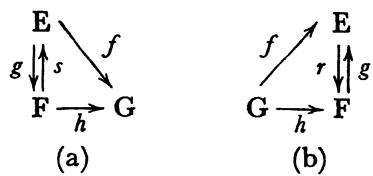
\includegraphics[keepaspectratio]{images/part001_ef8e01c05a3dcb28772fb1963be4c012627d42ff76089463ce60c193ac31650a.jpg}}

\begin{enumerate}
\def\labelenumi{(\alph{enumi})}
\setcounter{enumi}{1}
\item
  设E、F、G为集合，设g为F到E的一个单射，并设f为G到E的一个映射。则存在G到F的一个映射h，使得 \(f = g \circ h\) 当且仅当 \(f(\mathbf{G}) \subset f(\mathbf{F})\) 映射 h 由 f 唯一确定；若 r 是 g 的一个收缩，则我们有 \(h = r \circ f\) .
\item
  如果 \(f = h \circ g\) ，关系 \(g(x) = g(y)\) （其中 \(x \in \mathbf{E}\) , \(y \in \mathbf{E}\) ) 显然蕴含 \(f(x) = f(y)\) 。并且对于每个截面 \(s\) 的 \(g\) 我们拥有
\end{enumerate}

\[
h = h \circ (g \circ s) = f \circ s,
\]

，这表明 h 由 f 唯一确定。反之，假设关系 \(g(x) = g(y)\) 蕴含 \(f(x) = f(y)\) ；设 s 是 \(g\) 的一个截面，并令 \(h = f \circ s\) ；则对每个 \(x \in \mathbf{E}\) 都有 \(g(s(g(x))) = g(x)\) ，因而 \(f(s(g(x))) = f(x)\) ，即 \(h(g(x)) = f(x)\) 。因此 \(f = h \circ g\) .

\begin{enumerate}
\def\labelenumi{(\alph{enumi})}
\setcounter{enumi}{1}
\tightlist
\item
  如果 \(f = g \circ h\) ，那么显然 \(f(\mathbf{G}) \subset f(\mathbf{F})\) ，并且对于每个收缩 \(r\) 的 \(g\) 我们拥有 \(h = (r \circ g) \circ h = r \circ f\) ，这表明 \(h\) 由...唯一确定 \(f\) 相反，假设 \(f(\mathbf{G}) \subset f(\mathbf{F})\) ；令 \(r\) 为 \(g\) ，并放置 \(h = r \circ f\) ；对于每一个 \(x \in \mathbf{G}\) , 存在 \(y \in \mathbf{F}\) 使得 \(f(x) = g(y)\) ，因此
\end{enumerate}

\[
g (h (x)) = g (r (f (x))) = g (r (g (y))) = g (y) = f (x)
\]

因此 \(f = g \circ h\) .

\subsection{双自变量函数}

二元函数是指其定义域为有序对集合（或等价地，为某个乘积的子集）的函数。设 \(f\) 是这样一个函数；如果 \((x, y)\) 是定义域中的一个元素 \(f\) ，其值 \(f((x, y))\) 的 \(f\) 在元素 \((x, y)\) 通常用 \(f(x, y)\) . 设 \(f\) 是两个变量的函数， \(D\) 其定义域，以及 \(C\) 其陪域。对于每个 \(y\) 让 \(A_y\) 是所有……的集合 \(x\) 使得 \((x, y) \in D\) （即 \(\overline{D}^1\) 在 \(y\) （第1号）的截面）。映射

\[
x \rightarrow f (x, y) \quad (x \in \mathrm{A} _ {y}, f (x, y) \in \mathrm{C})
\]

称为由 \(f\) 关于第二个参数的取值 \(y\) 所定义的偏映射，并记为 \(f(\bullet, y)\) ，或 \(f(., y)\) 的复合（有时也称为 \(f_y\) ）；我们有 \(f(\bullet, y)(x) = f(x, y)\) 对于所有 \((x, y) \in D\) . 类似地，对于每一个 \(x\) 让 \(B_x\) 是所有……的集合 \(y\) 使得 \((x, y) \in D\) . 映射

\[
y \rightarrow f (x, y) \quad (y \in \mathbf {B} _ {x}, f (x, y) \in \mathbf {C})
\]

称为由 \(f\) 关于第二个参数的取值 \(x\) 关于第一个参数的取值，并记为 \(f(x, \bullet)\) ，或 \(f(x, \cdot)\) 的复合（有时也称为 \(f_x\) ）；我们有 \(f(x, \bullet)(y) = f(x, y)\) 对于所有 \((x, y) \in \mathbf{D}\) 。如果对每个 \(y\) （分别） \(x\) )，偏映射 \(f(\bullet, y)\) （分别） \(f(x, \bullet)\) )是常值映射，则称 \(f\) 不依赖于其第一个（分别地，第二个）参数；这意味着因此 \(f(x, y) = f(x', y)\) 每当 \((x, y)\) 并且 \((x', y)\) 属于 \(\mathbf{D}\) （分别） \(f(x, y) = f(x, y')\) 每当 \((x, y)\) 并且 \((x, y')\) 属于 \(\mathbf{D}\) ). 对于每一个 \(y\) 属于 \(\mathbf{D}\) 让 \(g(y)\) 表示其公共值 \(f(x, y)\) 为了 \(x \in A_y\) ；该映射 \(y \to g(y)\) 那么就是一个映射， \(\mathrm{pr}_2\mathbf{D}\) 进入。 \(\mathbf{C}\) 使得

\[
g (y) = f (x, y) \quad \text {   对   所有   } (x, y) \in D.
\]

反之，设 \(g\) 是集合 \(B\) 到集合 \(C\) 的一个映射，并设 \(A\) 为任意集合。则映射 \((x, y) \to g(y)\) （从 \(A \times B\) 到 \(C\) ）不依赖于第一个参数。

让 \(u\) 是A到C的一个映射，而 \(v\) B到D的一个映射。映射 \(z \to (u(\mathrm{pr}_1z), v(\mathrm{pr}_2z))\) 的 \(A \times B\) 进入。 \(C \times D\) 被称为 \(u\) 并且 \(v\) 到乘积集的（典范）扩张，或简称为 \(u\) 并且 \(v\) （若无混淆风险）；其值域为 \(u\langle A\rangle \times v\langle B\rangle\) 。它记作 \(u \times v\) 。如果 \(u\) 并且 \(v\) 是单射（相应地，满射），则 \(u \times v\) 是单射（相应地，满射）。如果 \(u\) 并且 \(v\) 若它们是双射的，则 \(u \times v\) 是双射的，且其逆映射为 \(\overline{u}^1 \times \overline{v}^1\) 。如果 \(u'\) 是将C映射到集合E的映射，并且如果 \(v'\) 是D到集合F的一个映射，我们有

\[
\left(u ^ {\prime} \times v ^ {\prime}\right) \circ (u \times v) = \left(u ^ {\prime} \circ u\right) \times \left(v ^ {\prime} \circ v\right).
\]

如果U、V分别是u、v的图像，那么W的图像 \(u \times v\) 是序对的集合 \(((x, y), (z, t))\) 的 \((\mathbf{A} \times \mathbf{B}) \times (\mathbf{C} \times \mathbf{D})\) 使得 \((x, z) \in \mathbf{U}\) 并且 \((y, t) \in \mathbf{V}\) ；该映射 \(((x, y), (z, t)) \to ((x, z), (y, t))\) 将W与乘积建立一一对应关系 \(U \times V\) （的一个子集 \((\mathbf{A} \times \mathbf{C}) \times (\mathbf{B} \times \mathbf{D})\) （参见§5，第5节）。

\section{一族集合的并集与交集}

\subsection{一族集合的并集与交集的定义}

设 X 是一个族（§3，第4号），I 是其指标集。为了便于对下文进行直观理解，我们将 X 称为一个集合族。若 (X, I, G) 是某个集合 E 的子集族（即其目标 G 满足关系 Y ∈ G 蕴含 Y ⊂ E），则我们将该族记为 (X\_t)\_\{t ∈ I\}(X\_t ∈ G) 或简记为 (X\_t)\_\{t ∈ I\} (§3, 第6节)；为简便起见，我们将任何以 I 为指标集的集合族记为 (X\_t)\_\{t ∈ I\}.

由于关系 \((\forall x)((\iota \in I\) 并且 \(x\in X_{\iota})\Longrightarrow (x\in X_{\iota}))\) 是真的，根据S5（第一章，§4，第2节）可知，该关系

\[
(\forall \iota) (\exists Z) (\forall x) ((\iota \in I \text { 且 } x \in X _ {\iota}) \Longrightarrow (x \in Z))
\]

是真的。根据方案S8（§1，第6节），关系 \((\exists t)(t \in I\) 并且 \(x \in X_t)\) 关于 \(x\) 是集合化的.

定义1. 设 \((\mathbf{X}_i)_{i\in I}\) 设为一个集合族（相应地，为集合E的子集族）。集合 \(\mathcal{E}_x((\exists i)(i\in I\) 并且 \(x\in \mathbf{X}_i))\) ，也就是说，所有 \(x\) 属于该族中至少一个集合的 \((\mathbf{X}_{\iota})_{\iota \in \mathbf{I}}\) ，称为该族的并集，记作 \(\bigcup \mathbf{X}_{\iota}(*)\) .

如果 \((\mathbf{X}_t)_{i\in I}\) 是集合的子集族 \(E\) ，则其并集是……的子集 \(E\) ; 注意它并不依赖于 \(E\) ，也不依赖于目标 \(\mathfrak{G}\) 该映射的 \(t\to X_t\) .

显然，如果 \(\mathbf{I} = \emptyset\) ，我们有 \(\bigcup_{i \in \mathbf{I}} \mathbf{X}_i = \emptyset\) 的集合，因为关系 \((\exists i)(i \in \mathbf{I}\) 并且 \(x \in \mathbf{X}_i)\) 此时为假。

现在假设 \(I \neq \varnothing\) 。如果 \(\alpha\) 是 I 的一个元素，关系

\[
(\forall \iota) ((\iota \in I) \Longrightarrow (x \in X _ {\iota}))
\]

蕴含 \(x \in \mathbf{X}_{\alpha}\) 。因此，根据 C52（§1，第 6 节），此关系关于 \(x\) 是集合化的。

定义 2. 设 \((\mathbf{X}_{\iota})_{\iota \in \mathbf{I}}\) 是一个集合族，其指标集 I 非空。集合 \(\mathcal{E}_x((\forall \iota)((\iota \in \mathbf{I}) \Longrightarrow (x \in \mathbf{X}_{\iota}))\) ，也就是说，所有 \(x\) 它属于该族中的每一个集合 \((\mathbf{X}_{\iota})_{\iota \in \mathbf{I}}\) ，称为该族的交集，记作 \(\bigcap_{\iota} \mathbf{X}_{\iota}\) .

如果 \(I = \varnothing\) ，关系 \((\forall t)((t \in I) \Longrightarrow (x \in X_t))\) 并未在 \(x\) ；因为这是一个真实的关系，且不存在这样的集合。 \(Y\) 使得 \(x \in Y\) 是一个真关系，因为 \(Y\) 则将是所有对象的集合（参见§1，第7号，注记）。

如果 \((\mathbf{X}_t)_{t \in \mathbf{I}}\) 是集合的子集族 \(E\) 并且如果 \(I \neq \emptyset\) ，关系“ \(x \in E\) 并且 \((\forall t)((t \in I) \Longrightarrow (x \in X_t))\) 等价于

\[
(\forall \iota) ((\iota \in I) \Longrightarrow (x \in X _ {\iota}));
\]

因此它在 \(x\) 中是集体化的，并且所有满足此关系的 \(x\) 的集合等于 \(\bigcap_{i \in I} X_i\) 。如果 \(I = \emptyset\) ，关系“ \(x \in E\) 并且 \((\forall i)((i \in I) \Longrightarrow (x \in X_i))\) ”等价于 \(x \in E\) ；因此它在 \(x\) 中是集体化的，并且所有满足此关系的 \(x\) 满足此关系的 \(E\) 因此，我们可以给出如下定义：

定义3。设 \((\mathbf{X}_{\iota})_{\iota \in \mathbf{I}}\) 设E是一个集合，E的子集族。集合

\[
\mathcal {E} _ {x} (x \in \mathrm{E} \text {   且   } (\forall \iota) ((\iota \in \mathrm{I}) \Longrightarrow (x \in \mathrm{X} _ {\iota}))),
\]

换言之，所有 \(x\) （属于 \(\mathbf{E}\) 且属于每个集合 \(\mathbf{X}_t\) ）所成的集合，称为该族的交集，记作 \(\bigcap_{i=1}^{\infty} \mathbf{X}_t\) .

因此，对于 \((\mathbf{X}_{i})_{i\in\theta}\) 的一个子集族，我们有

\[
\bigcap_ {i \in \theta} X _ {i} = E.
\]

但对于 \((\mathbf{X}_t)_{i\in I}\) 的一个子集族，若其指标集非空，则交集 \(\bigcap_{i\in I}\mathbf{X}_t\) 既不依赖于E，也不依赖于 \(\iota \to \mathbf{X}_t\) ；这证明了在定义2和定义3中使用相同记号的合理性。

命题1. 设 \((\mathbf{X}_{\mathfrak{t}})_{\mathfrak{t}\in \mathbf{I}}\) 是一族集合，并设 \(f\) 是从集合K到I的一个映射。则

\[
\bigcup_ {x \in \mathbf {K}} X _ {f (x)} = \bigcup_ {i \in I} X _ {i},
\]

并且，如果 \(\mathbf{I} \neq \emptyset\) ,

\[
\bigcap_ {x \in K} X _ {f (x)} = \bigcap_ {i \in I} X _ {i}.
\]

让 \(x\) 为 \(\bigcap_{i \in I} X_i\) . 存在一个指标 \(i \in I\) 使得 \(x \in X_i\) 。由于 \(f\langle K \rangle = I\) ，存在一个指标 \(x \in K\) 使得 \(i = f(x)\) ，由此 \(x \in X_{f(x)}\) ，从而

\[
x \in \bigcup_ {x \in \mathbf {K}} X _ {f (x)}.
\]

反之，如果 \(x \in \bigcup_{x \in \mathbb{K}} X_{f(x)}\) , 存在 \(x \in \mathbb{K}\) 使得 \(x \in X_{f(x)}\) ，因此，由于 \(f(x) \in I\) , \(x \in \bigcup_{i' \in I} X_i\) 。因此

\[
\bigcup_ {x \in \mathbb {K}} X _ {f (x)} = \bigcup_ {i \in I} X _ {i}.
\]

现在假设 \(\mathbf{I} \neq \emptyset\) ，并且让 \(x\) 为 \(\bigcap_{i \in \mathbf{I}} \mathbf{X}_i\) 。对于每个元素 \(x\) 的 \(\mathbf{K}\) 我们拥有 \(f(x) \in \mathbf{I}\) ，因此 \(x \in \mathbf{X}_{f(x)}\) ，从而

\[
x \in \bigcap_ {x \in \mathbb {K}} X _ {f (x)}.
\]

反之，设 \(x\) 为 \(\bigcap_{x \in \mathbf{K}} X_{f(x)}\) 。如果 \(\iota\) 是……的任意元素 \(I\) ，存在一个元素 \(x\) 的 \(K\) 使得 \(\iota = f(x)\) ，由此 \(x \in X_t\) 并且

因此 \(x \in \bigcap_{i \in I} X_i\) 。因此

\[
\bigcap_ {x \in \mathbf {K}} X _ {f (x)} = \bigcap_ {i \in I} X _ {i}.
\]

对于给定集合的子集族，命题1的第二部分显然在去掉限制后仍然成立。 \(I \neq \emptyset\) .

推论。设 \((\mathbf{X}_t)_{i\in \mathbf{I}}\) 设为一个集合族，使得 \(\mathbf{X}_t = \mathbf{X}_x\) 对于每一对索引 \((\mathfrak{t},\mathfrak{x})\) 然后对每一个 \(\alpha \in \mathbf{I}\) 我们拥有

\[
\bigcup_ {i \in I} X _ {i} = X _ {\alpha}, \quad \text{且} (\text{若 } I \neq \varnothing) \quad \bigcap_ {i \in I} X _ {i} = X _ {\alpha}.
\]

将命题1应用于常值映射 \(\iota\to\alpha\) 的 I 到 \(\{\alpha\}\) .

定义4. 设 \(\mathfrak{F}\) 是一组集合的集合，令 \(\Phi\) 是由恒等映射定义的集合族 \(\mathfrak{F}\) 这些集合的并集 \(\Phi\) 并且（如果 \(\mathfrak{F}\) （非空时）这些集合的交集 \(\Phi\) 分别称为集合族的并集和交集 \(\mathfrak{F}\) ，并记作 \(\bigcup_{X\sim X^{\prime}}X\) 并且 \(\bigcap_{X\sim X^{\prime}}X\) .

由命题1立即得出，如果 \((\mathbf{X}_i)_{i\in I}\) 是一个集合族，那么并集以及（若 \(I\neq \emptyset\) ) 该族的交集分别等于此族元素集合的并集与交集。

\subsection{并集与交集的性质}

如果 \((\mathbf{X}_t)_{t\in \mathbf{I}}\) 并且 \((\mathbf{Y}_t)_{t\in \mathbf{I}}\) 是具有相同指标集的集合族 \(\mathbf{I}\) ，并且如果 \(\mathbf{Y}_t\subset \mathbf{X}_t\) 对于每一个 \(t\in \mathbf{I}\) 那么显然

\[
\bigcup_ {i \in I} Y _ {i} \subset \bigcup_ {i \in I} X _ {i}, \quad \text { 且 } (\text { 若   } I \neq \emptyset) \quad \bigcap_ {i \in I} Y _ {i} \subset \bigcap_ {i \in I} X _ {i}.
\]

让 \((\mathbf{X}_t)_{t\in \mathbf{I}}\) 设为一个集合族。若 \(J\subset I\) ，我们有

\[
\bigcup_ {i \in J} X _ {i} \subset \bigcup_ {i \in I} X _ {i}, \quad \text { 且 } (\text { 若 } J \neq \emptyset) \quad \bigcap_ {i \in J} X _ {i} \supset \bigcap_ {i \in I} X _ {i}.
\]

命题2. 设 \((\mathbf{X}_{\iota})_{\iota \in \mathbf{I}}\) 为一个集合族，其指标集 I 是某个族 \((\mathrm{J}_{\lambda})_{\lambda \in \mathbf{L}}\) 的并集。则

\[
\bigcup_ {i \in I} X _ {i} = \bigcup_ {\lambda \in L} \left(\bigcup_ {i \in J _ {\lambda}} X _ {i}\right),
\]

并且（如果 \(\mathbf{L} \neq \phi\) 并且 \(J_{\lambda} \neq \phi\) 对于每一个 \(\lambda \in \mathbf{L}\) )

\[
\bigcap_ {i \in I} X _ {i} = \bigcap_ {\lambda \in L} \left(\bigcap_ {i \in J _ {\lambda}} X _ {i}\right)
\]

（并集与交集的“结合律”）。

让 \(x\) 为 \(\bigcup_{i \in I} X_i\) . 存在一个指标 \(i \in I\) 使得 \(x \in X_i\) 。由于 \(I\) 是族 \((J_\lambda)_{\lambda \in L}\) ，存在一个指标 \(\lambda \in L\) 使得 \(i \in J_\lambda\) ，由此 \(x \in \bigcup X_i\) ，并且因此

\[
x \in \bigcup_ {\lambda \in L} \left(\bigcup_ {i \in J _ {\lambda}} X _ {i}\right).
\]

反之，设 \(x\) 是此集合的一个元素。存在一个指标 \(\lambda \in L\) 使得 \(x \in \bigcup_{\iota \in J_{\lambda}} X_{\iota}\) ，因此存在一个指标 \(\iota \in J_{\lambda}\) （从而 \(\iota \in I\) ) 使得 \(x \in X_{\iota}\) ；由此得出

\[
x \in \bigcup_ {i \in I} X _ {i}.
\]

现在假设 \(L \neq \emptyset\) 并且 \(J_{\lambda} \neq \emptyset\) 对于每一个 \(\lambda \in L\) 。然后 \(I \neq \emptyset\) 。设 x 为 \(\bigcap_{i \in I} X_{i}\) 。如果 \(\lambda \in L\) ，我们有 \(x \in X_{i}\) 对于每一个 \(i \in J_{\lambda}\) （因为 \(J_{\lambda} \subset I\) ），所以 \(x \in \bigcap_{i \in J_{\lambda}} X_{i}\) 。由于最后的包含关系对所有 \(\lambda \in L\) ，x 属于 \(\bigcap_{\lambda \in L} \left( \bigcap_{i \in J_{\lambda}} X_{i} \right)\) 。反之，设 x 是后一个集合的元素，并设 i 是 I 的任意元素。存在 \(\lambda \in L\) 使得 \(i \in J_{\lambda}\) ；由于 \(x \in \bigcap_{i \in J_{\lambda}} X_{i}\) ，我们有 \(x \in X_{i}\) ，这对所有 \(i \in I\) 。因此 \(x \in \bigcap_{i \in I} X_{i}\) 都成立。这就完成了证明。

对于给定集合的子集族，命题2的第二部分在不对L作限制的情况下仍然成立，且 \(J_{\lambda}\) .

\subsection{并集与交集的像}

命题3。设 \((\mathbf{X}_t)_{t\in I}\) 是集合A的子集族，并设 \(\Gamma\) 是A与B之间的对应关系。则

\[
\Gamma \left\langle \bigcup_ {i \in I} X _ {i} \right\rangle = \bigcup_ {i \in I} \Gamma \left\langle X _ {i} \right\rangle , \quad \Gamma \left\langle \bigcap_ {i \in I} X _ {i} \right\rangle \subset \bigcap_ {i \in I} \Gamma \left\langle X _ {i} \right\rangle .
\]

关系 \((\exists x)\left(x\in \bigcup_{i\in I}X_i \text{ 且 } y\in \Gamma (x)\right)\) 等价于

\[
(\exists x) (\exists t) (t \in I \text {   且   } x \in X _ {t} \text {   且   } y \in \Gamma (x)),
\]

因此到 \((\exists \iota)(\iota \in I \text{ 且 } y \in \Gamma\langle X_{\iota}\rangle)\) ，因此等价于 \(y \in \bigcup_{\iota \in I} \Gamma\langle X_{\iota}\rangle\) ；这证明了第一个公式。至于第二个公式，我们有 \(\bigcap_{\iota \in I} X_{\iota} \subset X_{\iota}\) 对于所有 \(\iota \in I\) ，由此（§3，命题2）

\[
\Gamma \left\langle \bigcap_ {i \in I} X _ {i} \right\rangle \subset \Gamma \left\langle X _ {i} \right\rangle ,
\]

，从而

\[
\Gamma \left\langle \bigcap_ {i \in I} X _ {i} \right\rangle \subset \bigcap_ {i \in I} \Gamma \left\langle X _ {i} \right\rangle .
\]

如果 \(\Gamma\) 是任意对应关系（特别是任意函数），公式

\[
\Gamma \left\langle \bigcap_ {i \in I} X _ {i} \right\rangle = \bigcap_ {i \in I} \Gamma \left\langle X _ {i} \right\rangle
\]

通常不成立。

* 例如，在平面中 \(\mathbf{R}^2\) 这些直线的第一投影 \(y = x\) 并且 \(y = x + 1\) 等于 \(\mathbf{R}\) , 但这些直线的交集为空，因此该交集的第一投影也为空 (*)。*

然而，我们有以下重要结果：

命题4。设 \(f\) 设 为从 A 到 B 的映射，并设 \((\mathbf{Y}_t)_{t \in I}\) 为 B 的子集族。则 \(\overline{f}^1 \left\langle \bigcap_{i \in I} \mathbf{Y}_t \right\rangle = \bigcap_{i \in I} \overline{f}^1 \langle \mathbf{Y}_t \rangle\) .

为证明这一点，设 \(x\) 为 \(\bigcap_{i \in I} f^{-1} \langle Y_i \rangle\) 我们有 \(f(x) \in Y_i\) 对于所有 \(i \in I\) ，由此 \(f(x) \in \bigcap_{i \in I} Y_i\) ，并且因此

\[
x \in \overline {{f}} ^ {1} \left\langle \bigcap_ {\iota \in I} Y _ {\iota} \right\rangle .
\]

因此 \(\bigcap_{i\in I}\overline{f}^{1}(Y_{i})\subset\overline{f}^{1}\Big\langle\bigcap_{i\in I}Y_{i}\Big\rangle\) ；这一关系，连同命题3，给出了结果。

推论. 如果 \(f\) 是从 \(A\) 到 \(B\) 的单射，且 \((X_{t})_{t \in I}\) 是 \(A\) 的子集族，其指标集 \(I\) 非空，则 \(f\left\langle \bigcap_{i \in I} X_{t} \right\rangle = \bigcap_{i \in I} f\langle X_{t} \rangle\) .

因为可写成 \(f = i \circ g\) ，其中 \(i\) 是从 \(f\langle \mathbf{A} \rangle\) 到 \(\mathbf{B}\) 的典范单射，而 \(g\) 是从 \(\mathbf{A}\) 到 \(f\langle \mathbf{A} \rangle\) 的双射。如果 \(h\) 表示 \(g\) 的逆映射，则我们有 \(f\langle \mathbf{X} \rangle = \overline{h}^1\langle \mathbf{X} \rangle\) ，其中 \(\mathbf{X}\) 是 \(\mathbf{A}\) 的任意子集，因而归结为命题4。

\subsection{并集与交集的补集}

命题5。对于每一个族 \((\mathbf{X}_t)_{t\in I}\) 对于集合E的子集族，我们有

\[
\mathbb {G} _ {\mathrm{E}} \left(\bigcup_ {i \in \mathrm{I}} \mathrm{X} _ {i}\right) = \bigcap_ {i \in \mathrm{I}} \left(\mathbb {G} _ {\mathrm{E}} \mathrm{X} _ {i}\right), \quad \mathbb {G} _ {\mathrm{E}} \left(\bigcap_ {i \in \mathrm{I}} \mathrm{X} _ {i}\right) = \bigcup_ {i \in \mathrm{I}} \left(\mathbb {G} _ {\mathrm{E}} \mathrm{X} _ {i}\right).
\]

让 \(x \in \complement_{\mathbf{E}} \left( \bigcup_{i \in \mathbf{I}} \mathbf{X}_i \right)\) 。然后 \(x \in E\) 并且，对于每一个 \(i \in I\) , \(x \notin \mathbf{X}_i\) ，因此 \(x \in \complement_{\mathbf{E}} \mathbf{X}_i\) ；因此

\[
x \in \bigcap_ {i \in I} \left(\complement_ {E} X _ {i}\right).
\]

反之，设 \(x\) 为 \(\bigcap_{i \in I} (\complement_E X_i)\) ；根据交的定义，我们有 \(x \in E\) 。此外，如果我们有 \(x \in \bigcup_{i \in I} X_i\) ，那么将存在一个指标 \(x \in I\) 使得 \(x \in X_x\) ，这与假设相矛盾 \(x \in \bigcap_{i \in I} (\complement_E X_i)\) ；因此

\[
x \in \mathbb {C} _ {\mathbf {E}} \left(\bigcup_ {i \in \mathbf {I}} \mathrm{X} _ {i}\right).
\]

这证明了第一个公式；第二个公式是直接推论，鉴于关系式 \(\mathbf{G}_{\mathbf{E}}(\mathbf{G}_{\mathbf{E}}\mathbf{X})=\mathbf{X}\) 对 E 的每个子集 X 成立。

\subsection{两个集合的并集与交集}

若 A、B 是集合，我们记

\[
\mathrm{A} \cup \mathrm{B} = \bigcup_ {\mathbf {X} \in \{\mathbf {A}, \mathrm{B} \}} \mathrm{X}, \quad \mathrm{A} \cap \mathrm{B} = \bigcap_ {\mathbf {X} \in \{\mathbf {A}, \mathrm{B} \}} \mathrm{X}.
\]

显然，A ∪ B 是所有属于 A 或属于 B（或同时属于两者）的对象的集合，而 A ∩ B 是所有同时属于 A 和 B 的对象的集合。特别地， \{x, y\} = \{x\} ∪ \{y\}. 设 \{x, y, z\} = \{x, y\} ∪ \{z\}。集合 \{x, y, z\} 是仅以 x、y 和 z 为元素的集合。类似地，我们写

\[
\{x, y, z, t \} = \{x, y, z \} \cup \{t \},
\]

等等。

如果 A、B、C、D 是集合，我们写

\[
\begin{array}{c} \mathrm {A \cup B \cup C = \bigcup_ {\mathbf {X} \in \{\mathrm{A,B,C} \}} X, \quad A \cap B \cap C = \bigcap_ {\mathbf {X} \in \{\mathrm{A,B,C} \}} X;} \\ \mathrm {A \cup B \cup C \cup D = \bigcup_ {\mathbf {X} \in \{\mathrm{A,B,C,D} \}} X, \quad A \cap B \cap C \cap D = \bigcap_ {\mathbf {X} \in \{\mathrm{A,B,C,D} \}} X;} \end{array}
\]

等等。

设 A、B、C 是集合。由命题 1 和命题 2 我们推出公式

\[
\begin{array}{c} \mathbf {A} \cup \mathbf {B} = \mathbf {B} \cup \mathbf {A}, \qquad \mathbf {A} \cap \mathbf {B} = \mathbf {B} \cap \mathbf {A}, \\ \mathbf {A} \cup (\mathbf {B} \cup \mathbf {C}) = (\mathbf {A} \cup \mathbf {B}) \cup \mathbf {C} = \mathbf {A} \cup \mathbf {B} \cup \mathbf {C}, \\ \mathbf {A} \cap (\mathbf {B} \cap \mathbf {C}) = (\mathbf {A} \cap \mathbf {B}) \cap \mathbf {C} = \mathbf {A} \cap \mathbf {B} \cap \mathbf {C}. \end{array}
\]

这些公式也是准则 C24（第一章，§3，第 5 号）中所陈述定理的直接推论。类似地，可以证明公式

\[
\mathbf {A} \cup (\mathbf {B} \cap \mathbf {C}) = (\mathbf {A} \cup \mathbf {B}) \cap (\mathbf {A} \cup \mathbf {C}), \quad \mathbf {A} \cap (\mathbf {B} \cup \mathbf {C}) = (\mathbf {A} \cap \mathbf {B}) \cup (\mathbf {A} \cap \mathbf {C})
\]

（并关于交的“分配律”以及交关于并的分配律；参见 §5，第 6 号）。

关系 \(\mathbf{A} \subset \mathbf{B}\) 等价于 \(\mathbf{A} \cup \mathbf{B} = \mathbf{B}\) 以及 \(\mathbf{A} \cap \mathbf{B} = \mathbf{A}\) 。如果 \(\mathbf{A}\) 和 \(\mathbf{B}\) 是集合 \(\mathbf{E}\) 的子集，我们从命题5（或从准则C24）推导出公式

\[
\mathbb {G} _ {\mathbf {E}} (\mathbf {A} \cup \mathbf {B}) = \left(\mathbb {G} _ {\mathbf {E}} \mathbf {A}\right) \cap \left(\mathbb {G} _ {\mathbf {E}} \mathbf {B}\right), \quad \mathbb {G} _ {\mathbf {E}} (\mathbf {A} \cap \mathbf {B}) = \left(\mathbb {G} _ {\mathbf {E}} \mathbf {A}\right) \cup \left(\mathbb {G} _ {\mathbf {E}} \mathbf {B}\right);
\]

此外，我们有

\[
\mathrm{A} \cup (\mathbb {C} _ {\mathrm{E}} \mathrm{A}) = \mathrm{E}, \quad \mathrm{A} \cap (\mathbb {C} _ {\mathrm{E}} \mathrm{A}) = \varnothing .
\]

如果 \(\Gamma\) 是...之间的对应关系 \(E\) 并且 \(F\) ，并且如果 \(A, B\) 是……的子集 \(E\) ，由命题3可知

\[
\Gamma \langle \mathrm{A} \cup \mathrm{B} \rangle = \Gamma \langle \mathrm{A} \rangle \cup \Gamma \langle \mathrm{B} \rangle , \quad \Gamma \langle \mathrm{A} \cap \mathrm{B} \rangle \subset \Gamma \langle \mathrm{A} \rangle \cap \Gamma \langle \mathrm{B} \rangle ,
\]

并且，如果 \(f\) 是从 \(F\) 到 \(E\) 的映射，

\[
\overline {{{f}}} ^ {1} \langle \mathrm{A} \cap \mathrm{B} \rangle = \overline {{{f}}} ^ {1} \langle \mathrm{A} \rangle \cap \overline {{{f}}} ^ {1} \langle \mathrm{B} \rangle
\]

由命题4得出。

我们还记录以下关于补集的命题：

命题6. 设 \(f\) 是从 \(A\) 到 \(B\) 的映射。对于 \(B\) 的每一个子集 \(Y\) ，都有

\[
\overline {{{f}}} ^ {1} \langle \mathrm{B} - \mathrm{Y} \rangle = \overline {{{f}}} ^ {1} \langle \mathrm{B} \rangle - \overline {{{f}}} ^ {1} \langle \mathrm{Y} \rangle .
\]

因为 \(x\) 属于 \(\overline{f}^1\langle \mathbf{B} - \mathbf{Y}\rangle\) 当且仅当 \(f(x)\) 属于 \(\mathbf{B}\) 而不属于 \(\mathbf{Y}\) ，也就是当且仅当 \(x\) 属于 \(\overline{f}^1\langle \mathbf{B}\rangle\) 而不属于 \(\overline{f}^1\langle \mathbf{Y}\rangle\) .

推论。设 \(f\) 是从 \(\mathbf{A}\) 到 \(\mathbf{B}\) 的单射。对于 \(\mathbf{A}\) 的每一个子集 \(\mathbf{X}\) ，都有 \(f\langle \mathbf{A} - \mathbf{X}\rangle = f\langle \mathbf{A}\rangle - f\langle \mathbf{X}\rangle\) .

写成 \(f = i \circ g\) ，其中 \(i\) 是从 \(f\langle A\rangle\) 到 B 的典范单射，就把该推论化归为对 \(\overline{g}^1\) 应用命题6。

¶ 交集 X ∩ A 有时称为 X 在 A 上的迹。若 F 是一个集合族，则 F 中集合在 A 上的迹所组成的集合称为 F 在 A 上的迹。

\subsection{覆盖}

定义5. 一个集合族 \((\mathbf{X}_t)_{t \in I}\) 称为集合 E 的一个覆盖（或覆盖 E），如果 \(\mathbf{E} \subset \bigcup_{i \in I} \mathbf{X}_t\) 。如果 \((\mathbf{X}_t)_{t \in I}\) 并且 \((\mathbf{Y}_x)_{x \in K}\) 是 E 的覆盖，则这些覆盖中的第二个被称为比第一个更细（或称为第一个的加细，或加细第一个），如果对每个 \(x \in K\) , 存在 \(t \in I\) 使得

\[
\mathrm{Y} _ {x} \subset \mathrm{X} _ {i}.
\]

一个集合族 \(\Re\) 是 \(E\) 如果由恒等映射定义的集合族 \(\Re\) 是 \(E\) ，换言之，如果 \(E \subset \bigcup_{X \in \mathbb{R}} X\) .

如果 \(\Re\) , \(\Re'\) , \(\Re''\) 是E的三个覆盖，使得 \(\Re'\) 加细 \(\Re\) 并且 \(\Re''\) 加细 \(\Re'\) ，显然 \(\Re''\) 加细 \(\Re\) .

让 \((\mathbf{X}_t)_{i\in I}\) 是 E 的一个覆盖。若 J 是 I 的子集使得 \((\mathbf{X}_t)_{i\in J}\) 仍是 E 的一个覆盖，则此覆盖显然加细 \((\mathbf{X}_t)_{i\in I}\) .

让 \((\mathbf{X}_t)_{t \in I}\) 并且 \((\mathbf{Y}_x)_{x \in K}\) 是集合 \(E\) 的覆盖。则集合族 \((\mathbf{X}_t \cap \mathbf{Y}_x)_{(t,x) \in I \times K}\) 是 \(E\) 。因为如果 \(x \in E\) ，存在指标 \(t \in I\) 并且 \(x \in K\) 使得 \(x \in X_t\) 并且 \(x \in Y_x\) ，因此 \(x \in X_t \cap Y_x\) 。此外，显然覆盖 \((\mathbf{X}_t \cap Y_x)_{(t,x) \in I \times K}\) 加细每一个 \(o\) 覆盖 \((\mathbf{X}_t)_{i\in \mathbf{I}}, (\mathbf{Y}_x)_{x\in \mathbf{K}}\) 。反过来，设 \((\mathbf{Z}_{\lambda})_{\lambda \in \mathbf{L}}\) 是……的一个覆盖， \(\mathbf{E}\) 它细化每一个覆盖 \((\mathbf{X}_t)_{i\in \mathbf{I}}, (\mathbf{Y}_x)_{x\in \mathbf{K}}\) ；若 \(\lambda \in \mathbf{L}\) ，则存在指标 \(i\in \mathbf{I}\) 并且 \(x\in \mathbf{K}\) 使得 \(Z_{\lambda}\subset X_{i}\) 并且 \(Z_{\lambda}\subset Y_{x}\) ，因此 \(Z_{\lambda}\subset X_{i}\cap Y_{x}\) ；因此该覆盖 \((Z_{\lambda})_{\lambda \in \mathbf{L}}\) 是……的一个加细

\[
\left(\mathrm{X} _ {i} \cap \mathrm{Y} _ {x}\right) _ {(i, x) \in \mathrm{I} \times \mathrm{K}}.
\]

让 \((\mathbf{X}_t)_{t\in I}\) 是集合 A 的一个覆盖，并令 \(f\) 是A到集合B上的一个映射。族 \((f\langle \mathbf{X}_t\rangle)_{t\in I}\) 于是构成B的一个覆盖（命题3），称为在 \(f\) 覆盖的 \((\mathbf{X}_t)_{t\in I}\) 。如果 \(g\) 是将集合 C 映射到集合 A 的映射，该族 \((\overline{g}\langle \mathbf{X}_t\rangle)_{t\in I}\) 是C的一个覆盖，称为在 \(g\) 覆盖的 \((\mathbf{X}_t)_{t\in I}\) .

设E和F为集合，令 \((\mathbf{X}_t)_{i \in I}\) 是 E 的一个覆盖，并令 \((\mathbf{Y}_x)_{x \in K}\) 是F的一个覆盖。该族 \((\mathbf{X}_t \times \mathbf{Y}_x)_{(i,x) \in I \times K}\) 于是便是E × F的一个覆盖，称为覆盖 \((\mathbf{X}_t)_{i \in I}\) E与 \((\mathbf{Y}_x)_{x \in K}\) F的乘积。

命题7. (1) 设E是一个集合，且 \((\mathbf{X}_{\iota})_{\iota \in \mathbf{I}}\) 是E的一个覆盖。若 \(f\) 并且 \(g\) 是两个定义域为 E 的函数，使得 \(f\) 并且 \(g\) 在 \(\mathbf{E} \cap \mathbf{X}_{\iota}\) 对于每一个 \(\iota \in \mathbf{I}\) ，那么 \(f\) 并且 \(g\) 在 E 上一致。

\begin{enumerate}
\def\labelenumi{(\arabic{enumi})}
\setcounter{enumi}{1}
\item
  设 \((\mathbf{X}_i)_{i \in I}\) 是一族集合，且设 \((f_i)_{i \in I}\) 是同一目标 F 的一族映射，使得对每个 \(i \in I\) ， \(f_i\) 的定义域是 \(\mathbf{X}_i\) ，并且对于每一对 \((i, x) \in I \times I\) , \(f_i\) 和 \(f_x\) 在 \(\mathbf{X}_i \cap \mathbf{X}_x\) 上一致。那么恰好存在一个函数 \(f\) ，其定义域为 \(A = \bigcup_{i \in I} X_i\) ，目标为 F，并且它扩展了每一个函数 \(f_i (i \in I)\) .
\item
  设 \(x\) 为 \(\mathbf{E}\) 的任意元素。那么存在 \(t \in I\) 使得 \(x \in X_t\) ，由此 \(f(x) = g(x)\) 根据假设成立。
\item
  让 \(G_{i}\) 是 \(f_{i}\) 并令 \(G = \bigcup_{i \in I} G_{i}\) 的图；让我们证明 \(G\) 是一个函数图。如果 \((x, y) \in G\) 并且 \((x, y') \in G\) , 存在两个指标 \(i, x\) 在 \(I\) 使得 \((x, y) \in G_{i}\) 并且 \((x, y') \in G_{x}\) 。这意味着 \(x \in X_{i}, x \in X_{x}, y = f_{i}(x), y' = f_{x}(x)\) ；但由于 \(x \in X_{i} \cap X_{x}\) ，我们有
\end{enumerate}

\[
f _ {i} (x) = f _ {x} (x),
\]

也就是说， \(y = y'\) 。图 \(G\) 的定义域为 \(\mathrm{pr}_1 G = \bigcup_{i \in I} \mathrm{pr}_1 G_i = A\) ；因此函数 \(f = (G, A, F)\) 满足所需条件。其唯一性由命题的第一部分得出。

\subsection{划分}

定义6. 若集合A与B不相交（或不交），则称它们为不相交的（或不相交的）；若 \(\mathbf{A} \cap \mathbf{B} = \phi\) 。如果 \(\mathbf{A} \cap \mathbf{B} \neq \phi\) ，则称A与B相遇（或相交）。设 \((\mathbf{X}_{t})_{i \in I}\) 设为一个集合族。该族中的集合被称为互不相交的，如果满足条件 \(i \in I\) , \(x \in I\) , \(i \neq x\) 蕴含 \(\mathbf{X}_{t} \cap \mathbf{X}_{x} = \phi\) .

设 \(f\) 是从 \(\mathbf{A}\) 到 \(\mathbf{B}\) 的映射，并设 \((\mathbf{Y}_i)_{i\in \mathbf{I}}\) 是 \(\mathbf{B}\) 的一族两两不相交的子集。命题4表明， \((\overline{f}^1\langle \mathbf{Y}_i\rangle)_{i\in \mathbf{I}}\) （ \(\mathbf{A}\) 的子集族）中的各集合两两不相交。另一方面，如果 \((\mathbf{X}_i)_{i\in \mathbf{I}}\) 是 \(\mathbf{A}\) 的一族两两不相交的子集，则族 \((f\langle \mathbf{X}_i\rangle)_{i\in \mathbf{I}}\) 中的各集合一般并不两两不相交。

命题8. 设 \((\mathbf{X}_t)_{t \in I}\) 是一族互不相交的集合，且设 \((f_t)_{t \in I}\) 是定义域为 \(f_t\) 是 \(\mathbf{X}_t\) 对于每一个 \(t \in I\) 那么存在恰好一个函数 \(f\) ，其定义域为 \(\bigcup_{i \in I} \mathbf{X}_t\) ，目标为 F，并且它扩展了每一个函数 \(f_t\) ( \(t \in I\) ).

这是命题7的一个推论，因为 \(f_{\iota}\) 并且 \(f_{x}\) 显然在 \(\mathbf{X}_{\iota} \cap \mathbf{X}_{x} = \emptyset\) 每当 \(\iota \neq x\) .

定义7. 集合E的一个划分是E的非空互不相交子集的一个族，它们覆盖E。

例. 对于每个非空集合A，族 \((\{x\})_{x\in\mathbf{A}}\) 是A的一个划分。

如果 \((\mathbf{X}_i)_{i\in I}\) 是集合的一个划分 \(E\) ，映射 \(\iota \to X_i\) 的 \(I\) 到集合 \(\mathfrak{F}\) 的元素 \(X_i\) 的划分是双射的。因此，若 \(\mathfrak{F}\) 给定，则该划分在指标集之间的一一对应意义下是确定的。通常当我们谈到一个划分时，我们所关心的是划分中元素所构成的集合。

\subsection{集合族的并}

命题9. 设 \((\mathbf{X}_t)_{t \in I}\) 是一个集合族。则存在一个集合 \(\mathbf{X}\) ，具有如下性质： \(\mathbf{X}\) 是两两不相交集合族 \((\mathbf{X}_t')_{t \in I}\) 的并，并且对每个 \(t \in I\) 都存在一个从 \(\mathbf{X}_t\) 到 \(\mathbf{X}_t'\) 的单射。

让 \(A = \bigcup_{i \in I} X_i\) 。如果 \(i \in I\) ，映射 \(x \to (x, i)\) ( \(x \in X_i\) 是 \(X_i\) 到子集 \(X_i'\) 的 \(A \times I\) 。此外， \(X_i'\) 在第二个坐标函数下的像 \(A \times I\) 包含于集合 \(\{i\}\) ；由此得出 \(X_i' \cap X_x' = \emptyset\) 每当 \(i \neq x\) 。于是我们可以取 \(X = \bigcup_{i \in I} X_i'\) .

定义8. 设 \((\mathbf{X}_{\iota})_{\iota \in \mathbf{I}}\) 为一族集合。该族的和是这族集合的并集 \((\mathbf{X}_{\iota} \times \{\iota\})_{\iota \in \mathbf{I}}\) .

命题10。设 \((\mathbf{X}_t)_{t\in I}\) 设为一族互不相交的集合。设A为其并集，S为其和。则存在一个从A到S的双射映射。

对于每一个 \(t \in I\) ，令 \(f_{t}\) 为从 \(X_{t}\) 到 \(X_{t} \times \{t\}\) 的双射。根据命题8，存在一个从 A 到 S 的映射 f，它扩张所有映射 \(f_{t}\) 。立即可验证，f 是从 A 到 S 的双射。

滥用语言来说，集合 E 被称为一族集合的和 \((\mathbf{X}_{t})_{t\in\mathbf{I}}\) 若存在从E到该族之和的双射，如定义8中所定义的那样。

注意，如果 \((\mathbf{X}_{t})_{i\in\mathbf{I}}\) 若一族集合是任意的，命题10的论证表明存在一个从和S到并集A的映射。

\section{集合族的乘积}

\subsection{子集集合公理}

\[
(\forall \mathbf {X}) \operatorname{Coll} _ {\mathbf {Y}} (\mathbf {Y} \subset \mathbf {X}).
\]

该公理意味着，对于每个集合 X，存在一个集合，其元素是 X 的所有子集，即集合 \(\mathcal{E}_{\mathbf{Y}}(\mathbf{Y}\subset\mathbf{X})\) （§1，第4节）；该集合记为 \(\mathfrak{P}(\mathbf{X})\) 并被称为X的子集集合。显然，如果 \(X\subset X'\) ，我们有 \(\mathfrak{P}(\mathbf{X})\subset\mathfrak{P}(\mathbf{X}')\) .

设 A、B 为两个集合， \(\Gamma\) 为 A 与 B 之间的对应。函数 \(X \to \Gamma\langle X\rangle\) ( \(X \subset \mathfrak{P}(A)\) , \(\Gamma\langle X\rangle \in \mathfrak{P}(B)\) ) 称为 \(\Gamma\) 到子集集合上的典范扩张（或简称扩张），记作 \(\hat{\Gamma}\) ；它是从 \(\mathfrak{P}(A)\) 到 \(\mathfrak{P}(B)\) 的映射。如果 \(\Gamma'\) 是 B 与集合 C 之间的一个对应，则公式 \((\Gamma' \circ \Gamma)\langle X\rangle = \Gamma'\langle\Gamma\langle X\rangle\rangle\) 表明， \(\Gamma' \circ \Gamma\) 到子集集合上的扩张就是映射 \(\hat{\Gamma}' \circ \hat{\Gamma}\) .

命题1. (1) 若 \(f\) 是集合 \(\mathbf{E}\) 到集合 \(\mathbf{F}\) 的满射，则典范扩张 \(\hat{f}\) （ \(f\) 的）是从 \(\mathfrak{P}(\mathbf{E})\) 到 \(\mathfrak{P}(\mathbf{F})\) 的满射。

\begin{enumerate}
\def\labelenumi{(\arabic{enumi})}
\setcounter{enumi}{1}
\item
  如果 \(f\) 是从 \(\mathbf{E}\) 到 \(\mathbf{F}\) 的单射，则典范扩张 \(\hat{f}\) （ \(f\) 的）是从 \(\mathfrak{P}(\mathbf{E})\) 到 \(\mathfrak{P}(\mathbf{F})\) 的单射。
\item
  如果 \(s\) 是 \(f\) ，那么 \(f \circ s\) 是 \(\mathbf{F}\) ，因此 \(\hat{f} \circ \hat{s}\) 是 \(\mathfrak{P}(\mathbf{F})\) 中；因此 \(\hat{f}\) 是满射，且 \(\hat{s}\) 是 \(\hat{f}\) （§3，第8节）。
\item
  该命题在以下情形下是显然的： \(\mathbf{E} = \varnothing\) ，因为那样 \(\mathfrak{P}(\mathbf{E}) = \{\varnothing\}\) 。如果 \(\mathbf{E} \neq \varnothing\) 并且如果 \(r\) 是 \(f\) ，那么 \(r \circ f\) 是 \(\mathbf{E}\) ，因此 \(\hat{r} \circ \hat{f}\) 是 \(\mathfrak{P}(\mathbf{E})\) 中；因此 \(\hat{f}\) 是单射，并且 \(\hat{r}\) 是 \(\hat{f}\) （§3，第8节）。
\end{enumerate}

\subsection{一个集合到另一个集合的映射集}

设 E, F 为集合。从 E 到 F 的映射的图是 \(E \times F\) 的子集。因此， \(\mathfrak{P}(E \times F)\) 中由从 E 到 F 的映射的图所构成的元素集合，是 \(\mathfrak{P}(E \times F)\) 的一个子集，记为 \(F^{E}\) 。所有三元组 \(f = (G, E, F)\) （其中 \(G \in F^{E}\) ）所成的集合，就是从 E 到 F 的映射全体；它记为 \(\mathcal{F}(E, F)\) 。显然， \(G \to (G, E, F)\) 是从 \(F^{E}\) 到 \(\mathcal{F}(E, F)\) 的一个双射（称为典范双射）。这个双射使我们能够立即把关于集合 \(F^{E}\) 的每个命题转化为关于 \(\mathcal{F}(E, F)\) 的命题，反之亦然。

设 E、E'、F、F' 为集合。设 u 为从 E' 到 E 的映射，v 为从 F 到 F' 的映射。则函数 \(f \rightarrow v \circ f \circ u\) 是从 \(\mathcal{F}(\mathrm{E}, \mathrm{F})\) 到 \(\mathcal{F}(\mathrm{E}', \mathrm{F}')\) 的映射。

命题 2. (1) 若 \(u\) 是从 \(\mathbf{E}'\) 到 \(\mathbf{E}\) 的满射，而 \(v\) 是从 \(\mathbf{F}\) 到 \(\mathbf{F}'\) 的单射，则映射 \(f \to v \circ f \circ u\) 是单射。

\begin{enumerate}
\def\labelenumi{(\arabic{enumi})}
\setcounter{enumi}{1}
\tightlist
\item
  如果 \(u\) 是从 \(\mathbf{E}'\) 到 \(\mathbf{E}\) 的单射，而 \(v\) 是从 \(\mathbf{F}\) 到 \(\mathbf{F}'\) 的满射，则映射 \(f \to v \circ f \circ u\) 是满射。
\end{enumerate}

我们将假设集合 E、E'、F、F' 均为非空，否则命题显然成立。

\begin{enumerate}
\def\labelenumi{(\arabic{enumi})}
\tightlist
\item
  让 \(s\) 是……的一个截面 \(u\) 并令 \(r\) 为 \(v\) （§3，定义 11）。则 \(r \circ (v \circ f \circ u) \circ s = I_F \circ f \circ I_E = f\) ，因此
\end{enumerate}

\[
f \rightarrow v \circ f \circ u
\]

是单射的。

\begin{enumerate}
\def\labelenumi{(\arabic{enumi})}
\setcounter{enumi}{1}
\tightlist
\item
  让 \(r'\) 为 \(u\) 并令 \(s'\) 是……的一个截面 \(v\) 。对于每个映射 \(f': E' \to F'\) 我们拥有 \(v \circ (s' \circ f' \circ r') \circ u = f'\) ，这表明映射 \(f \to v \circ f \circ u\) 的满射。
\end{enumerate}

推论. 如果 \(u\) 是从 \(\mathbf{E}'\) 到 \(\mathbf{E}\) 的双射，且 \(v\) 是从 \(\mathbf{F}\) 到 \(\mathbf{F}'\) 的双射，那么 \(f \to v \circ f \circ u\) 是双射。

设 A、B、C 为三个集合，并设 f 为从 \(B \times C\) 到 A 的一个映射。对每一个 \(y \in C\) ，令 \(f(\bullet, y)\) 为从 B 到 A 的偏映射 \(x \to f(x, y)\) （§ 3，第 9 段）；函数 \(y \to f(\bullet, y)\) 是从 C 到 \(\mathcal{F}(B, A)\) 的映射。反之，对每个从 C 到 \(\mathcal{F}(B, A)\) 的映射 g，都存在唯一一个映射 \(f\) （从 \(\mathbf{B} \times \mathbf{C}\) 到 \(\mathbf{A}\) ），使得 \(g(y) = f(\bullet, y)\) （对每个 \(y \in \mathbf{C}\) ），它就是映射 \((x, y) \to (g(y))(x)\) 。因此：

命题3. 对每个映射 \(f\) （从 \(\mathbf{B} \times \mathbf{C}\) 到 \(\mathbf{A}\) ），以 \(\tilde{f}\) 表示映射 \(y \to f(\bullet, y)\) （从 \(\mathbf{C}\) 到 \(\mathcal{F}(\mathbf{B}, \mathbf{A})\) ），则函数 \(f \to \tilde{f}\) 是从 \(\mathcal{F}(\mathbf{B} \times \mathbf{C}, \mathbf{A})\) 到 \(\mathcal{F}(\mathbf{C}, \mathcal{F}(\mathbf{B}, \mathbf{A}))\) 的双射（称为典范双射）。

同样地，可定义从 \(\mathcal{F}(\mathbf{B}\times\mathbf{C},\mathbf{A})\) 到 \(\mathcal{F}(\mathbf{B},\mathcal{F}(\mathbf{C},\mathbf{A}))\) 的一个典范双射。由映射与函数图之间的一一对应，这些双射又给出从 \(\mathbf{A}^{\mathbf{B}\times\mathbf{C}}\) 到 \((\mathbf{A}^{\mathbf{B}})^{\mathbf{C}}\) （相应地， \((\mathbf{A}^{\mathbf{C}})^{\mathbf{B}})\) ）的典范双射。

\subsection{集合族乘积的定义}

让 \((\mathbf{X}_{\iota})_{\iota \in \mathbf{I}}\) 是一族集合，且设 \(\mathbf{F}\) 是一个定义域为 \(\mathbf{I}\) 使得 \(\mathbf{F}(\iota) \in \mathbf{X}_{\iota}\) 对于每一个 \(\iota \in \mathbf{I}\) 然后对每一个 \(\iota \in \mathbf{I}\) 我们拥有 \(\mathbf{F}(\iota) \in \mathbf{A} = \bigcup_{\iota \in \mathbf{I}} \mathbf{X}_{\iota}\) ，从而 \(\mathbf{F}\) 是 \(\mathfrak{P}(\mathbf{I} \times \mathbf{A})\) 因此，具有上述性质的函数图构成以下集合的一个子集 \(\mathfrak{P}(\mathbf{I} \times \mathbf{A})\) .

定义1. 设 \((\mathbf{X}_{\iota})_{\iota \in \mathbf{I}}\) 是一个集合族。函数图 \(\mathbf{F}\) （以 I 为定义域，使得 \(\mathrm{F}(\iota) \in \mathbf{X}_{\iota}\) 对于每一个 \(\iota \in \mathbf{I}\) ）组成的集合，称为该集合族 \((\mathbf{X}_{\iota})_{\iota \in \mathbf{I}}\) 的乘积，并且记作 \(\prod_{\iota \in \mathbf{I}} \mathbf{X}_{\iota}\) 。对于每一个 \(\iota \in \mathbf{I}\) , \(\mathbf{X}_{\iota}\) 称为指标为 \(\iota\) 的因子（在乘积 \(\prod_{\iota \in \mathbf{I}} \mathbf{X}_{\iota}\) 中）。映射 \(\mathrm{F} \to \mathrm{F}(\iota)\) ( \(\mathrm{F} \in \prod_{\iota \in \mathbf{I}} \mathbf{X}_{\iota}\) , \(\mathrm{F}(\iota) \in \mathbf{X}_{\iota}\) ）被称为指标为 \(\iota\) 的坐标函数（或投影），并记作 \(\operatorname{pr}_{\iota}\) .

\(F(t)\) 被称为 F 的指标为 \(t\) 的坐标（或指标为 \(t\) 的投影）；像 \(pr_{t}\langle A\rangle\) （ \(\prod_{i\in I}X_{i}\) 的子集 A 在指标为 \(t\) 的坐标函数下的像）称为 A 的指标为 \(t\) 的投影。容易验证 \(A\subset\prod_{i\in I}pr_{t}\langle A\rangle\) .

我们常使用记号 \((x_{i})_{i\in I}\) 来表示一个元素 \(\prod_{i\in I}X_{i}\) （§3，第6号）。

如果 \(\mathbf{I} = \varnothing\) ，集合 \(\prod_{i\in \mathbf{I}}\mathbf{X}_i\) 只有一个元素，即空集（§3，第4节，例1）。

如果所有因子 \(X_{t}\) 的乘积 \(\prod_{i\in I}X_{t}\) 都等于同一个集合 E，我们有 \(\prod_{i\in I}X_{t}=E^{I}\) ；这直接从定义得出。

如果 \((\mathbf{X}_t)_{t\in I}\) 是任意一族集合，并且如果 \(\mathbf{E}\) 是这样的一个集合，使得

\[
\bigcup_ {i \in I} X _ {i} \subset E,
\]

那么定义1表明 \(\prod_{i\in I}X_i\subset E^I\) ；因此，在 \(\prod_{i\in I}X_i\) 与从 \(I\) 到 \(E\) 的映射组成的一组集合（即 \(\mathcal{F}(I,E)\) 的一个子集）之间存在一个一一对应关系.

如果 \(\mathbf{I} = \{\alpha\}\) 是由单个元素组成的集合，我们有

\[
\prod_ {i \in I} X _ {i} = X _ {\alpha} ^ {\{\alpha \}};
\]

映射 \(\mathbf{F} \to \mathbf{F}(\alpha)\) 则是一个双射（称为典范双射） \(\prod_{i \in \{x\}} \mathbf{X}_i\) 到上 \(\mathbf{X}_\alpha\) .

设 A、B 为集合，且设 \(\alpha, \beta\) 为不同的对象（存在两个不同的对象，例如 \(\phi\) 并且 \(\{\phi\}\) ）。考虑图 \(\{(\alpha, A), (\beta, B)\}\) ，这显然是泛函的，并且正是该族。 \((X_{t})_{t \in [\alpha, \beta]}\) 使得 \(X_{\alpha} = A\) 并且 \(X_{\beta} = B\) 对于每一对 \((x, y) \in A \times B\) ，让 \(f_{x,y}\) 是函数图 \(\{(\alpha, x), (\beta, y)\}\) 。显然，函数 \((x, y) \to f_{x,y}\) 是 \(A \times B\) 到上 \(\prod_{t \in [\alpha, \beta]} X_t\) ；这个双射的逆映射是 \(g \to (g(\alpha), g(\beta))\) 。这两个双射被称为典范的。在下文中，我们将利用这一一对应关系，从一族集合的乘积的性质推导出两个集合的乘积的性质。

让 \((\mathbf{X}_i)_{i\in I}\) 是一族集合，其中每个集合都只含有一个元素，设为 \(\mathbf{X}_i = \{a_i\}\) ；那么乘积 \(\prod_{i\in I}\mathbf{X}_i\) 是由单一元素组成的集合 \((a_i)_{i\in I}\) .

设 E 是一个集合。将 I 中元素映到 E 中的常值映射 \(\iota \to x\) 的图组成子集 \(\Delta\) （乘积 \(\mathbf{E}^{\mathrm{I}}\) 的一个子集），称为对角线。如果 \(\overline{x}\) 表示映射 \(\iota \to x\) （其中 \(x \in \mathbf{E}\) ）的图，那么映射 \(x \to \overline{x}\) 是从 E 到 \(\Delta\) 上的双射，称为对角映射。

命题4。设 \((\mathbf{X}_i)_{i\in I}\) 是一族集合，并设 \(u\) 是从一个集合 \(K\) 到索引集 \(I\) 上的双射。如果 \(U\) 是 \(u\) 的图，那么映射 \(\mathbf{F} \to \mathbf{F} \circ U\) （从 \(\prod_{i\in I} X_i\) 到 \(\prod_{x\in K} X_{u(x)}\) ）是双射的。

让

\[
\mathrm{A} = \bigcup_ {i \in \mathbf {I}} \mathrm{X} _ {i} = \bigcup_ {\boldsymbol {x} \in \mathbf {K}} \mathrm{X} _ {u (\boldsymbol {x})}
\]

的图像（§4，命题1）。映射 \(\mathbf{F} \to \mathbf{F} \circ \mathbf{U} (\mathbf{F} \in \mathbf{A}^{\mathbf{I}})\) 是 \(\mathbf{A}^{\mathbf{I}}\) 到上 \(\mathbf{A}^{\mathbf{K}}\) （命题2）。显然，“对每个 \(\iota \in \mathbf{I}, \mathbf{F}(\iota) \in \mathbf{X}_{\iota}\) ”的条件等价于“对每个 \(x \in K, (\mathbf{F} \circ \mathbf{U})(x) \in X_{u(x)}\) ”，结论随之成立。

\subsection{部分积}

设 \((\mathbf{X}_i)_{i\in I}\) 是一族集合，并设 \(J\) 为 \(I\) 的子集。积 \(\prod_{i\in J} X_i\) 称为 \(\prod_{i\in I} X_i\) 的部分积。如果 \(f\) 是一个函数，其图像 \(F\) 是 \(\prod_{i\in I} X_i\) 的成员，那么 \(F \circ \Delta_J\) （其中 \(\Delta_J\) 是 \(J \times J\) 的对角线 ) 是 \(f\) 到 \(J\) 的限制的图。显然 \(F \circ \Delta_J \in \prod_{i\in J} X_i\) ；映射 \(F \to F \circ \Delta_J\) （从 \(\prod_{i\in I} X_i\) 到 \(\prod_{i\in I} X_i\) ）称为索引为 \(J\) 的投影，并记作 \(\operatorname{pr}_J\) .

命题5. 设 \((\mathbf{X}_{\iota})_{\iota \in \mathbf{I}}\) 是一族集合，且设 \(\mathbf{J}\) 为 \(\mathbf{I}\) 。若对每个 \(\iota \in \mathbf{I}\) 我们拥有 \(\mathbf{X}_{\iota} \neq \emptyset\) ，投影 \(\operatorname{pr}_{\mathbf{J}}\) 是……的映射 \(\prod_{\iota \in \mathbf{I}} \mathbf{X}_{\iota}\) 到上 \(\prod_{\iota \in \mathbf{J}} \mathbf{X}_{\iota}\) .

鉴于上述评论，只需证明以下命题即可：

命题6. 设 \((\mathbf{X}_{\iota})_{\iota \in \mathbf{I}}\) 为一个集合族，使得 \(\mathbf{X}_{\iota} \neq \emptyset\) 对于所有 \(\iota \in \mathbf{I}\) 成立。如果 \(g\) 是从 \(\mathbf{J} \subset \mathbf{I}\) 到 \(\mathbf{A} = \bigcup_{\iota \in \mathbf{I}} \mathbf{X}_{\iota}\) 的映射，使得 \(g(\iota) \in \mathbf{X}_{\iota}\) 对于所有 \(\iota \in \mathbf{J}\) 成立，那么存在一个 \(f\) ，它是 \(g\) 到 \(\mathbf{I}\) 的扩张，使得 \(f(\iota) \in \mathbf{X}_{\iota}\) 对于所有 \(\iota \in \mathbf{I}\) 成立.

对于每一个 \(\iota\in I-J\) 让 \(T_{\iota}\) 表示项 \(\tau_{y}(y\in X_{\iota})\) 。由于 \(X_{\iota}\neq\emptyset\) 根据假设，我们有 \(T_{\iota}\in X_{\iota}\) 对于所有 \(\iota\in I-J\) （第一章，第4节，第1号）。若G是 \(g\) 的图形，则图形 \(G\cup\left(\bigcup_{\iota\in I-J}\{(\iota,T_{\iota})\}\right)\) 是一个具有所需性质的函数的图形，这一点可以立即验证。

推论1. 设 \((\mathbf{X}_{\iota})_{\iota \in \mathbf{I}}\) 设为一族集合，使得对每个 \(\iota \in \mathbf{I}\) 我们拥有 \(\mathbf{X}_{\iota} \neq \emptyset\) 然后对每一个 \(\alpha \in \mathbf{I}\) 投影 \(\operatorname{pr}_{\alpha}\) 是……的映射 \(\prod_{\iota \in \mathbf{I}} \mathbf{X}_{\iota}\) 到上 \(\mathbf{X}_{\alpha}\) .

将命题5应用于子集 \(J = \{\alpha\}\) 的 I 并注意到 \(\mathbf{pr}_{\alpha}\) 是以下映射的复合： \(X_{\alpha}^{\{\alpha\}}\) 到上 \(X_{\alpha}\) 与映射的复合 \(\mathbf{pr}_{\{\alpha\}}\) .

推论2。设 \((\mathbf{X}_t)_{i \in \mathbf{I}}\) 是一个集合族。则 \(\prod_{i \in \mathbf{I}} \mathbf{X}_t = \varnothing\) 当且仅当存在 \(i \in \mathbf{I}\) 使得 \(\mathbf{X}_t = \varnothing\) .

如果我们有 \(X_{t} \neq \varnothing\) 对于每一个 \(t \in I\) ，则由推论1可知 \(\prod_{i \in I} X_{t} \neq \varnothing\) ；反之，如果 \(\prod_{i \in I} X_{t} \neq \varnothing\) ，关系 \(\Pr_{\alpha}\left(\prod_{i \in I} X_{t}\right) \subset X_{\alpha}\) 表明 \(X_{\alpha} \neq \varnothing\) 对于每一个 \(\alpha \in I\) .

因此，如果我们有一个族 \((\mathbf{X}_{t})_{t\in\mathbf{I}}\) 对于非空集合族，我们可以引入（作为辅助常项）一个定义域为I的函数f，使得 \(f(t)\in\mathbf{X}_{t}\) 对于所有 \(t\in I\) 在实践中人们常说：“取一个元素 \(x_{t}\) 在每个 \(X_{t}\) 直观地说，我们因此“选择”了一个元素。 \(x_{t}\) 在每个集合中 \(X_{t}\) ；逻辑符号的引入 \(\tau\) 并且规范其使用的准则使我们无需制定一个“选择公理”来使这一操作合法化（参见结果概要，第4节，第10条）。

推论3。设 \((\mathbf{X}_t)_{i\in I}\) 并且 \((\mathbf{Y}_t)_{i\in I}\) 是两族具有相同指标集I的集合。如果 \(\mathbf{X}_t\subset \mathbf{Y}_t\) 对于每一个 \(i\in I\) ，那么

\[
\prod_ {i \in I} X _ {i} \subset \prod_ {i \in I} Y _ {i}.
\]

反之，如果 \(\prod_{i\in I}X_i\subset \prod_{i\in I}Y_i\) ，并且如果 \(X_{i}\neq \emptyset\) 对于每一个 \(i\in I\) ，那么 \(X_{i}\subset Y_{i}\) 对于每一个 \(i\in I\) .

第一个断言是显然的，第二个断言则来自命题1的推论5，因为此时对每个 \(\alpha \in I\) ,

\[
\mathrm{X} _ {\alpha} = \operatorname{pr} _ {\alpha} \left(\prod_ {i \in \mathrm{I}} \mathrm{X} _ {i}\right) \subset \operatorname{pr} _ {\alpha} \left(\prod_ {i \in \mathrm{I}} \mathrm{Y} _ {i}\right) = \mathrm{Y} _ {\alpha}.
\]

\subsection{集合乘积的结合性}

命题7。设 \((\mathbf{X}_t)_{t \in \mathbf{I}}\) 设为一个集合族，其指标集 I 不是空集。设 \((\mathrm{J}_{\lambda})_{\lambda \in \mathbf{L}}\) 是 I 的一个划分。则映射

\[
f \rightarrow (\mathrm{pr} _ {\mathbf {J} _ {\lambda}} f) _ {\lambda \in \mathbf {L}}
\]

的 \(\prod_{i\in I}X_i\) 到乘积集合 \(\prod_{\lambda \in L}\left(\prod_{i\in J_\lambda}X_i\right)\) 是双射（集合乘积的“结合性”）。

由 \(\mathbf{pr}_{\mathbf{J}_{\lambda}}f\) 作为图形为 \(f\) 的函数的限制的图形这一解释（第 4 节），可知映射 \(f \to (\mathbf{pr}_{\mathbf{J}_{\lambda}}f)_{\lambda \in \mathbf{L}}\) 是双射这一陈述意味着，对于每个族 \((v_{\lambda})_{\lambda \in \mathbf{L}}\) ，其中 \(v_{\lambda}\) 是从 \(\mathbf{J}_{\lambda}\) 到 \(\bigcup_{i\in I}\mathbf{X}_i\) 的映射，存在唯一的映射 \(u\)

将 I 映入 \(\bigcup_{i\in I}X_i\) ，使得 \(v_{\lambda}\) 是 \(u\) 到 \(J_{\lambda}\) 的限制，对于每一个 \(\lambda\in L\) 。但这是假设 \((J_{\lambda})_{\lambda\in L}\) 是 I 的一个划分（§4，命题 8）的推论。

命题 7 中定义的双射及其逆双射称为典范双射。

\minorheading{注记}

\begin{enumerate}
\def\labelenumi{(\arabic{enumi})}
\tightlist
\item
  让 \(\alpha, \beta\) 是两个不同的对象，令 \((J_{\lambda})_{\lambda \in \{\alpha, \beta\}}\) 是I的一个划分为两个集合 \(J_{\alpha}, J_{\beta}\) 因此我们得到一个一一映射（仍称为典范映射）的乘积 \(\prod_{i \in I} X_i\) 到上 \(\left(\prod_{i \in J_{\alpha}} X_i\right) \times \left(\prod_{i \in J_{\beta}} X_i\right)\) 通过构成典范映射的复合 \(\prod_{\lambda \in \{\alpha, \beta\}} \left(\prod_{i \in J_{\lambda}} X_i\right)\) 到上 \(\left(\prod_{i \in J_{\alpha}} X_i\right) \times \left(\prod_{i \in J_{\beta}} X_i\right)\) 以及 \(\prod_{i \in I} X_i\) 到上 \(\prod_{\lambda \in \{\alpha, \beta\}} \left(\prod_{i \in J_{\lambda}} X_i\right)\) 。如果 \(X_i\) 是一个集合，对于每个 \(i \in J_{\beta}\) ，那么 \(\operatorname{pr}_{J_{\alpha}}\) 是 \(\prod_{i \in I} X_i\) 到上 \(\prod_{i \in J_{\beta}} X_i\) .
\end{enumerate}

\[
\iota \in J _ {\alpha}
\]

\begin{enumerate}
\def\labelenumi{(\arabic{enumi})}
\setcounter{enumi}{1}
\tightlist
\item
  让 \(\alpha, \beta, \gamma\) 是三个对象，其中任意两个都不相等（存在这样的三个对象；例如， \(\phi, \{\phi\}, \{\{\phi'\}\}\) ），并设 A、B、C 为集合。考虑函数图 \(\{(\alpha, A), (\beta, B), (\gamma, C)\}\) ，即集合族 \((X_{t})_{t \in \{\alpha, \beta, \gamma\}}\) 使得 \(X_{\alpha} = A\) , \(X_{\beta} = B\) , \(X_{\gamma} = C\) 。对于由两个集合 \(\{\alpha, \beta, \gamma\}\) 构成的 \(\{\alpha, \beta\}\) 并且 \(\{\gamma\}\) 的分划，存在一个从 \(\prod X_{t}\) 到乘积的典范双射
\end{enumerate}

\(\iota \in \{\alpha, \beta, \gamma\}\)

\[
\left(\prod_ {\iota \in \{\alpha , \beta \}} \mathbf {X} _ {\iota}\right) \times \mathbf {X} _ {\gamma} ^ {\{\gamma \}},
\]

因此是一个双射（同样称为典范的） \(\prod_{\iota \in \{\alpha, \beta, \gamma\}} \mathbf{X}_{\iota}\) 到上 \(\mathbf{A} \times \mathbf{B} \times \mathbf{C}\) ( \(\S 2\) ，编号2）它将每个图 \(f \in \prod_{\iota \in \{\alpha, \beta, \gamma\}} \mathbf{X}_{\iota}\) 变换为元素 \((f(\alpha), f(\beta), f(\gamma))\) 的 \(\mathbf{A} \times \mathbf{B} \times \mathbf{C}\) 。根据命题4，因此我们可以将六个集合中的任意两个 \(\mathbf{A} \times \mathbf{B} \times \mathbf{C}\) , \(\mathbf{B} \times \mathbf{C} \times \mathbf{A}\) , \(\mathbf{C} \times \mathbf{A} \times \mathbf{B}\) , \(\mathbf{B} \times \mathbf{A} \times \mathbf{C}\) , \(\mathbf{A} \times \mathbf{C} \times \mathbf{B}\) , \(\mathbf{C} \times \mathbf{B} \times \mathbf{A}\) 建立一一对应关系。

\subsection{分配律公式}

命题8. 设 \(((\mathbf{X}_{\lambda,1})_{i\in \mathbf{J}_2})_{\lambda \in \mathbf{L}}\) 为一个（以L为指标集的）集合族的族。假设 \(\mathbf{L}\neq \emptyset\) 以及 \(J_{\lambda}\neq \emptyset\) 对于每一个 \(\lambda \in \mathbf{L}\) 成立. 设

\[
\mathrm{I} = \prod_ {\lambda \in \mathrm{L}} \mathrm{J} _ {\lambda} \neq \emptyset .
\]

于是我们有

\[
\begin{array}{l} \bigcup_ {\lambda \in \mathbf {L}} \Big (\bigcap_ {t \in \mathbf {J} _ {\lambda}} \mathbf {X} _ {\lambda , t} \Big) = \bigcap_ {f \in \mathbf {I}} \Big (\bigcup_ {\lambda \in \mathbf {L}} \mathbf {X} _ {\lambda , f (\lambda)} \Big), \\ \bigcap_ {\lambda \in \mathbf {L}} \Big (\bigcap_ {t \in \mathbf {J} _ {\lambda}} \mathbf {X} _ {\lambda , t} \Big) = \bigcup_ {f \in \mathbf {I}} \Big (\bigcap_ {\lambda \in \mathbf {L}} \mathbf {X} _ {\lambda , f (\lambda)} \Big) \end{array}
\]

（并集对交集的“分配律”，以及交集对并集的分配律）。

设 \(x\) 为 \(\bigcup_{\lambda \in L} \left( \bigcap_{i \in J_{\lambda}} X_{\lambda, i} \right)\) 的一个元素，并令 \(f\) 为 1 的任意元素。存在一个指标 \(\lambda\) 使得 \(x \in \bigcap_{i \in J_{\lambda}} X_{\lambda, i}\) ；因此 \(x \in X_{\lambda, f(\lambda)}\) ，从而

\[
x \in \bigcup_ {\lambda \in \mathbf {L}} \mathrm{X} _ {\lambda , f (\lambda)}.
\]

由于这对每个 \(f \in I\) ，我们有

\[
x \in \bigcap_ {f \in I} \left(\bigcup_ {\lambda \in L} X _ {\lambda , f (\lambda)}\right).
\]

反之，设 \(x\) 是一个不属于该集合的对象

\[
\bigcup_ {\lambda \in L} \left(\bigcap_ {i \in J _ {\lambda}} X _ {\lambda , i}\right).
\]

于是对每个 \(\lambda \in L\) 我们拥有 \(x \notin \bigcap_{\iota \in J_{\lambda}} X_{\lambda, \iota}\) ，这意味着集合 \(J_{\lambda}'\) 指标 \(\iota \in J_{\lambda}\) 使得 \(x \notin X_{\lambda, \iota}\) 对每个 \(\lambda \in L\) 都不是空的。根据命题5、推论2，存在一个函数图 \(f\) ，其定义域为 \(L\) 使得对于每一个 \(\lambda \in L\) 我们拥有 \(f(\lambda) \in J_{\lambda}'\) 因此 \(f \in I\) 并且 \(x \notin X_{\lambda, f(\lambda)}\) 对于每一个 \(\lambda \in L\) ；因此

\[
x \notin \bigcup_ {\lambda \in \mathbf {L}} \mathrm{X} _ {\lambda , f (\lambda)}
\]

并且从而

\[
x \notin \bigcap_ {f \in I} \left(\bigcup_ {\lambda \in L} X _ {\lambda , f (\lambda)}\right).
\]

这就完成了第一个公式的证明。第二个公式通过将第一个公式应用于族 \(\left((\mathbb{C}_{\Lambda}X_{\lambda,t})_{t\in J_{\lambda}}\right)_{\lambda \in L}\) 而得出，其中 A 表示并集 \(\bigcap_{\lambda \in L}\left(\bigcap_{t\in J_{\lambda}}X_{\lambda}\right)\) .

推论。设 \((\mathbf{X}_i)_{t\in \mathbf{I}}\) 并且 \((\mathbf{Y}_x)_{x\in \mathbb{K}}\) 是两族集合，其指标集 I, K 非空。则

\[
\begin{array}{l} \left(\bigcap_ {i \in I} X _ {i}\right) \cup \left(\bigcap_ {x \in K} Y _ {x}\right) = \bigcap_ {(i, x) \in I \times K} (X _ {i} \cup Y _ {x}), \\ \left(\bigcup_ {i \in I} X _ {i}\right) \cap \left(\bigcup_ {x \in K} Y _ {x}\right) = \bigcup_ {(i, x) \in I \times K} (X _ {i} \cap Y _ {x}). \end{array}
\]

让 \(\alpha, \beta\) 是两个不同的对象；将命题 8 的公式（以 \(L = \{\alpha, \beta\}\) , \(J_{\alpha} = I\) , \(J_{\beta} = K\) ) 到该族 \(((Z_{\lambda, \mu})_{\mu \in J_{\lambda}})_{\lambda \in L}\) ，其中 \(Z_{\alpha, \iota} = X_{\iota}\) 对于所有 \(\iota \in I\) 并且 \(Z_{\beta, x} = Y_{x}\) 对于每一个 \(x \in K\) . 由于典范双射的存在， \(\prod_{\lambda \in L} J_{\lambda}\) 到上 \(I \times K\) (no. 3) 且由§4的命题1，我们得到所述公式。

命题9. 设 \(((\mathbf{X}_{\lambda, t})_{t \in \mathbf{J}_{\lambda}})_{\lambda \in \mathbf{L}}\) 为一族（以指标集 L 为指标）的集合族。设 \(\mathbf{I} = \prod_{\lambda \in \mathbf{J}_{\lambda}} \mathbf{J}_{\lambda}\) 。然后

\[
\prod_ {\lambda \in L} \left(\bigcup_ {i \in J _ {\lambda}} X _ {\lambda , i}\right) = \bigcup_ {f \in I} \left(\prod_ {\lambda \in L} X _ {\lambda , f (\lambda)}\right)
\]

并且（如果 \(\mathbf{L} \neq \phi\) 并且 \(\mathbf{J}_{\lambda} \neq \phi\) 对于每一个 \(\lambda \in \mathbf{L}\) )

\[
\prod_ {\lambda \in \mathrm{L}} \left(\bigcap_ {i \in \mathrm{J} _ {\lambda}} \mathrm{X} _ {\lambda , i}\right) = \bigcap_ {f \in \mathrm{I}} \left(\prod_ {\lambda \in \mathrm{L}} \mathrm{X} _ {\lambda , f (\lambda)}\right)
\]

（乘积对并集和交集的“分配律”）。

第一个公式在以下情况下显然成立：如果 \(L = \emptyset\) 或者如果 \(J_{\lambda} = \emptyset\) 对于某个 \(\lambda \in L\) 。如果不是，设 \(g\) 为 \(\prod_{\lambda \in L} \left( \bigcap_{t \in J_{\lambda}} X_{\lambda, t} \right)\) 对于每一个 \(\lambda \in L\) 存在一个指标 \(t \in J_{\lambda}\) 使得 \(g(\lambda) \in X_{\lambda, t}\) ；换句话说，该集合 \(H_{\lambda}\) 指标 \(t \in J_{\lambda}\) 使得 \(g(\lambda) \in X_{\lambda, t}\) 非空。因此，根据命题5的推论2，存在一个函数图。 \(f\) ，其定义域为 \(L\) 使得

\[
f (\lambda) \in \mathrm{H} _ {\lambda}
\]

对于每一个 \(\lambda \in L\) ，即 \(g(\lambda) \in X_{\lambda, f(\lambda)}\) 。因此我们有 \(g \in \prod_{\lambda \in L} X_{\lambda, f(\lambda)}\) ，从而 \(g \in \bigcup_{f \in I} \left( \prod_{\lambda \in L} X_{\lambda, f(\lambda)} \right)\) 。反之，若

\[
g \in \bigcup_ {f \in \mathbf {I}} \left(\prod_ {\lambda \in \mathbf {L}} \mathrm{X} _ {\lambda , f (\lambda)}\right),
\]

存在一个函数图 \(f \in I\) 使得对于每一个 \(\lambda \in L\) 我们拥有

\[
g (\lambda) \in \mathbf {X} _ {\lambda , f (\lambda)}
\]

并且，更不用说， \(g(\lambda) \in \bigcup_{t \in J_1} X_{\lambda,t}\) 。这就完成了第一个公式的证明。第二个公式的证明类似但更简单，我们留给读者。

推论1。假设 \(\mathbf{L} \neq \emptyset\) 以及 \(J_{\lambda} \neq \emptyset\) 对于每一个 \(\lambda \in L\) . 如果对于 \(e\) achindex \(\lambda \in L\) 族 \((X_{\lambda, t})_{t \in J_{\lambda}}\) 是 \(X_{\lambda} = \bigcup_{t \in J_{\lambda}} X_{\lambda, t}\) 的一个划分，则族 \(\left( \prod_{\lambda \in L} X_{\lambda, f(\lambda)} \right)_{f \in I}\) 是 \(\prod_{\lambda \in L} X_{\lambda}\) 的一个划分.

如果我们设

\[
\mathrm{P} _ {f} = \prod_ {\lambda \in \mathbf {L}} \mathrm{X} _ {\lambda , f (\lambda)},
\]

那么，根据命题9的第一个公式，只需证明 \(\mathbf{P}_f \neq \emptyset\) 对于所有 \(f \in \mathbf{I}\) ，以及 \(\mathbf{P}_f \cap \mathbf{P}_g = \emptyset\) 每当 \(f\) 和 \(g\) 是 \(\mathbf{I}\) 的不同元素。第一点由命题5的推论2得出。至于第二点，如果 \(f \neq g\) , 存在 \(\lambda \in \mathbf{L}\) 使得

\[
f (\lambda) \neq g (\lambda)
\]

因此，根据假设， \(\mathbf{X}_{\lambda,f(\lambda)} \cap \mathbf{X}_{\lambda,g(\lambda)} = \varnothing\) 。由此可知，不存在属于 \(P_{f} \cap P_{g}\) 的图；因为如果G是这样的图，我们就会有 \(\mathbf{G}(\lambda) \in \mathbf{X}_{\lambda,f(\lambda)} \cap \mathbf{X}_{\lambda,g(\lambda)} = \varnothing\) ，这是荒谬的。

推论2。设 \((\mathbf{X}_i)_{i\in \mathbf{I}}\) 并且 \((\mathbf{Y}_x)_{x\in \mathbb{K}}\) 为两个集合族。则

\[
\left(\bigcup_ {i \in I} X _ {i}\right) \times \left(\bigcup_ {x \in K} Y _ {x}\right) = \bigcup_ {(i, x) \in I \times K} (X _ {i} \times Y _ {x})
\]

并且，如果I和K非空，

\[
\left(\bigcap_ {i \in I} X _ {i}\right) \times \left(\bigcap_ {x \in K} Y _ {x}\right) = \bigcap_ {(i, x) \in I \times K} (X _ {i} \times Y _ {x}).
\]

证明遵循命题8推论证明的模式。

命题10。设 \((\mathbf{X}_{t,x})_{(t,x)\in \mathbf{I}\times \mathbf{K}}\) 是一个集合族，其指标集是两个集合 I 和 K 的乘积。如果 \(\mathbf{K}\neq \emptyset\) ，我们有

\[
\bigcap_ {x \in \mathbf {K}} \left(\prod_ {i \in I} X _ {i, x}\right) = \prod_ {i \in I} \left(\bigcap_ {\mathbf {K} \in x} X _ {i, x}\right).
\]

待证等式两边都是函数图。一个图 \(f\) 属于左边当且仅当，对每个 \(x \in \mathbf{K}\) , \(f \in \prod_{i \in I} X_{i,x}\) ；也就是说，当且仅当 \(f(t) \in X_{t,x}\) 对于所有 \((t,x) \in I \times K\) 成立。因为 \(f\) 要属于右侧，必要且充分的条件是 \(f(t) \in \bigcap_{x \in K} X_{t,x}\) 对于每一个 \(t \in I\) ，即 \(f(t) \in X_{t,x}\) 对于每一对 \((t, x) \in I \times K\) 都成立。这就完成了证明。

推论。设 \((\mathbf{X}_t)_{t\in \mathbf{I}}\) 并且 \((\mathbf{Y}_t)_{t\in \mathbf{I}}\) 为两个具有相同指标集的集合族 \(\mathbf{I}\neq \emptyset\) 。然后

\[
\begin{array}{l} \left(\prod_ {i \in I} X _ {i}\right) \cap \left(\prod_ {i \in I} Y _ {i}\right) = \prod_ {i \in I} (X _ {i} \cap Y _ {i}), \\ \left(\bigcap_ {i \in I} X _ {i}\right) \times \left(\bigcap_ {i \in I} Y _ {i}\right) = \bigcap_ {i \in I} (X _ {i} \times Y _ {i}). \end{array}
\]

将命题10应用于K（相应地，I）是由两个不同元素构成的集合的情形。

\subsection{映射到乘积的扩展}

定义 2. 设 \((\mathbf{X}_t)_{t \in I}, (\mathbf{Y}_t)_{t \in I}\) 是两个集合族，并且设 \((g_t)_{t \in I}\) 为一个具有相同指标集I的函数族，使得 \(g_t\) 是从 \(\mathbf{X}_t\) 到 \(\mathbf{Y}_t\) 的映射，对于每一个 \(t \in I\) 。对于每一个 \(f \in \prod_{t \in I} \mathbf{X}_t\) ，令 \(u_f\) 为函数 \(t = g_t(f(t))\) ( \(t \in I\) )的图像，它是 \(\prod_{t \in I} \mathbf{Y}_t\) 的一个元素。映射 \(f \to u_f\) （从 \(\prod_{t \in I} \mathbf{X}_t\) 到 \(\prod_{t \in I} \mathbf{Y}_t\) ）被称为映射族 \((g_t)_{t \in I}\) 到乘积的典范扩张（或简称为扩张）；它有时也被称为映射族 \((g_t)_{t \in I}\) 的乘积.

当使用指标记号时，族 \((g_{i})_{i\in I}\) 的乘积是函数 \((x_{i})_{i\in I}\to (g_{i}(x_{i}))_{i\in I}\) ；它有时记作 \((g_{i})_{i\in I}\) .

如果 \(\mathbf{I} = \{\alpha, \beta\}\) ，其中 \(\alpha\) 和 \(\beta\) 是不同的，则映射族 \((g_t)_{t \in \mathbf{I}}\) 到乘积的扩张正是 \(\psi \circ (g_\alpha \times g_\beta) \circ \varphi\) ，其中 \(\varphi\) 表示从 \(\prod_{i \in \mathbf{I}} \mathbf{X}_i\) 到上 \(\mathbf{X}_\alpha \times \mathbf{X}_\beta\) （第3节）的典范映射，且 \(\psi\) 表示从 \(\mathbf{Y}_\alpha \times \mathbf{Y}_\beta\) 到上 \(\prod_{i \in \mathbf{I}} \mathbf{Y}_i\) 的典范映射.

命题11。设 \((\mathbf{X}_t)_{t \in I}, (\mathbf{Y}_t)_{t \in I}, (\mathbf{Z}_t)_{t \in I}\) 是三个集合族，并设 \((g_t)_{t \in I}, (g_t')_{t \in I}\) 是两个函数族，它们具有相同的指标集，使得 \(g_t\) 是从 \(\mathbf{X}_t\) 到 \(\mathbf{Y}_t\) 的映射并且 \(g_t'\) 是从 \(\mathbf{Y}_t\) 到 \(\mathbf{Z}_t\) 的一个映射，对每个 \(t \in I\) . 设 \(g\) 和 \(g'\) 为族 \((g_t)_{t \in I}\) 和 \((g_t')_{t \in I}\) 到乘积的扩张。然后族 \((g_t' \circ g_t)_{t \in I}\) 到乘积的扩张等于 \(g'\circ g\) .

这直接由定义2得出。

推论。设 \((\mathbf{X}_i)_{i\in I}, (\mathbf{Y}_i)_{i\in I}\) 是两个集合族，并设 \((g_i)_{i\in I}\) 是一个函数族。如果 \(g_i\) 是从 \(\mathbf{X}_i\) 到 \(\mathbf{Y}_i\) 的一个单射（相应地，满射），对于每一个 \(i\in I\) ，那么 \(g\) （族 \((g_i)_{i\in I}\) 到乘积的扩张）是从 \(\prod_{i\in I} \mathbf{X}_i\) 到 \(\prod_{i\in I} \mathbf{Y}_i\) 的一个单射（相应地，满射）.

\begin{enumerate}
\def\labelenumi{(\arabic{enumi})}
\item
  让我们假设 \(X_{i} \neq \emptyset\) 对于每一个 \(i \in I\) ；否则结果是平凡的。假设 \(g_{i}\) 对每个 \(i \in I\) ，并且让 \(r_{i}\) 为 \(g_{i}\) （§3，第8号，定义11），因此 \(r_{i} \circ g_{i}\) 是 \(X_{i}\) 。设 r 为族 \((r_{i})_{i \in I}\) ；由于 \(r \circ g\) 是恒等映射族到乘积的扩展 \(I_{X_{i}}\) , \(r \circ g\) 是 \(\prod_{i \in I} X_{i}\) ，因此 g 是单射（§3，命题8）。
\item
  假设 \(g_{i}\) 是……的满射 \(X_{i}\) 到上 \(Y_{i}\) 对于每一个 \(i \in I\) ，并且让 \(s_{i}\) 是……的一个截面 \(g_{i}\) ( \(\S 3\) ，第8号，定义11），因此 \(g_{i} \circ s_{i}\) 是 \(Y_{i}\) 。如果 \(s\) 是族到乘积的扩张 \((s_{i})_{i \in I}\) ，那么 \(g \circ s\) 是恒等映射族到乘积的扩展 \(I_{Y_{i}}\) 并且因此是 \(\prod_{i \in I} Y_{i}\) ；因此 \(g\) 是满射（ \(\S 3\) ，命题8）。
\end{enumerate}

让 \((\mathbf{X}_i)_{i\in I}\) 设为一个集合族，并令 E 为一个集合。对于每个映射 \(f\) 将E映入 \(\prod_{i\in I} \mathbf{X}_i\) , \(\operatorname{pr}_i \circ f\) 是E到 \(\mathbf{X}_i\) 。如果 \(\overline{f}\) 是该映射族到乘积的延拓，且若 \(d\) 是E到 \(\mathbf{E}^{\mathrm{I}}\) 的对角映射，则显然 \(f = \overline{f} \circ d\) 。反过来，设 \((f_{t})_{t \in \mathbf{I}}\) 是这样一个函数族，使得 \(f_{t}\) 是E到 \(\mathbf{X}_{t}\) 对于每一个 \(i \in \mathbf{I}\) ，并且让 \(\overline{f}\) 设为此族到乘积的扩张；于是我们有 \(\mathbf{pr}_{t} \circ (\overline{f} \circ d) = f_{t}\) 对于每一个 \(t \in \mathbf{I}\) . 滥用语言，该映射 \(\overline{f} \circ d\) 也写作 \((f_{t})_{t \in \mathbf{I}}\) 。这样，我们就定义了该集合的一一映射 \(\prod_{i \in \mathbf{I}} \mathbf{X}_{t}^{\mathbf{E}}\) 到集合 \(\left(\prod_{i \in \mathbf{I}} \mathbf{X}_{t}\right)^{\mathbf{E}}\) 此映射及其逆映射被称为典范的。

\section{等价关系}

原则上，从现在起我们将不再使用粗斜体字母来表示未确定的组合；读者将能轻易地从上下文中辨别出适用于未确定字母或关系的断言。

\subsection{等价关系的定义}

让 \(R\{x, y\}\) 是一个关系，其中x和y是不同的字母。关系R被称为（关于字母x和y）对称的，如果

\[
\mathrm{R} \{x, y \} \Longrightarrow \mathrm{R} \{y, x \}.
\]

如果是这样，通过将x和y替换为两个字母 \(x'\) 并且 \(y'\) ，它们彼此不同且与R中出现的所有字母都不同，然后依次将y和x替换为 \(x'\) 并且 \(y'\) ，我们可以看到

\[
\mathrm{R} \left\{y, x \right\} \Longrightarrow \mathrm{R} \left\{x, y \right\}.
\]

因此， \(\mathbb{R}\{x, y\}\) 并且 \(\mathbb{R}\{y, x\}\) 是等价的。设 \(z\) 为一个未出现在 \(\mathbb{R}\) 。关系 \(\mathbb{R}\) 被称为可传递的（关于字母） \(x, y\) ）如果我们有

\[
(\mathrm{R} \{x, y \} \text {   且   } \mathrm{R} \{y, z \}) \Longrightarrow \mathrm{R} \{x, z \}.
\]

例子。关系 x = y 是对称且传递的。关系 \(X \subset Y\) 是传递的但不对称。关系 \(X \cap Y = \varnothing\) 是对称的但不传递的。

如果 \(\mathbf{R}\{x, y\}\) 既对称又传递，就称它是（关于字母 \(x\) 和 \(y\) 的）等价关系。在这种情况下，记号 \(x \equiv y \pmod{\mathbf{R}}\) 有时用作 \(\mathbf{R}\{x, y\}\) 的同义记号；读作“ \(x\) 等价于 \(y\) （模 \(\mathbf{R}\) ）”。如果 \(\mathbf{R}\) 是等价关系，则有 \(\mathbf{R}\{x, y\} \Longrightarrow (\mathbf{R}\{x, x\} \text{ 且 } \mathbf{R}\{y, y\})\) ，因为 \(\mathbf{R}\{x, y\}\) 蕴含 \(\mathbf{R}\{y, x\}\) ，而由定义， \((\mathbf{R}\{x, y\} \text{ 且 } \mathbf{R}\{y, x\})\) 蕴含 \((\mathbf{R}\{x, x\} \text{ 且 } \mathbf{R}\{y, y\})\) 。

让 \(\mathbf{R}\{x, y\}\) 是一个关系；它被称为在 \(\mathbf{E}\) （就字母而言） \(x, y\) ) 如果该关系 \(\mathbf{R}\{x, x\}\) 等价于 \(x \in \mathbf{E}\) 。如果关于 \(\mathbf{E}\) 不存在可能的歧义，则简言之（滥用语言地）称 \(\mathbf{R}\) 是自反的。

¶ E上的等价关系被定义为在E上自反的等价关系。如果R\{x, y\} 是 E 上的一个等价关系，我们有 R\{x, y\} \(\Longrightarrow\) ((x, y) ∈ E × E)，因此 R 有一个图（关于字母 x, y）。反之，假设等价关系 R\{x, y\} 有一个图 G。注意关系 R\{x, x\} 等价于关系 (∃y)R\{x, y\}；因为前者蕴含后者（第一章，§4，第2节，方案S5），反之亦然，由于R\{x, y\} 蕴含R\{x, x\}，(∃y)R\{x, y\} 意味着存在某个y使得R成立\{x, x\} 因此也有R\{x, x\}。因此R\{x, x\} 等价于 \(x \in pr_{1}G\) ，且因此R是 \(pr_{1}G\) .

集合 E 上的一个等价关系是一个对应，其源与目标都等于 E，且其图形 F 使得关系 \((x, y) \in \mathbb{F}\) 是 E 上的一个等价关系。

\minorheading{示例}

\begin{enumerate}
\def\labelenumi{(\arabic{enumi})}
\item
  关系 \(x = y\) 是一个没有图形的等价关系，因为如果它有图形，则该图形的第一投影将是所有对象的集合。
\item
  关系“x = y 且 \(x \in E\) '' 是 E 上的一个等价关系，其图形是 \(E \times E\) .
\item
  关系“存在一个从 X 到 Y 的双射”是一个等价关系，但它没有图形（参见第三章，第 3 节）。
\item
  关系“ \(x \in E\) 并且 \(y \in E\) '' 是 \(E\) 上的一个等价关系，其图形是 \(E \times E\) .
\item
  设 \(\mathbf{A} \subset \mathbf{E}\) ；则关系
\end{enumerate}

\[
(x \in \mathrm{E} - \mathrm{A} \text { 且 } y = x) \text { 或 } (x \in \mathrm{A} \text { 且 } y \in \mathrm{A})
\]

是 E 上的一个等价关系。

\begin{enumerate}
\def\labelenumi{(\arabic{enumi})}
\setcounter{enumi}{5}
\tightlist
\item
  * 关系“ \(x \in \mathbf{Z}\) 并且 \(y \in \mathbf{Z}\) 并且 \(x - y\) 能被4整除”是 \(\mathbf{Z}_{*}\) .
\end{enumerate}

命题1. 一个对应关系 \(\Gamma\) X 与 X 之间的等价关系当且仅当它满足以下条件：(a) X 是 \(\Gamma\) 的定义域；(b) \(\Gamma = \overline{\Gamma}^1\) ；(c) \(\Gamma \circ \Gamma = \Gamma\) .

设 \(\Gamma\) 是 X 与 X 之间的对应关系，并设 G 为其图像。如果 \(\Gamma\) 是 X 上的一个等价关系，则 \((x, x) \in G\) 对于所有 \(x \in X\) ；因此 X 是 \(\Gamma\) 的定义域。关系 \((x, y) \in G\) 等价于 \((y, x) \in G\) ，因此等价于 \((x, y) \in \overline{G}\) ，因此 \(G = \overline{G}\) ，从而 \(\Gamma = \overline{\Gamma}\) 。关系 \((x, y) \in G\) 和 \((y, z) \in G\) 蕴含 \((x, z) \in G\) ，因此 \(G \circ G \subset G\) ；反之， \((x, y) \in G\) 蕴含 \((x, x) \in G\) ，因此 \((x, y) \in G \circ G\) ，因此 \(G \subset G \circ G\) ；因此 \(G = G \circ G\) ，从而 \(\Gamma = \Gamma \circ \Gamma\) .

反之，假设条件（a）、（b）和（c）均满足。该关系 \((x, y) \in G\) 是对称的（由(b)）且传递的（由(c)）；因此它是一个等价关系，并且由(a)可知它是上的一个等价关系。 \(X\) .

\subsection{等价类；商集}

设 \(f\) 是一个函数， \(E\) 是其定义域， \(F\) 是其图。关系“ \(x \in E\) 且 \(y \in E\) 且 \(f(x) = f(y)\) ”是 \(E\) 上的一个等价关系，称为与 \(f\) 关联的等价关系。它等价于关系 \((\exists z)((x, z) \in F \text{ 且 } (y, z) \in F)\) ，也就是 \((\exists z)((x, z) \in F \text{ 且 } (z, y) \in \overline{F})\) ，因此其图为 \(\overline{F} \circ F\) .

我们现在将证明集合 E 上的每个等价关系 R 都具有这种形式。设 G 为 R 的图形。对于每个 \(x \in E\) （非空）集合 \(\mathrm{G}(x) \subset \mathrm{E}\) 称为x关于R的等价类；因此它是所有 \(y \in E\) 使得 \(R\{x, y\}\) 的集合。每个可以写成 \(\mathrm{G}(x)\) 对于某个 \(x \in E\) 的集合称为（关于R的）等价类。等价类中的一个元素称为该类的代表。关于R的等价类的集合（即所有形如 \(\mathrm{G}(x)\) 对于某个 \(x \in E\) 的对象的集合）称为E关于R的商集，记为E/R。定义域为E、目标为E/R的映射 \(x \to \mathrm{G}(x)\) ( \(x \in E\) 称为E到E/R的典范映射。

C55. 设R是集合E上的一个等价关系，并设p是E到E/R的典范映射。则

\[
\mathrm{R} \left\{x, y \right\} \Longleftrightarrow (p (x) = p (y)).
\]

根据上述记号，设x和y是E中的元素，使得

\[
(x, y) \in G.
\]

那么 \(x \in E\) 并且 \(y \in E\) 的图；让我们证明 \(G(x) = G(y)\) 。由于 \(y \in G(x)\) ，我们有（命题1） \(G(y) \subset (G \circ G)(x) = G(x)\) 另一方面，我们还有 \((y, x) \in G\) ，由此 \(G(x) \subset G(y)\) 因此

\[
\mathbf {G} (x) = \mathbf {G} (y),
\]

即， \(p(x) = p(y)\) 。反之，若 \(G(x) = G(y)\) ，我们有 \(y \in G(y) = G(x)\) ，因此 \((x, y) \in G\) 。这就完成了证明。

典范映射 \(p\) （从 \(\mathbf{E}\) 到上 \(\mathbf{E} / \mathbf{R}\) ）（§ 3，第 8 号，定义 11）的一个截面，更简称为 \(\mathbf{E}\) 的截面（关于关系 \(\mathbf{R}\) ).

\minorheading{示例}

\begin{enumerate}
\def\labelenumi{(\arabic{enumi})}
\item
  设 R 为集合 E 上的等价关系“ \(x \in E\) 并且 \(y \in E\) 并且 \(x = y\) ”。元素 \(x \in E\) 的等价类即为集合 \(\{x\}\) ，而典范映射 \(x \to \{x\}\) 将 E 映到 E/R 上是双射的。
\item
  设 E、F 为两个集合，并设 R 为上的等价关系， \(E \times F\) 与映射相关联， \(pr_{1}\) 的 \(E \times F\) 到 E 上。关于 R 的等价类为形如 \(\{x\} \times F\) ，其中 \(x \in E\) ；该映射 \(x \to \{x\} \times F\) 是 E 到 \((\mathbf{E} \times \mathbf{F}) / R\) .
\end{enumerate}

设 R 是集合 E 上的一个等价关系。商集 E/R 是 \(\mathfrak{P}(E)\) 的一个子集，且 E/R 的恒等映射是 E 的一个划分（ \(\S4\) ，第 7 号）；因为若 G 是 R 的图，我们有 \(x \in \mathrm{G}(x)\) 对于所有 \(x \in E\) ，且若两个等价类 \(\mathbf{G}(x)\) 并且 \(\mathbf{G}(y)\) 有一个公共元素 \(z\) ，那么 \(\mathbf{R}\{x, z\}\) 并且 \(\mathbf{R}\{y, z\}\) ，因此 \(\mathbf{G}(x) = \mathbf{G}(y)\) 。此外，关系

\[
(\exists \mathrm{X}) (\mathrm{X} \in \mathrm{E} / \mathrm{R} \text { 且 } x \in \mathrm{X} \text { 且 } y \in \mathrm{X})
\]

等价于 R\{x, y\}.

\(\mathbb{J}\) 反之，设 \((X_{i})_{i\in I}\) 是集合 E 的一个划分。立即可验证，关系 \((\exists i)(i\in I \text{ 且 } x\in X_{i} \text{ 且 } y\in Y_{i})\) 是 E 上的一个等价关系 R；关于 R 的等价类恰为该划分中的各集合 \(X_{i}\) ，且映射 \(i\to X_{i}\) 是从 I 到 E/R 的双射。E 的子集 S，如果对每个 \(i\in I\) ，集合 \(S\cap X_{i}\) 都恰含一个元素，就称为关于 R 的等价类的代表系（或横截）。这个名称也用于指从某集合 K 到 E 的任意单射，只要 K 在该单射下的像是关于 R 的等价类的代表系；例如 E 关于 R 的任一截面。

\subsection{与等价关系相容的关系}

让 \(\mathbf{R}\{x, x'\}\) 是一个等价关系，且设 \(\mathbf{P}\{x\}\) 是一个关系。关系 \(\mathbf{P}\{x\}\) 称为与等价关系相容 \(\mathbf{R}\{x, x'\}\) （关于 \(x\) ）如果我们有

\[
(\mathrm{P} \{x \} \text {   且   } \mathrm{R} \{x, y \}) \Longrightarrow \mathrm{P} \{y \},
\]

其中 \(y\) 表示一个既不出现在 \(P\) 中也不出现在 \(R\) 中的字母。

中的字母。例如，由C43（第一章，§5，第1号）可知，每个关系 \(\mathbf{P}\{x\}\) 与等价关系相容 \(x = x'\) .

C56. 设 \(R\{x, x'\}\) 是集合 E 上的一个等价关系，并设 \(P\{x\}\) 是一个不含字母 \(x'\) 且（关于 x）与等价关系 \(R\{x, x'\}\) 相容的关系。那么，如果 t 不出现在 \(P\{x\}\) 中，关系“ \(t \in E/R\) 且 \((\exists x)(x \in t \text{ 且 } P\{x\})\) ”等价于关系“ \(t \in E/R\) 且 \((\forall x)((x \in t) \Longrightarrow P\{x\})\) ”。

设 \(t \in \mathbb{E} / \mathbb{R}\) 。如果存在 \(a \in t\) 使得 \(\mathbb{P}\{a\}\) ，那么对每个 \(x \in t\) 都有 \(\mathbb{R}\{a, x\}\) ，因而有 \(\mathbb{P}\{x\}\) 。所以 \((\exists x)(x \in t \text{ 且 } \mathbb{P}\{x\})\) 蕴含 \((\forall x)((x \in t) \Longrightarrow \mathbb{P}\{x\})\) 。逆命题显然成立，因为 \(t \in \mathbb{E} / \mathbb{R}\) 蕴含 \(t \neq \emptyset\) .

关系

\[
t \in \mathrm{E} / \mathrm{R} \text { 且 } (\exists x) (x \in t \text { 且 } \mathrm{P} \{x \})
\]

被称为由P诱导的\{x\} 在过渡到商（关于x）关于R时。如果这个关系用P'表示 \{t\}，并且如果f是E到E/R的典范映射，那么关系

\[
y \in \mathrm{E} \text {   且   } \mathrm{P} ^ {\prime} \left\{f (y) \right\}
\]

（其中 \(y\) 中，而不出现在 \(P\{x\}\) )等价于( \(y \in E\) 并且 \(P\{y\}\) ），这一点可以立即验证。

\subsection{饱和子集}

设 \(\mathbb{R}\{x, y\}\) 是集合 \(\mathbf{E}\) 上的一个等价关系，并且设 \(\mathbf{A}\) 为 \(\mathbf{E}\) 的一个子集。称 A 关于 \(\mathbb{R}\) 是饱和的，如果关系 \(x \in \mathbf{A}\) （关于 \(x\) ) 与 \(\mathbb{R}\{x, y\}\) 相容；或者等价地，如果对每个 \(x \in \mathbf{A}\) ， \(x\) 的等价类包含于 \(\mathbf{A}\) 。换句话说，一个集合关于 \(\mathbb{R}\) 是饱和的当且仅当它是关于 \(\mathbb{R}\) 的一组等价类的并集.

设 \(f\) 是从 \(\mathbf{E}\) 到上 \(\mathbf{E} / \mathbf{R}\) 的典范映射。如果 \(\mathbf{A}\) 关于 \(\mathbf{R}\) 是饱和的，则每个 \(x \in \mathbf{A}\) 的等价类（它等于 \(\overline{f}^1 \langle \{f(x)\} \rangle\) ）包含于 \(\mathbf{A}\) ，因此 \(\overline{f}^1 \langle f\langle \mathbf{A}\rangle \rangle \subset \mathbf{A}\) ；因为无论如何我们都有 \(\mathbf{A} \subset \overline{f}^1 \langle f\langle \mathbf{A}\rangle \rangle\) ，由此可得 \(\overline{f}^1 \langle f\langle \mathbf{A}\rangle \rangle = \mathbf{A}\) 。反之，若 \(\mathbf{A} = \overline{f}^1 \langle f\langle \mathbf{A}\rangle \rangle\) ，那么对于每一个 \(x \in \mathbf{A}\) ，等价类 \(\mathbf{K} = f(x)\) （ \(x\) 关于 \(\mathbf{R}\) 的等价类）是 \(f\langle \mathbf{A}\rangle\) 的一个元素；并且由于 \(\mathbf{K} = \overline{f}^1 \langle \{\mathbf{K}\}\rangle\) ，我们有 \(\mathbf{K} \subset \overline{f}^1 \langle f\langle \mathbf{A}\rangle \rangle = \mathbf{A}\) 。因此， \(\mathbf{E}\) 的关于 \(\mathbf{R}\) 饱和的子集恰好就是那些子集 \(\mathbf{A}\) （属于 \(\mathbf{E}\) ，使得 \(\mathbf{A} = \overline{f}^1 \langle f\langle \mathbf{A}\rangle\rangle\) ）。等价地，它们是 \(\mathbf{E}\) 的形如 \(\overline{f}^1\langle\mathbf{B}\rangle\) （其中 \(\mathbf{B} \subset E / R\) ）的子集；因为关系 \(A = \overline{f}^1\langle B\rangle\) 蕴含 \(B = f\langle A\rangle\) ，因此 \(A = \overline{f}^1\langle f\langle A\rangle\rangle\) .

如果 \((\mathbf{X}_t)_{t\in I}\) 是 \(E\) 的一族饱和子集，则集合 \(\bigcup_{t\in I} X_t\) 并且 \(\bigcap_{t\in I} X_t\) 是饱和的（§4，命题3和4）。如果 \(A\) 是 \(E\) ，那么也有 \(\complement_E A\) 的饱和子集（§4，命题6）。

现在设 A 是 E 的任意子集。则集合 \(\overline{f}^1\langle f\langle \mathrm{A}\rangle \rangle\) 包含 A 且是饱和的。反之，如果 \(\mathbf{A}'\) 是包含 A 的 E 的饱和子集，则有 \(f\langle \mathrm{A}'\rangle \supset f\langle \mathrm{A}\rangle\) ，因此

\[
\mathrm{A} ^ {\prime} = \overline {{f}} ^ {1} \langle f \langle \mathrm{A} ^ {\prime} \rangle \rangle \supset \overline {{f}} ^ {1} \langle f \langle \mathrm{A} \rangle \rangle .
\]

因此我们可以说 \(\overline{f}^1\langle f\langle A\rangle \rangle\) 是包含 A 的 E 的“最小”饱和子集（参见第三章）；这个集合称为 A 关于关系 R 的饱和化。容易看出，A 的饱和化是 A 中元素的等价类的并集。如果 \((\mathbf{X}_{i})_{i\in I}\) 是 E 的一族子集，且 \(A_{i}\) 是 \(X_{i}\) 关于 R 的饱和化，则 \(\bigcup_{i\in I}X_{i}\) 是 \(\bigcup_{i\in I}A_{i}\) 的饱和化（§4，命题3）。

\subsection{与等价关系相容的映射}

设 R 是集合 E 上的一个等价关系，且 f 是以 E 为定义域的函数。称 f 与关系 R 相容，如果关系 \(y = f(x)\) （关于 x）与关系 \(R\{x, x'\}\) 相容.

说以下这一点是等价的： \(f\) 在每一个等价类上的限制是常值映射，此时我们说 \(f\) 关于 \(\mathbf{R}\) 在每个等价类上是常数。如果 \(g\) 是从 \(\mathbf{E}\) 到上 \(\mathbf{E} / \mathbf{R}\) 的典范映射，一个等价的陈述是关系 \(g(x) = g(x')\) 蕴含 \(f(x) = f(x')\) ；因此（§3，命题9）我们有以下判据：

C57. 设 R 是集合 E 上的一个等价关系，并设 g 是 E 到 E/R 上的典范映射。那么，E 到 F 的一个映射 f 与 R 相容，当且仅当 f 可以写成 h ∘ g 的形式，其中 h 是 E/R 到 F 的一个映射。映射 h 由 f 唯一确定；若 s 是 g 的任意一个截面，则有 \(h = f \circ s\) .

映射 h 被称为在关于 R 取商后由 f 诱导的映射。

设 \(f\) 是从集合 \(\mathbf{E}\) 到集合 \(\mathbf{F}\) 的映射，并且设 \(\mathbf{A} = f\langle \mathbf{E}\rangle \subset \mathbf{F}\) . 设 \(\mathbf{R}\) 为与 \(f\) 相关联的等价关系（第2号）；显然 \(f\) 与 \(\mathbf{R}\) 相容。此外，映射 \(h\) （由 \(f\) 在取商后诱导）是从 \(\mathbf{E} / \mathbf{R}\) 到 \(\mathbf{F}\) 的单射：因为若 \(t, t'\) 是关于 \(\mathbf{R}\) 的等价类，使得 \(h(t) = h(t')\) ，我们有 \(f(x) = f(x')\) 对于所有 \(x \in t\) 并且 \(x' \in t'\) ，这意味着 \(t = t'\) （根据 \(\mathbf{R}\) 的定义）. 设 \(k\) 是从 \(\mathbf{E} / \mathbf{R}\) 到上 \(\mathbf{A}\) 的映射，它与 \(h\) 有相同的图；那么 \(k\) 是双射的。如果 \(j\) 是从 \(\mathbf{A}\) 到 \(\mathbf{F}\) 的典范单射，并且如果 \(g\) 是从 \(\mathbf{E}\) 到上 \(\mathbf{E} / \mathbf{R}\) 的典范映射，那么我们可以写

\[
f = j \circ k \circ g.
\]

这个关系称为 \(f\) 的典范分解.

设 \(f\) 是从集合 \(E\) 到集合 \(F\) 的映射，设 \(R\) 是 \(E\) 上的等价关系，并且设 \(S\) 是 \(F\) 上的等价关系. 设 \(u\) 是从 \(E\) 到上 \(E / R\) 的典范映射，并且设 \(v\) 是从F到F/S的典范映射。映射f称为与等价关系R和S相容，如果 \(v \circ f\) 与 R 相容；这意味着关系 \(x \equiv x' \pmod{R}\) 蕴含 \(f(x) \equiv f(x') \pmod{S}\) . 由 \(v \circ f\) 诱导的E/R到F/S的映射，在关于R取商后，称为由f在关于R和S取商后诱导的映射；它由关系 \(v \circ f = h \circ u\) 刻画.

\subsection{等价关系的逆像；诱导等价关系}

让 \(\varphi\) 是集合的一个映射 \(E\) 转化为一个集合 \(F\) ，并且让 \(S\) 上的等价关系 \(F\) 。如果 \(u\) 是典范映射 \(F\) 到上 \(F/S\) ，与映射相关联的等价关系 \(u \circ \varphi\) 的 \(E\) 进入。 \(F/S\) 称为逆像 \(S\) 在……之下 \(\varphi\) ；若 \(R\) 对于这个关系， \(R\{x, y\}\) 等价于 \(S\{\varphi(x), \varphi(y)\}\) ，并且关于 \(R\) 的等价类是在 \(\varphi\) 关于等价类的 \(S\) 它们满足 \(\varphi\langle E\rangle\) .

特别地，考虑集合 E 上的一个等价关系 R，并设 A 为 E 的子集；则 R 在 A 到 E 的注入 j 下的逆像称为 R 在 A 上诱导的等价关系，并记为 \(R_{A}\) .

关于 \(\mathbf{R}_{\mathbf{A}}\) 的等价类就是 \(\mathbf{A}\) 关于等价类的 \(\mathbf{R}\) 它们满足 \(\mathbf{A}\) 上的迹。该单射 \(j\) 显然与这些关系相容 \(\mathbf{R}_{\mathbf{A}}\) 并且 \(\mathbf{R}\) ；该映射 \(h\) 的 \(\mathbf{A} / \mathbf{R}_{\mathbf{A}}\) 进入。 \(\mathbf{E} / \mathbf{R}\) 由...诱导的 \(j\) 在关于……取商时 \(\mathbf{R}_{\mathbf{A}}\) 并且 \(\mathbf{R}\) 是 \(\mathbf{A} / \mathbf{R}_{\mathbf{A}}\) 进入。 \(\mathbf{E} / \mathbf{R}\) 的单射：因为若 \(f\) （分别） \(g\) ) 是 \(\mathbf{E}\) 到上 \(\mathbf{E} / \mathbf{R}\) （相应地，A 到 \(\mathbf{A} / \mathbf{R}_{\mathbf{A}}\) ）的对象的集合，则关系 \(h(g(x)) = h(g(x'))\) ，其中 \(x \in \mathbf{A}\) 并且 \(x' \in \mathbf{A}\) ）的典范映射，等价于 \(f(x) = f(x')\) 并且因此 \(g(x) = g(x')\) 该像 \(h\langle \mathbf{A} / \mathbf{R}_{\mathbf{A}} \rangle\) 等于 \(f\langle \mathbf{A} \rangle\) 。如果 \(k\) 是 \(\mathbf{A} / \mathbf{R}_{\mathbf{A}}\) 到上 \(f\langle \mathbf{A} \rangle\) 其图与 \(h\) ，那么 \(k\) 及其逆映射称为典范映射。

\subsection{等价关系的商}

设R、S是关于两个字母x、y的两个等价关系。若关系 \(S \Longrightarrow R\) 成立。若R和S是同一集合E上的等价关系，则称S比R更细意味着S的图包含于R的图中，或者说S的每个等价类都包含于R的某个等价类中；等价地，R的每个等价类关于S都是饱和的。

示例

\begin{enumerate}
\def\labelenumi{(\arabic{enumi})}
\tightlist
\item
  关系“ \(x \in E\) 并且 \(y \in E\) 并且 \(x = y\) “”比E上的每一个等价关系都更细。关系“ \(x \in E\) 并且 \(y \in E\) “” 比 E 上的每一个等价关系都更粗。
\end{enumerate}

* (2) 等价关系“ \(x \in \mathbf{Z}\) 并且 \(y \in \mathbf{Z}\) 并且 \(x - y\) “能被4整除”比等价关系“ \(x \in \mathbf{Z}\) 并且 \(y \in \mathbf{Z}\) 并且 \(x - y\) 能被2整除''。*

设R和S是同一集合E上的两个等价关系，且S比R更细。设f和g分别是E到E/R和E到E/S的典范映射；则函数f与S相容。设h是f在关于S取商后诱导出的函数；则h是E/S到E/R的一个映射。与h在E/S上相关联的等价关系称为R关于S的商，记为R/S。该关系 \(x \equiv y \pmod{R}\) 等价于 \(g(x) \equiv g(y) \pmod{R/S}\) ，并且关于 R/S 的等价类正是 E 中关于 R 的等价类在 g 下的像。设 \(h = j \circ h_{2} \circ h_{1}\) 为映射 h 的典范分解（第 5 节）。则 \(h_{1}\) 是 E/S 到 (E/S)/(R/S) 上的典范映射，j 是 E/R 的恒等映射，而 \(h_{2}\) 是 (E/S)/(R/S) 到 E/R 上的一一映射。映射 \(h_{2}\) 及其逆映射称为典范映射。

反之，考虑集合 E/S 上的任意等价关系 T，并设 R 为 E 上在 g 下关系 T 的逆像（第 6 节）。由于关系 \(x \equiv y \pmod{R}\) 等价于 \(g(x) \equiv g(y) \pmod{T}\) ，可知 T 等价于 R/S。

\subsection{两个等价关系的乘积}

让 \(R\{x, y\}\) 并且 \(R'\{x', y'\}\) 是两个等价关系。设 \(S\{u, v\}\) 表示该关系

\((\exists x)(\exists y)(\exists x^{\prime})(\exists y^{\prime})(u = (x,x^{\prime})\) 并且 \(v = (y,y^{\prime})\) 并且 \(\mathbf{R}\{x,y\}\) 并且 \(\mathbf{R}'\{x',y'\}\) ;

立即验证可知 \(S\{u, v\}\) 是一个等价关系，称为 R 与 \(R'\) ，并记作 \(R \times R'\) 的乘积。假设 R 是集合 E 上的一个等价关系，并且 \(R'\) 是集合上的一个等价关系 \(E'\) 。则关系 \(S\{u, u\}\) 等价于

\[
(\exists x) (\exists x ^ {\prime}) (u = (x, x ^ {\prime}) \text { 且 } R \{x, x \} \text { 且 } R ^ {\prime} \{x ^ {\prime}, x ^ {\prime} \})
\]

即，对于 \((\exists x)(\exists x')(u = (x, x')\) 并且 \(x \in \mathbf{E}\) 并且 \(x' \in \mathbf{E}'\) ），因此对 \(u \in \mathbf{E} \times \mathbf{E}'\) . 由此可知 \(\mathbf{R} \times \mathbf{R}'\) 是上的一个等价关系 \(\mathbf{E} \times \mathbf{E}'\) 。如果

\[
u = (x, x ^ {\prime})
\]

是 \(\mathbf{E} \times \mathbf{E}'\) ，关系 \(S\{u, v\}\) 等价于

\[
(\exists y) (\exists y ^ {\prime}) (v = (y, y ^ {\prime}) \text {   且   } \mathrm{R} \{x, y \} \text {   且   } \mathrm{R} ^ {\prime} \{x ^ {\prime}, y ^ {\prime} \});
\]

如果 G 和 \(G'\) 分别是 R 和 \(R'\) 的图，那么这个关系又等价于 \(v \in \mathbf{G}(x) \times \mathbf{G}(x')\) 。因此，关于 \(R \times R'\) 的每个等价类都是关于 R 的等价类与关于 \(R'\) 的等价类的乘积，反之亦然。

让 \(f\) 并且 \(f'\) 分别是 \(\mathbf{E}\) 到上 \(\mathbf{E}/\mathbf{R}\) 并且 \(\mathbf{E}'\) 到上 \(\mathbf{E}'/\mathbf{R}'\) 的典范映射，并令 \(f \times f'\) 为 \(f\) 并且 \(f'\) 到积集（§3，第9号）。然后 \((f \times f')(x, x') = (f(x), f'(x'))\) 对于所有 \((x, x') \in \mathbf{E} \times \mathbf{E}'\) 在 \(f \times f'\) 下的原像，对于元素 \((u, u')\) 的 \((\mathbf{E}/\mathbf{R}) \times (\mathbf{E}'/\mathbf{R}')\) 正是乘积 \(u \times u'\) 该等价类的 \(u\) 关于 \(\mathbf{R}\) 以及等价类 \(u'\) 关于 \(\mathbf{R}'\) 。由此可知，与 \(f \times f'\) 等价于 \(\mathbf{R} \times \mathbf{R}'\) . 映射 \(f \times f'\) 因此可以写成 \(h \circ g\) ，其中 \(g\) 是典范映射 \(\mathbf{E} \times \mathbf{E}'\) 到上

\[
(\mathbf {E} \times \mathbf {E} ^ {\prime}) / (\mathbf {R} \times \mathbf {R} ^ {\prime})
\]

并且 \(h\) 是……的一一映射 \((\mathbf{E} \times \mathbf{E}') / (\mathbf{R} \times \mathbf{R}')\) 到上

\[
(\mathbf {E} / \mathbf {R}) \times (\mathbf {E} ^ {\prime} / \mathbf {R} ^ {\prime});
\]

此映射 h 及其逆映射称为典范映射。

备注。设 \(\mathrm{P}\{x, x'\}\) 设……为一个关系，其中字母 \(y, y'\) 不出现。称 P 与等价关系相容 \(\mathrm{R}\{x, y\}\) 并且 \(\mathrm{R}'\{x', y'\}\) （关于 \(x\) 并且 \(x'\) ) 如果该关系 \((\mathrm{P}\{x, x'\}\) 并且 \(\mathrm{R}\{x, y\}\) 并且 \(\mathrm{R}'\{x', y'\}\) ) 蕴含 \(\mathrm{P}\{y, y'\}\) . 设 \(\mathrm{Q}\{u\}\) 为关系 \((\exists x)(\exists x')(u = (x, x')\) 并且 \(\mathrm{P}\{x, x'\})\) ；那么，说 \(\mathrm{Q}\{u\}\) 与……相容（关于 \(u\) ）与等价关系 \(\mathrm{S}\{u, v\}\) ，R 与 \(\mathrm{R}'\) .

\subsection{等价对象的类}

设 \(\mathbb{R}\{x, y\}\) 是一个等价关系，它不必有图。显然，如果 \(x, x', y\) 是三个不同的字母，关系 \(\mathbb{R}\{x, x'\}\) 蕴含“ \(\mathbb{R}\{x, y\} \Longleftrightarrow \mathbb{R}\{x', y\}\) ”，因此也蕴含关系 \((\forall y)(\mathbb{R}\{x, y\} \Longleftrightarrow \mathbb{R}\{x', y\})\) 。根据方案S7（第一章，§5，第1号），如果我们令 \(\theta\{x\} = \tau_y(\mathbb{R}\{x, y\})\) ，关系 \(\mathbb{R}\{x, x'\}\) 蕴含

\[
\theta \{x \} = \theta \left\{x ^ {\prime} \right\}.
\]

注意，另一方面，根据定义 \(\mathbb{R}\{x, \theta\{x\}\}\) 是关系 \((\exists y)(\mathbb{R}\{x, y\})\) ，因此（第1号）等价于 \(\mathbb{R}\{x, x\}\) 。由此可知，关系 \((\mathbb{R}\{x, x\}\) 并且 \(\mathbb{R}\{x', x'\}\) 并且 \(\theta\{x\} = \theta\{x'\})\) 等价于 \(\mathbb{R}\{x, x'\}\) ，因为它通过S6（第一章，§5，第1号）蕴含关系

\[
(R \{x, x \} \text {   且   } R \{x ^ {\prime}, x ^ {\prime} \} \text {   且   } (R \{x ^ {\prime}, \theta \{x \} \} \iff R \{x ^ {\prime}, \theta \{x ^ {\prime} \} \})),
\]

进而蕴含 \((\mathbb{R}\{x, \theta\{x\}\}\) 和 \(\mathbb{R}\{x', \theta\{x\}\})\) ，最后通过传递性和对称性得到 \(\mathbb{R}\{x, x'\}\) 。并且由于反过来， \(\mathbb{R}\{x, x'\}\) 蕴含 \(\mathbb{R}\{x, x\}\) 和 \(\mathbb{R}\{x', x'\}\) ，该断言得证。术语 \(\theta\{x\}\) 被称为与 \(x\) 等价的对象类（关于关系 \(\mathbb{R}\) ）。现在假设 \(\mathbb{T}\) 是一个使得关系

\[
(\forall y) (R \{y, y \} \Longrightarrow (\exists x) (x \in T \text {   且   } R \{x, y \}))\tag{1}
\]

成立的项。那么关系 \((\exists x)(R\{x, x\}\) 并且 \(z = \theta\{x\})\) 关于 \(z\) 是集合化的。因为我们可以假设 \(x \in T\) 蕴含 \(R\{x, x\}\) ；只需将 \(T\) 替换为所有 \(x \in T\) （使得 \(R\{x, x\}\) ）组成的集合（注意到 \(R\{x, y\}\) 蕴含 \(R\{x, x\}\) ）。设 \(\Theta\) 是所有形如 \(\theta\{x\}\) （ \(x \in T\) ）的对象的集合 ( \(\S 1\) ，第6号）。假设 \(R\{y, y\}\) 成立；那么存在 \(x \in T\) 使得 \(R\{x, y\}\) 因此 \(\theta\{y\} = \theta\{x\} \in \Theta\) 。集合 \(\Theta\) 被称为关于 \(R\) 的等价对象的类的集合；并且对于每一个 \(x\) 使得 \(R\{x, x\}\) , \(\theta\{x\}\) 是唯一元素 \(z \in \Theta\) 使得 \(R\{x, z\}\) .

在同一假设下，设 \(\mathbf{A}\{x\}\) 是一个项，使得 \(\mathbf{R}\{x,y\}\) 蕴含 \(\mathbf{A}\{x\} = \mathbf{A}\{y\}\) 。则关系 \((\exists x)(\mathbf{R}\{x,x\}\) 并且 \(z = \mathbf{A}\{x\})\) 关于 \(z\) 是集合化的，因为 \(\mathbf{R}\{x,x\}\) （它等价于 \(\mathbf{R}\{x,\theta\{x\}\}\) ）蕴含 \(\mathbf{A}\{x\} = \mathbf{A}\{\theta\{x\}\}\) ，因此如果 \(\mathbf{E}\) 是形如 \(\mathbf{A}\{t\}\) （对于 \(t \in \Theta\) ）的对象组成的集合，那么 \(\mathbf{R}\{x,x\}\) 蕴含 \(\mathbf{A}\{x\} \in \mathbf{E}\) 。如果 \(f\) 是函数 \(t \to \mathbf{A}\{t\}\) ( \(t \in \Theta\) , \(\mathbf{A}\{t\} \in \mathbf{E}\) ），则关系 \(\mathbf{R}\{x,x\}\) 蕴含 \(\mathbf{A}\{x\} = f(\theta\{x\})\) .

特别地，如果 R 是集合 F 上的一个等价关系，我们可以取 A \(\{x\}\) 为 x 关于R（第2条）的等价类，且函数 f 随后是从 \(\Theta\) 到商集 F/R 上的双射；这证明了所引入术语的合理性。

* 例。设 \(\mathbb{R}\{x, y\}\) 为等价关系“\(x\) 并且 \(y\) 是 \(\mathbf{C}\)上两个具有相同有限维数的向量空间”；此关系没有图。当 \(\mathbf{T}\) 是 \(\mathbf{C}^{(\mathbf{N})}\) 的所有向量子空间的集合时，或当子集 \(\mathbf{T}'\) 的 \(\mathbf{T}\) 由空间 \(\mathbf{C}^n\) ( \(n \in \mathbf{N}\) ）组成时，它满足条件（1），并约定 \(\mathbf{C}^0\) 由 \(\mathbf{C}^{(\mathbf{N})}\) 以及 \(\mathbf{C}^n\) ( \(n > 0\) ) 是前 \(n\) 直和的组成部分 \(\mathbf{C}^{(\mathbf{N})}\) 采用这第二种选择，我们便有 \(\Theta = \mathbf{T}'_*\)

\startexercises

\exercisegroup

\begin{enumerate}
\def\labelenumi{\arabic{enumi}.}
\tightlist
\item
  证明关系
\end{enumerate}

\[
(x = y) \iff (\forall X) ((x \in X) \Longrightarrow (y \in X))
\]

是一个定理。

\begin{enumerate}
\def\labelenumi{\arabic{enumi}.}
\setcounter{enumi}{1}
\item
  证明 \(\phi \neq \{x\}\) 是一个定理。由此推出 \((\exists x)(\exists y)(x \neq y)\) 是一个定理。
\item
  设 A 和 B 是集合 X 的两个子集。证明关系 \(B \subset GB\) 等价于 \(A \subset GB\) 并且关系 \(GB \subset A\) 等价于 \(CA \subset B\) .
\item
  证明关系 \(\mathbf{X} \subset \{x\}\) 等价于
\end{enumerate}

\[
" \mathrm{X} = \{x \} \text { 或 } \mathrm{X} = \phi^ {\prime \prime}.
\]

\begin{enumerate}
\def\labelenumi{\arabic{enumi}.}
\setcounter{enumi}{4}
\item
  证明 \(\phi = \tau_{\mathbf{X}}(\tau_x(x \in \mathbf{X}) \notin \mathbf{X})\) .
\item
  让 \(\mathfrak{C}\) 是一个包含该符号的平等主义理论 \(\in\) 以及以下公理：
\end{enumerate}

A1'。

\[
(\forall y) (y = \tau_ {x} ((\forall z) (z \in x \Longleftrightarrow z \in y)))
\]

（换言之，每个项都等于其元素的集合）。证明外延公理A1在 \(\mathfrak{G}\) 中是定理（使用模式S7）。

\exercisegroup

\begin{enumerate}
\def\labelenumi{\arabic{enumi}.}
\tightlist
\item
  设 \(R\{x, y\}\) 是一个关系，字母x和y互不相同；设z为与x和y均不同的字母，且不出现在
\end{enumerate}

\(R\{x, y\}\) 。证明关系 \((\exists x)(\exists y)R\{x, y\}\) 等价于

\((\exists z)(z\) 是一个有序对，且 \(R\{\mathrm{pr}_1z, \mathrm{pr}_2z\}\) )

并且关系 \((\forall x)(\forall y)R\{x, y\}\) 等价于

\[
(\forall z) ((z \text {   是有序对 }) \Longrightarrow R \{\mathrm{pr} _ {1} z, \mathrm{pr} _ {2} z \}).
\]

\begin{enumerate}
\def\labelenumi{\arabic{enumi}.}
\setcounter{enumi}{1}
\tightlist
\item
  \begin{enumerate}
  \def\labelenumii{(\alph{enumii})}
  \tightlist
  \item
    证明关系 \(\{\{x\}, \{x, y\}\} = \{\{x'\}, \{x', y'\}\}\) 等价于“\(x = x'\) 并且 \(y = y'\)''.
  \end{enumerate}
\end{enumerate}

\begin{enumerate}
\def\labelenumi{(\alph{enumi})}
\setcounter{enumi}{1}
\tightlist
\item
  设 \(C_{0}\) 是集合论，令 \(C_{1}\) 为与 \(C_{0}\) 具有相同模式和显式公理的理论，但公理A3除外。证明如果 \(C_{1}\) 不矛盾，则 \(C_{0}\) 不矛盾（利用(a)）。
\end{enumerate}

\exercisegroup

\begin{enumerate}
\def\labelenumi{\arabic{enumi}.}
\item
  证明这些关系 \(x \in y, x \subset y, x = \{y\}\) 关于 \(x\) 和 \(y\) 没有图.
\item
  设 \(G\) 为一个图。证明关系 \(X \subset \mathrm{pr}_1 G\) 等价于 \(X \subset \overline{G} \langle G \langle X \rangle \rangle\) .
\item
  设 G, H 是两个图。证明关系 \(pr_{1}H \subset pr_{1}G\) 等价于 \(H \subset H \circ G \circ G\) 。由此推出 \(G \subset G \circ G \circ G\) .
\item
  若 G 是一个图，证明 \(\phi \circ G = G \circ \phi = \phi\) ，以及 \(\overline{G} \circ G = \phi\) 当且仅当 \(G = \phi\) .
\item
  设 A、B 是两个集合，并设 G 是一个图。证明
\end{enumerate}

\[
(\mathbf {A} \times \mathbf {B}) \circ \mathbf {G} = \overline {{\mathbf {G}}} ^ {- 1} \langle \mathbf {A} \rangle \times \mathbf {B} \quad \text { 且 } \quad \mathbf {G} \circ (\mathbf {A} \times \mathbf {B}) = \mathbf {A} \times \mathbf {G} \langle \mathbf {B} \rangle .
\]

\begin{enumerate}
\def\labelenumi{\arabic{enumi}.}
\setcounter{enumi}{5}
\tightlist
\item
  对每个图 G，设 \(G'\) 为图 \(((\mathrm{pr}_{1}\mathrm{G}) \times (\mathrm{pr}_{2}\mathrm{G})) - \mathrm{G}\) . 证明
\end{enumerate}

\[
(\overline {{\mathbf {G}}}) ^ {\prime} = \overline {{\widehat {\mathbf {G}}}} ^ {\prime},
\]

以及

\[
\mathbf {G} \circ (\overline {{\mathbf {G}}}) ^ {\prime} \subset \Delta_ {\mathbf {B}} ^ {\prime}, \quad (\overline {{\mathbf {G}}}) ^ {\prime} \circ \mathbf {G} \subset \Delta_ {\mathbf {A}} ^ {\prime}
\]

如果 \(\mathbf{A} \supset \mathrm{pr}_1\mathbf{G}\) 并且 \(\mathbf{B} \supset \mathrm{pr}_2\mathbf{G}\) . 证明

\[
\mathbf {G} = \left(\operatorname{pr} _ {1} \mathbf {G}\right) \times \left(\operatorname{pr} _ {2} \mathbf {G}\right)
\]

当且仅当

\[
\mathbf {G} \circ \overline {{\mathbf {G}}} ^ {\prime} \circ \mathbf {G} = \varnothing .
\]

\begin{enumerate}
\def\labelenumi{\arabic{enumi}.}
\setcounter{enumi}{6}
\tightlist
\item
  图 G 是函数式的，当且仅当对于每个集合 X，我们有
\end{enumerate}

\[
\mathbf {G} \langle \overline {{\mathbf {G}}} ^ {- 1} \langle \mathbf {X} \rangle \rangle \subset \mathbf {X}.
\]

\begin{enumerate}
\def\labelenumi{\arabic{enumi}.}
\setcounter{enumi}{7}
\item
  设A、B为两个集合，令 \(\Gamma\) 为A与B之间的一个对应，并令 \(\Gamma'\) 为B与A之间的一个对应。证明如果 \(\Gamma'(\Gamma(x)) = \{x\}\) 对于所有 \(x \in A\) 并且如果 \(\Gamma(\Gamma'(y)) = \{y\}\) 对于所有 \(y \in B\) ，那么 \(\Gamma\) 是A到B的双射，并且 \(\Gamma'\) 是逆映射。
\item
  设A、B、C、D为集合，f为A到B的映射，g为B到C的映射，h为C到D的映射。若 \(g \circ f\) 并且 \(h \circ g\) 是双射，证明f、g、h全都是双射。
\item
  设A、B、C为集合，f为A到B的映射，g为B到C的映射，h为C到A的映射。证明：如果这三个映射中有两个 \(h \circ g \circ f\) , \(g \circ f \circ h\) , \(f \circ h \circ g\) 都是满射且第三个是单射，则 f、g、h 均为双射。
\end{enumerate}

*11. 找出以下论证中的错误：设 \(\mathbf{N}\) 表示自然数集，并令 \(\mathbf{A}\) 表示所有整数 \(n > 2\) 的集合，其中存在三个严格正整数 \(x, y, z\) 使得 \(x^n + y^n = z^n\) 。则集合 \(\mathbf{A}\) 非空（换言之，“费马大定理”是假的）。因为设 \(\mathbf{B} = \{\mathbf{A}\}\) 并且 \(\mathbf{C} = \{\mathbf{N}\}\) ; \(\mathbf{B}\) 并且 \(\mathbf{C}\) 是由单个元素组成的集合，因此存在双射 \(f\) 的 \(\mathbf{B}\) 到上 \(\mathbf{C}\) 我们有 \(f(\mathbf{A}) = \mathbf{N}\) ；若 \(\mathbf{A}\) 若为空，则应有 \(\mathbf{N} = f(\phi) = \phi\) ，这是荒谬的。*

\exercisegroup

\begin{enumerate}
\def\labelenumi{\arabic{enumi}.}
\tightlist
\item
  让 \(G\) 设图G满足：证明以下三个命题等价：
\end{enumerate}

\begin{enumerate}
\def\labelenumi{(\alph{enumi})}
\item
  \(\mathbf{G}\) 是一个函数图。
\item
  如果 \(\mathbf{X},\mathbf{Y}\) 是任意两个集合，则
\end{enumerate}

\[
\overline {{{\mathbf {G}}}} (\mathbf {X} \cap \mathbf {Y}) = \overline {{{\mathbf {G}}}} (\mathbf {X}) \cap \overline {{{\mathbf {G}}}} (\mathbf {Y}).
\]

\begin{enumerate}
\def\labelenumi{(\alph{enumi})}
\setcounter{enumi}{2}
\tightlist
\item
  关系 \(\mathbf{X} \cap \mathbf{Y} = \varnothing\) 蕴含
\end{enumerate}

\[
\overline {{\mathbf {G}}} ^ {\mathbf {1}} (\mathbf {X}) \cap \overline {{\mathbf {G}}} ^ {\mathbf {1}} (\mathbf {Y}) = \varnothing .
\]

\begin{enumerate}
\def\labelenumi{\arabic{enumi}.}
\setcounter{enumi}{1}
\tightlist
\item
  设 G 是一个图。证明对于每个集合 X，我们有
\end{enumerate}

\[
\mathrm{G} (\mathrm{X}) = \operatorname{pr} _ {2} (\mathrm{G} \cap (\mathrm{X} \times \operatorname{pr} _ {2} \mathrm{G})) \quad \text { 且 } \quad \mathrm{G} (\mathrm{X}) = \mathrm{G} (\mathrm{X} \cap \operatorname{pr} _ {1} \mathrm{G}).
\]

\begin{enumerate}
\def\labelenumi{\arabic{enumi}.}
\setcounter{enumi}{2}
\tightlist
\item
  设 X, Y, Y', Z 为四个集合。证明
\end{enumerate}

\[
(\mathbf {Y} ^ {\prime} \times \mathbf {Z}) \circ (\mathbf {X} \times \mathbf {Y}) = \varnothing \quad \text { 若 } \quad \mathbf {Y} \cap \mathbf {Y} ^ {\prime} = \varnothing
\]

以及

\[
(\mathbf {Y} ^ {\prime} \times \mathbf {Z}) \circ (\mathbf {X} \times \mathbf {Y}) = \mathbf {X} \times \mathbf {Z} \quad \text { 若 } \quad \mathbf {Y} \cap \mathbf {Y} ^ {\prime} \neq \varnothing .
\]

\begin{enumerate}
\def\labelenumi{\arabic{enumi}.}
\setcounter{enumi}{3}
\tightlist
\item
  让 \((\mathbf{G}_t)_{t\in I}\) 为一族图。证明对每个集合 \(X\) 我们拥有
\end{enumerate}

\[
\left(\bigcup_ {i \in I} G _ {i}\right) \langle X \rangle = \bigcup_ {i \in I} G _ {i} \langle X \rangle ,
\]

并且对每个对象 x，

\[
\left(\bigcap_ {i \in I} G _ {i}\right) \langle \{x \} \rangle = \bigcap_ {i \in I} G _ {i} \langle \{x \} \rangle .
\]

给出两个图 \(\mathbf{G}\) , \(\mathbf{H}\) 和一个集合 \(\mathbf{X}\) 使得

\[
(G \cap H) \langle X \rangle \neq G \langle X \rangle \cap H \langle X \rangle .
\]

\begin{enumerate}
\def\labelenumi{\arabic{enumi}.}
\setcounter{enumi}{4}
\tightlist
\item
  让 \((\mathbf{G}_i)_{i\in \mathbf{I}}\) 为一族图，并设 \(\mathbf{H}\) 为一个图。证明
\end{enumerate}

\[
\left(\bigcup_ {i \in I} G _ {i}\right) \circ H = \bigcup_ {i \in I} (G _ {i} \circ H) \quad \text { 且 } \quad H \circ \left(\bigcup_ {i \in I} G _ {i}\right) = \bigcup_ {i \in I} (H \circ G _ {i}).
\]

\begin{enumerate}
\def\labelenumi{\arabic{enumi}.}
\setcounter{enumi}{5}
\item
  一个图 \(\mathbf{G}\) 是函数性的当且仅当对于每一对图 \(\mathbf{H}, \mathbf{H}'\) 我们拥有 \((\mathbf{H} \cap \mathbf{H}') \circ \mathbf{G} = (\mathbf{H} \circ \mathbf{G}) \cap (\mathbf{H}' \circ \mathbf{G})\) .
\item
  设 G、H、K 为三个图。证明关系
\end{enumerate}

\[
(\mathbf {H} \circ \mathbf {G}) \cap \mathbf {K} \subset (\mathbf {H} \cap (\mathbf {K} \circ \overline {{\mathbf {G}}})) \circ (\mathbf {G} \cap (\overline {{\mathbf {H}}} \circ \mathbf {K})).
\]

\begin{enumerate}
\def\labelenumi{\arabic{enumi}.}
\setcounter{enumi}{7}
\tightlist
\item
  让 \(\Re = (X_{i})_{i\in I}\) 并且 \(\mathfrak{S} = (Y_x)_{x\in K}\) 是集合的两个覆盖 \(E\) .
\end{enumerate}

\begin{enumerate}
\def\labelenumi{(\alph{enumi})}
\item
  证明如果 \(\mathfrak{R}\) 并且 \(\mathfrak{S}\) 是集合的分划 \(\mathbf{E}\) 并且如果 \(\mathfrak{R}\) 比……更细 \(\mathfrak{S}\) ，那么对于每一个 \(x \in K\) 存在 \(\iota \in I\) 使得 \(X_{\iota} \subset Y_{x}\) .
\item
  给出两个覆盖的例子 \(\mathfrak{R}\) , \(\mathfrak{S}\) 使得 \(\mathfrak{R}\) 比……更细 \(\mathfrak{S}\) 但使得 (a) 中所述性质不成立。
\item
  给出两个分划的例子 \(\mathfrak{R}\) , \(\mathfrak{S}\) 的 \(\mathbf{E}\) 使得对于每一个 \(x \in \mathbf{K}\) 存在 \(\iota \in I\) 使得 \(X_{\iota} \subset Y_{x}\) 但使得 \(\mathfrak{R}\) 不是……的加细 \(\mathfrak{S}\) .
\end{enumerate}

\exercisegroup

\begin{enumerate}
\def\labelenumi{\arabic{enumi}.}
\tightlist
\item
  让 \((\mathbf{X}_t)_{t \in I}\) 是一个集合族。证明如果 \((\mathbf{Y}_t)_{t \in I}\) 是一个集合族，使得 \(\mathbf{Y}_t \subset \mathbf{X}_t\) 对于每一个 \(t \in I\) ，那么
\end{enumerate}

\[
\prod_ {i \in I} Y _ {i} = \bigcap_ {i \in I} p r _ {i} ^ {- 1} (Y _ {i}).
\]

\begin{enumerate}
\def\labelenumi{\arabic{enumi}.}
\setcounter{enumi}{1}
\tightlist
\item
  设 A、B 是两个集合。对于 A × B 的每个子集 G，令 \(\tilde{G}\) 为映射 \(x \to G\langle\{x\}\rangle\) 从A到 \(\mathfrak{P}(B)\) 。证明映射 \(G \to \tilde{G}\) 是 \(\mathfrak{P}(A \times B)\) 到上 \((\mathfrak{P}(B))^{\mathbf{A}}\) .
\end{enumerate}

*3. 设 \((\mathbf{X}_i)_{1\leqslant i\leqslant n}\) 是一个有限集合族。对于每个子集 \(\mathbf{H}\) 索引集的 \([1,n]\) 让

\[
\mathrm{P} _ {\mathrm{H}} = \bigcup_ {i \in \mathrm{H}} \mathrm{X} _ {i} \quad \text { 且 } \quad \mathrm{Q} _ {\mathrm{H}} = \bigcap_ {i \in \mathrm{H}} \mathrm{X} _ {i}.
\]

让 \(\mathfrak{F}_k\) 为以下集合的子集 \([1, n]\) 其具有 \(k\) 元素。证明

\[
\bigcup_ {\mathbf {H} \in \mathfrak {F} _ {k}} Q _ {\mathbf {H}} \supset \bigcap_ {\mathbf {H} \in \mathfrak {F} _ {k}} P _ {\mathbf {H}} \quad \text { 若 } \quad k \leqslant \frac {1}{2} (n + 1),
\]

以及

\[
\bigcup_ {\mathbf {H} \in \mathfrak {F} _ {k}} \mathrm{Q} _ {\mathbf {H}} \subset \bigcap_ {\mathbf {H} \in \mathfrak {F} _ {k}} \mathrm{P} _ {\mathbf {H}} \quad \text { 若 } \quad k \geqslant \frac {1}{2} (n + 1). *
\]

\exercisegroup

\begin{enumerate}
\def\labelenumi{\arabic{enumi}.}
\item
  一个图 \(\mathbf{G}\) 是集合 \(\mathbf{E}\) 上等价关系的图，当且仅当 \(\mathrm{pr}_1\mathbf{G} = \mathbf{E}\) , \(\mathbf{G} \circ \overline{\mathbf{G}} \circ \mathbf{G} = \mathbf{G}\) ，以及 \(\Delta_{\mathbf{E}} \subset \mathbf{G}\) ( \(\Delta_{\mathbf{E}}\) 为 \(\mathbf{E}\) 的对角线).
\item
  如果 \(\mathbf{G}\) 是一个图，使得
\end{enumerate}

\[
\mathbf {G} \circ \overline {{{{\mathbf {G}}}}} ^ {- 1} \circ \mathbf {G} = \mathbf {G},
\]

证明 \(\overline{\mathbf{G}}\circ \mathbf{G}\) 并且 \(\mathbf{G}\circ \overline{\mathbf{G}}\) 分别是 \(\mathfrak{pr}_1\mathbf{G}\) 并且 \(\mathfrak{pr}_2\mathbf{G}\) 上的等价关系的图。

\begin{enumerate}
\def\labelenumi{\arabic{enumi}.}
\setcounter{enumi}{2}
\item
  设E是一个集合，A是E的一个子集，R是与映射 \(X \rightarrow X \cap A\) （从 \(\mathfrak{P}(E)\) 到 \(\mathfrak{P}(E)\) ）相关联的等价关系. 证明存在一个从 \(\mathfrak{P}(A)\) 到商集上 \(\mathfrak{P}(E)/R\) 的双射.
\item
  让 \(G\) 是集合上一个等价关系的图 \(E\) 证明：如果 \(A\) 是一个图，使得 \(A \subset G\) 并且 \(\operatorname{pr}_1 A = E\) （分别） \(\operatorname{pr}_2 A = E\) ），则
\end{enumerate}

\[
\mathbf {G} \circ \mathbf {A} = \mathbf {G} (\text { 分别 } \quad \mathbf {A} \circ \mathbf {G} = \mathbf {G});
\]

此外，如果 B 是任意图，我们有 \((G \cap B) \circ A = G \cap (B \circ A)\) （分别） \(A \circ (G \cap B) = G \cap (A \circ B)\) ).

\begin{enumerate}
\def\labelenumi{\arabic{enumi}.}
\setcounter{enumi}{4}
\item
  证明：集合 E 上等价关系的图的任意交集仍是 E 上某个等价关系的图。给出集合 E 上两个等价关系的例子，使得它们的图的并集不是 E 上某个等价关系的图。
\item
  设 G, H 是 E 上两个等价的图。则 \(G \circ H\) 是 E 上等价的图当且仅当 \(G \circ H = H \circ G\) 。图 \(G \circ H\) 此时是 E 上包含 G 和 H 的所有等价图的交集。
\item
  让 \(G_{0}\) , \(G_{1}\) , \(H_{0}\) , \(H_{1}\) 是集合 E 上四个等价的图，使得 \(G_{1} \cap H_{0} = G_{0} \cap H_{1}\) 并且 \(G_{1} \circ H_{0} = G_{0} \circ H_{1}\) 对于每一个 \(x \in E\) ，让 \(R_{0}\) （分别） \(S_{0}\) ) 是由等价关系 \(\mathbf{G}_{1}(x)\) （分别） \(H_{1}(x)\) ) 在 \((x, y) \in \mathbf{G}_{0}\) （分别） \((x, y) \in \mathbf{H}_{0}\) 上诱导的关系。证明存在商集 \(\mathbf{G}_{1}(x)/\mathbf{R}_{0}\) 到商集上
\end{enumerate}

\[
\mathrm{H} _ {1} (x) / \mathrm{S} _ {0}.
\]

的一个双射（若 \(\mathbf{A} = \mathbf{G}_1(x) \cap \mathbf{H}_1(x)\) ，证明两个商集都与 \(\mathbf{A}\) 关于由 \(\mathbf{R}_0\) 在 \(\mathbf{A}\) 上诱导的等价关系所成的商集一一对应；该关系等价于由 \(\mathbf{S}_0\) 在 \(\mathbf{A}\) 上诱导的关系 .)

\begin{enumerate}
\def\labelenumi{\arabic{enumi}.}
\setcounter{enumi}{7}
\item
  设E、F为两个集合，设R为F上的一个等价关系，并设f为从E到F的一个映射。若S为在f下R的逆像所构成的等价关系，且若 \(A = f \langle E \rangle\) ，定义 E/S 到上 \(A/R_{A}\) 的一个典范双射.
\item
  设 F、G 为两个集合，R 为 F 上的一个等价关系，p 为 F 到 F/R 的典范映射，且 f 为 G 到 F/R 的一个满射。证明存在一个集合 E、一个 E 到 F 的满射 g，以及一个 E 到 G 的满射 h，使得 \(p \circ g = f \circ h\) .
\item
  \begin{enumerate}
  \def\labelenumii{(\alph{enumii})}
  \tightlist
  \item
    如果 \(R\{x, y\}\) 若任意关系，则“ \(R\{x, y\}\) 并且 \(R\{y, x\}\) ”是一个对称关系。在什么条件下它在集合 E 上是自反的？
  \end{enumerate}
\end{enumerate}

*(b) 设 \(\mathbb{R}\{x, y\}\) 设为一个集合上的自反且对称的关系 \(\mathbf{E}\) . 设 \(\mathbb{S}\{x, y\}\) 为关系“存在整数 \(n > 0\) 以及一个序列 \((x_i)_{0 \leqslant i \leqslant n}\) 的元素 \(\mathbf{E}\) 使得 \(x_0 = x\) , \(x_n = y\) , 并且对每个指标 \(i\) 使得 \(0 \leqslant i < n\) , \(\mathbb{R}\{x_i, x_{i+1}\}\) ”。证明 \(\mathbb{S}\{x, y\}\) 是上的一个等价关系 \(\mathbf{E}\) ，并且其图是 \(\mathbf{E}\) 上所有包含 \(\mathbb{R}\) 的图的等价关系的图中最小的。关于 \(\mathbb{S}\) 被称为连通分量 \(\mathbf{E}\) 关于该关系 \(\mathbb{R}\) .

\begin{enumerate}
\def\labelenumi{(\alph{enumi})}
\setcounter{enumi}{2}
\tightlist
\item
  让 \(\mathfrak{F}\) 设 A 为 E 的子集所构成的集合，使得对于每一对元素 \((y,z)\) 使得 \(y\in A\) 并且 \(z\in E - A\) ，我们有“非 R \(\{y,z\} "\) .
\end{enumerate}

对于每一个 \(x \in \mathbf{E}\) ，证明这些集合的交集 \(\mathbf{A} \in \mathfrak{F}\) 使得 \(x \in \mathbf{A}\) 是...的连通分量 \(x\) 关于该关系 \(\mathbf{R}_{*}\) .

\begin{enumerate}
\def\labelenumi{\arabic{enumi}.}
\setcounter{enumi}{10}
\tightlist
\item
  \begin{enumerate}
  \def\labelenumii{(\alph{enumii})}
  \tightlist
  \item
    设 \(\mathbb{R}\{x, y\}\) 是集合 \(\mathbf{E}\) 上的一个自反且对称的关系。 \(\mathbf{R}\) 被称为1阶非传递的，如果对于任意四个不同的元素 \(x, y, z, t\) （都属于 \(\mathbf{E}\) ），这些关系 \(\mathbb{R}\{x, y\}, \mathbb{R}\{x, z\}, \mathbb{R}\{x, t\}, \mathbb{R}\{y, z\}\) 以及 \(\mathbb{R}\{y, t\}\) 蕴含 \(\mathbb{R}\{z, t\}\) 。 \(\mathbf{A}\) （ \(\mathbf{E}\) 的子集）称为关于关系 \(\mathbb{R}\) 稳定的，如果 \(\mathbb{R}\{x, y\}\) 对所有 \(x\) 与 \(y\) 属于 \(\mathbf{A}\) 都成立。如果 \(a\) 与 \(b\) 是 \(\mathbf{E}\) 的两个不同元素，使得 \(\mathbb{R}\{a, b\}\) ，证明集合 \(\mathbf{C}(a, b)\) ，即由元素 \(x \in \mathbf{E}\) 满足 \(\mathbb{R}\{a, x\}\) 与 \(\mathbb{R}\{b, x\}\) 者组成的集合，是稳定的，并且
  \end{enumerate}
\end{enumerate}

\[
\mathbf {C} (x, y) = \mathbf {C} (a, b)
\]

对于每一对不同元素 \(x, y\) 的 \(C(a, b)\) 集合 \(C(a, b)\) （对于每个有序对 \((a, b)\) 使得 \(R\{a, b\}\) ）以及关于 \(R\) 的连通分量（练习10）中由单个元素组成的那些分量称为 \(E\) 关于该关系 \(R\) 的构成部分。证明 \(E\) 的两个不同构成部分的交集至多包含一个元素，并且如果 \(A, B, C\) 是三个两两不同的构成部分，则集合 \(A \cap B, B \cap C, C \cap A\) 中至少有一个是空集。

\begin{enumerate}
\def\labelenumi{(\alph{enumi})}
\setcounter{enumi}{1}
\item
  反之，设 \((\mathbf{X}_{\lambda})_{\lambda \in \mathbf{L}}\) 是集合的一个覆盖， \(\mathbf{E}\) 由非空子集组成， \(\mathbf{E}\) 并且具有以下性质：（1）如果 \(\lambda, \mu\) 是两个不同的指标， \(\mathbf{X}_{\lambda} \cap \mathbf{X}_{\mu}\) 至多包含一个元素；（2）若 \(\lambda, \mu, \nu\) 是三个不同的指标，则这三个集合中至少有一个 \(\mathbf{X}_{\lambda} \cap \mathbf{X}_{\mu}, \mathbf{X}_{\mu} \cap \mathbf{X}_{\nu}, \mathbf{X}_{\nu} \cap \mathbf{X}_{\lambda}\) 为空。设 \(\mathbf{R}\{x, y\}\) 为关系“存在 \(\lambda \in \mathbf{L}\) 使得 \(x \in \mathbf{X}_{\lambda}\) 并且 \(y \in \mathbf{X}_{\lambda}\) ；证明 \(\mathbf{R}\) 在 \(\mathbf{E}\) 上是自反的、对称的且为1阶非传递的，并且 \(\mathbf{X}_{\lambda}\) 是 \(\mathbf{E}\) 关于 \(\mathbf{R}\) .
\item
  的组成部分。* 类似地，一个在E上自反且对称的关系 \(R\{x, y\}\) 被称为n-3阶非传递的，如果对于E中任意一族 \((x_{i})_{1 \leqslant i \leqslant n}\) 不同的元素，关系 \(R\{x_{i}, x_{j}\}\) 对于每一对 \((i, j) \neq (n-1, n)\) 蕴含 \(R\{x_{n-1}, x_{n}\}\) 成立。将(a)和(b)的结果推广到任意阶的非传递关系。证明一个p阶非传递的关系对于所有q也是q阶非传递的。 \textgreater{} 第～*页
\end{enumerate}
